\PassOptionsToPackage{headheight=14pt,letterpaper}{geometry}
\documentclass{tesis-usach}

% Plantilla oficial USACH sin modificaciones en tesis-usach.cls,
% tesis-finales.sty, tesis-enumeracion.sty, fontspec ni apa-good.bst.
\usepackage{pdfpages}
\usepackage{inputenc}
\usepackage{multirow}
\usepackage{array}

% Dependencia del diagrama de flujo incluido en el capítulo de metodología.
\usepackage{tikz}
\usetikzlibrary{shapes.geometric, arrows.meta, positioning, calc}

\def\urlprefix{Disponible en: }

% La tesis no tiene profesor co-guía. Esta adaptación local del comando de
% cubierta evita modificar la clase oficial y solo elimina esa línea vacía.
\makeatletter
\patchcmd{\makecubierta}
  {{\normalsize \hspace{7cm} Profesor co-gu\'ia: \@profesorcoguia}\\}
  {}
  {}
  {\PackageWarning{tesis-reinaldo}{No se pudo ocultar la linea de profesor co-guia}}
\makeatother

\begin{document}
\baselineskip 23pt
\frontmatter                                % Utiliza numeración romana

% ### Cubierta de la tesis ###
\thispagestyle{empty}
\facultad{Ingeniería}
\departamento{Ingeniería Informática}
\grado{Ingeniero de Ejecución en Computación e Informática}

\titulo{Caracterización funcional de hospitales públicos chilenos mediante aprendizaje no supervisado de datos GRD}

\autor{Reinaldo Alexis Pacheco Parra}

\fecha{TODO}{10}{Agosto}{2026}

\profesorguia{Manuel Villalobos Cid}
\profesorcoguia{}

\ciudad{Santiago}
\pais{Chile}

\makecubierta


% Hyphenation
\tolerance=1
\emergencystretch=\maxdimen
\hyphenpenalty=10000
\hbadness=10000

% ### Páginas preliminares de la tesis ###
\pagestyle{fancy}
\renewcommand{\headrulewidth}{0pt}
\fancyhead[L]{}
\fancyhead[C]{}
\fancyhead[R]{}

{\setstretch{1.0}                           % Interlineado preliminares
%\makecopyright

% ### Resumen de la tesis ###
\setcounter{page}{1}
\resumenCastellano{
El sistema público de salud chileno clasifica sus hospitales por nivel de
complejidad administrativo, clasificación que puede no reflejar la heterogeneidad
de su actividad clínica real. Este estudio identifica perfiles funcionales
empíricos en 65 hospitales públicos de alta y mediana complejidad a partir de su
casuística de Grupos Relacionados por el Diagnóstico (GRD) del período 2019--2024.

Se procesaron 5{.}771{.}841 egresos GRD. Se construyó una matriz de
$65 \times 35$ variables: 27 indicadores clínico-operativos y ocho componentes
principales que resumen la casuística de capítulos CIE-10, secciones CIE-9-MC y
GRD frecuentes ($72{,}3\,\%$ de varianza acumulada). Se aplicó agrupamiento
jerárquico aglomerativo de Ward en dos niveles: un primer nivel con validación
estadística y un segundo exploratorio sobre el núcleo generalista. El pipeline
incluyó análisis de sensibilidad por bloques de variables, comparación con la
clasificación MINSAL y detección multivariada de hospitales atípicos.

La solución de cuatro grupos obtuvo Silhouette $= 0{,}401$ y mediana de
ARI $= 0{,}958$ bajo submuestreo repetido. Se distinguieron tres hospitales
pediátricos, un núcleo generalista de 54 establecimientos, cinco hospitales con
carga heterogénea y estancia prolongada, y tres de especialización heterogénea.
La concordancia con la clasificación MINSAL fue baja (ARI $= 0{,}112$;
NMI $= 0{,}107$), evidenciando que ambas describen dimensiones distintas de la
red. La evaluación en bloques retenidos mostró menor dispersión intragrupo para
Ward $K=4$, aunque sin superioridad robusta al controlar el número de grupos.
El bloque demográfico-obstétrico concentra el $36{,}3\,\%$ de la distancia total;
su exclusión conserva parcialmente los perfiles (ARI $= 0{,}571$). Se
identificaron nueve hospitales atípicos mediante Isolation Forest, distancia al
centroide y Silhouette individual. La subdivisión exploratoria no alcanzó
estabilidad comparable (ARI mediano $= 0{,}559$, $K_{sub} = 9$) y se incluye
como material suplementario.

Los datos GRD permiten describir una heterogeneidad funcional que complementa la
clasificación administrativa, sin establecer jerarquía entre ambas ni justificar
su uso directo en decisiones de financiamiento o evaluación de desempeño.

\vspace*{0.5cm}
\KeywordsES{aprendizaje no supervisado; clustering jerárquico; grupos relacionados por el diagnóstico (GRD); perfilamiento hospitalario; sistema público de salud; selección de variables.}
}


%\include{preliminares/abstract}

% ### Dedicatoria y agradecimientos (optativos) ###
%\input{preliminares/dedicatoria}
%\input{preliminares/agradecimiento}

% ### Índices ###
\tableofcontents
\listoftables
\listoffigures
%\listofalgorithms
\AtBeginEnvironment{algorithmic}{\setstretch{1.5}}
} % end \setstretch{1.0}

% ### Cuerpo de la tesis ###
\mainmatter

% ### Capítulos de la tesis ###
% ============================================================================
%  CAPÍTULO 1 — INTRODUCCIÓN (req 4.2). Estructura obligatoria.
%  No incluye resultados ni conclusiones (req 4.3).
% ============================================================================
\chapter{Introducción}
\label{cap:introduccion}
\section{Antecedentes y motivación}
\label{sec:antecedentes}

\subsection{Contexto}
\label{sec:contexto}

La red hospitalaria pública chilena se organiza a través del Sistema Nacional de
Servicios de Salud (SNSS), que agrupa cerca de 192 establecimientos distribuidos
en 29 Servicios de Salud territoriales. La clasificación administrativa vigente
ordena estos hospitales en tres niveles de complejidad (alta, mediana y baja)
atendiendo a criterios estructurales: dotación de camas, disponibilidad de
especialidades médico-quirúrgicas y servicios de apoyo diagnóstico~\citep{Cid2024}.
Se trata de \emph{grupos administrativos predefinidos}: categorías
institucionales fijadas por infraestructura y no por la actividad clínica que
cada establecimiento efectivamente resuelve. Esta lógica estructural no captura
la heterogeneidad funcional real de la red, dado que hospitales con la misma
etiqueta pueden resolver cargas de enfermedad radicalmente
distintas~\citep{Havranek2023, Cid2024}.

Para cuantificar esa carga de enfermedad, el sistema ha adoptado de forma
progresiva los Grupos Relacionados por el Diagnóstico (GRD), un estándar
internacional que clasifica los egresos hospitalarios en categorías
clínicamente coherentes y con consumo de recursos similar a partir del
diagnóstico principal, los diagnósticos secundarios, los procedimientos
realizados y las características demográficas del paciente, vinculando así la
actividad clínica con los costos asociados~\citep{Cid2024}. Hacia 2024, su
implementación alcanzaba a 72 hospitales públicos de alta y mediana
complejidad~\citep{Cid2024}. Una descripción técnica detallada del sistema y de
su implementación en Chile se presenta en la Sección~\ref{sec:grd}.

Pese a esta riqueza de información clínica, los registros GRD han sido
aprovechados de manera limitada, con un uso predominantemente administrativo y
financiero orientado al pago por actividad~\citep{Cid2024}. Su estructura
homogénea, cobertura nacional y nivel de detalle ofrecen, sin embargo, una base
adecuada para ir más allá de ese uso administrativo y caracterizar de manera
objetiva la configuración funcional de la red.

En este trabajo, el \textbf{perfil funcional} de un hospital corresponde al
patrón de actividad asistencial observado en sus registros GRD, representado
mediante indicadores de volumen, complejidad, severidad, composición
diagnóstica, procedimientos, modalidades de ingreso y egreso, y características
demográficas de los pacientes atendidos. Es importante precisar que
``funcional'' en este sentido no equivale a desempeño, eficiencia, calidad
asistencial, infraestructura o capacidad instalada: el perfil funcional describe
\emph{qué} atiende un hospital, no \emph{qué tan bien} lo hace ni con \emph{qué
recursos} cuenta para hacerlo.

\subsection{Motivación y brecha de investigación}
\label{sec:motivacion}

La ausencia de una caracterización basada en la actividad clínica real tiene
consecuencias concretas. Quedó expuesta tras la implementación del mecanismo de
pago GRD en 2020, cuando los grupos administrativos predefinidos utilizados
para asignar la tasa de pago presentaron alta variabilidad interna que impidió
un financiamiento equitativo. Como solución de contingencia se fijó en 2023 una
tasa base única para toda la red~\citep{Cid2024}, pero esa medida no
resuelve el problema de fondo: sigue sin existir una segmentación funcional de
los hospitales que distinga sus verdaderos perfiles de producción.

Desde una perspectiva metodológica, la evidencia nacional sobre segmentación
funcional hospitalaria es escasa y carece de un marco reproducible que integre
aprendizaje no supervisado con mecanismos robustos de limpieza, adaptados a un
ecosistema de datos de calidad heterogénea. La experiencia internacional en
sistemas complejos como el francés y el chino respalda la utilidad de la
segmentación funcional (o \emph{análisis de conglomerados}) sobre datos de
producción hospitalaria~\citep{Chrusciel2021, Liu2025}, pero su aplicación al
caso chileno permanece escasamente explorada, en particular en lo relativo a
controlar el ruido de codificación y severidad propio de los registros
administrativos.

Esta investigación surge de esa brecha: sin una caracterización funcional,
reproducible y estadísticamente rigurosa, no es posible determinar si las
diferencias observadas entre hospitales responden a ineficiencias de gestión o a
cargas de enfermedad estructuralmente distintas. Disponer de esa
caracterización permitiría comparar a los establecimientos sobre bases más
equivalentes y generar insumos analíticos que apoyen la comprensión de la
estructura funcional de la red asistencial pública.

\subsection{Contribución esperada}
\label{sec:impacto}

Esta investigación tiene como propósito generar una caracterización funcional de
los hospitales públicos chilenos de alta y mediana complejidad a partir de los
registros GRD del período 2019--2024. Su principal resultado es un conjunto de
perfiles asistenciales emergentes (grupos de establecimientos con casuística
similar, junto a la interpretación de los atributos que los definen) y un
listado de hospitales con comportamiento atípico respecto de esos perfiles.

Los resultados de este trabajo constituyen un insumo exploratorio para análisis
posteriores de gestión hospitalaria, no una herramienta validada para auditoría
o asignación de recursos. En particular, dado que el estudio no incorpora
variables de costos, infraestructura, dotación de personal ni resultados
clínicos, cualquier uso de estos perfiles para decisiones de financiamiento o
gestión operativa requeriría complementarlos con esa información adicional. Su
aporte principal es más modesto y más acotado: proveer evidencia estructurada y
reproducible sobre la configuración funcional de la red, basada en datos
hospitalarios estandarizados, un enfoque que actualmente no existe a nivel
nacional. La comparación de los perfiles obtenidos con la clasificación
administrativa vigente y con la evidencia nacional e internacional permite,
además, identificar convergencias y divergencias que pueden motivar futuras
líneas de investigación.

\section{Descripción del problema}
\label{sec:problema}

Como se estableció en la Sección~\ref{sec:antecedentes}, no existe hoy una
caracterización funcional de los hospitales públicos chilenos que permita
distinguir, con base en su producción clínica real, si la posición relativa de
un establecimiento responde a ineficiencias de gestión o a cargas de enfermedad
estructuralmente distintas. Esta sección describe las dos dificultades
concretas que deben resolverse para construir esa caracterización a partir de
los datos disponibles: la calidad heterogénea de la fuente y su escala técnica.

La primera dificultad es la calidad heterogénea de los registros. El sistema
GRD, pese a reunir información clínico-administrativa detallada de las
hospitalizaciones, fue concebido con fines contables y presenta variaciones de
codificación, estructura y trazabilidad entre años que pueden introducir sesgos
silenciosos en cualquier análisis comparativo. La segunda es un desafío técnico
de escala: la base de datos consolidada supera los cinco millones de registros y
contiene más de un centenar de variables por egreso, volumen que exige un
procesamiento sistemático e imposibilita la revisión manual.

El problema de investigación es, por tanto, la ausencia de una metodología
integrada, reproducible y estadísticamente rigurosa que transforme estos datos
administrativos en una caracterización funcional de los hospitales, capaz de
aislar el ruido de codificación y severidad, distinguir perfiles asistenciales
reales e identificar establecimientos atípicos, más allá de la clasificación
administrativa vigente.

\subsection{Pregunta de investigación}
\label{sec:pregunta}

\begin{quote}
\textbf{¿Qué perfiles asistenciales y funcionales emergen al agrupar los hospitales 
públicos de alta y mediana complejidad según sus datos de producción GRD del 
período 2019--2024, y qué grado de concordancia y compactación en bloques de
variables retenidos presenta esa segmentación respecto de la clasificación
administrativa vigente?}
\end{quote}

De esta interrogante principal se desprenden las siguientes preguntas
secundarias:

\begin{enumerate}
  \item ¿Cuáles son los atributos dominantes de casuística y complejidad que
        definen la identidad de cada grupo, permitiendo una interpretación
        clínica y operativa de los perfiles funcionales generados?
  \item ¿Qué establecimientos presentan un comportamiento divergente respecto de
        los perfiles consolidados y cuál es la relevancia de su detección para
        garantizar un análisis comparativo equitativo?
  \item ¿Qué grado de concordancia o discrepancia presentan los grupos funcionales 
        emergentes al ser contrastados con la clasificación administrativa oficial 
        del Ministerio de Salud?
\end{enumerate}

\section{Solución propuesta}
\label{sec:solucion}

Frente a este problema, la solución propuesta consiste en un pipeline
reproducible de aprendizaje no supervisado que, a partir de los datos GRD
agregados por hospital del período 2019--2024, construye indicadores
institucionales de producción, complejidad, severidad, diversidad diagnóstica y
casuística clínica, y aplica un algoritmo de agrupamiento (\textit{clustering}
jerárquico) sobre dichos indicadores para obtener una segmentación funcional de
la red. La solución se complementa con la validación estadística de los grupos
obtenidos, la detección de hospitales atípicos y el contraste con la
clasificación administrativa del Ministerio de Salud. El detalle metodológico
de este pipeline se desarrolla en el Capítulo~\ref{cap:metodologia}.

\subsection{Hipótesis de trabajo}
\label{sec:hipotesis}

Se plantea como hipótesis de trabajo que una segmentación funcional basada en
indicadores GRD de producción, complejidad y casuística permite identificar
perfiles funcionales con cohesión y estabilidad interna evaluables en los
hospitales públicos chilenos de alta y mediana complejidad. La estabilidad se
evalúa exclusivamente como propiedad de la solución Ward bajo submuestreo. Su
relación con la clasificación administrativa vigente se examina mediante medidas
de concordancia y de compactación evaluadas en variables no utilizadas para
construir cada partición, sin interpretar el contraste como una prueba de
superioridad entre clasificaciones.

Esta hipótesis se sustenta en cuatro antecedentes desarrollados en el
Capítulo~\ref{cap:marco}: en primer lugar, la evidencia nacional que reporta baja coherencia
interna de la clasificación administrativa del MINSAL respecto de la
casuística real de los hospitales~\citep{Carlier2020, Giglio2021,
Villalobos2016}; en segundo lugar, la evidencia internacional de tipologías hospitalarias
construidas a partir de datos de producción~\citep{Chrusciel2021, Liu2025}; en tercer lugar, la
disponibilidad, en los registros GRD chilenos, de variables capaces de
representar casuística y complejidad clínica de forma estandarizada, y finalmente, la
escasez de estudios que integren, para el caso chileno, dimensiones clínicas
junto con criterios explícitos de estabilidad y detección de atipicidad. Los
criterios operacionales concretos para evaluar homogeneidad y estabilidad, así
como las pruebas estadísticas empleadas para contrastar la hipótesis, se
definen en el Capítulo~\ref{cap:metodologia}.

\section{Objetivos y alcances del proyecto}
\label{sec:objetivos}

\subsection{Objetivo general}
\label{sec:objetivo-general}

Caracterizar los perfiles funcionales de los hospitales públicos chilenos de
alta y mediana complejidad, con fines de comparabilidad institucional e
identificación de casos atípicos, mediante aprendizaje no supervisado sobre
datos GRD del período 2019--2024.

\subsection{Objetivos específicos}
\label{sec:objetivos-especificos}

\begin{enumerate}
  \item Construir una matriz institucional comparable de producción,
        complejidad y casuística clínica, mediante la depuración, integración
        y agregación de los registros GRD del período 2019--2024.
  \item Determinar una segmentación funcional de los hospitales, mediante
        agrupamiento jerárquico y criterios predefinidos de cohesión,
        separación y estabilidad interna bajo submuestreo.
  \item Caracterizar los perfiles obtenidos en términos de sus diferencias
        clínicas y operativas, mediante indicadores descriptivos y análisis
        post-hoc.
  \item Identificar los establecimientos atípicos respecto de los perfiles
        funcionales, mediante criterios multivariados de singularidad.
  \item Contrastar la segmentación funcional con la clasificación
        administrativa del MINSAL, mediante medidas de concordancia y de
        compactación evaluada en bloques de variables retenidos, sin establecer
        superioridad entre clasificaciones.
\end{enumerate}

\subsection{Alcances}
\label{sec:alcances}

El estudio se circunscribe a los hospitales públicos chilenos de alta y mediana
complejidad con presencia suficiente en el período 2019--2024, entendida como al
menos tres de los seis años del período con registros GRD. Se excluyen los
establecimientos de baja complejidad, dado que no generan datos compatibles con
el estándar técnico GRD.

El análisis se realiza sobre datos GRD agregados a nivel institucional. Si bien la
fuente primaria posee detalle por paciente, los indicadores se construyen por
hospital, por lo que el trabajo no desarrolla modelos para casos clínicos
individuales ni contempla el seguimiento de pacientes. No se incorpora
información de costos individuales ni datos clínicos más allá de los disponibles
en la base GRD, y la dotación de camas se excluye deliberadamente, de modo que el
perfilamiento se construye exclusivamente con información derivada de la actividad
clínica registrada. Por tratarse de registros administrativos, los resultados
están condicionados por la calidad de la codificación original, de modo que
cualquier sesgo o inconsistencia sistemática en los datos de entrada podría
repercutir en la precisión de la caracterización final.

El alcance final comprende la entrega de los perfiles funcionales o grupos y la
identificación de establecimientos atípicos como insumo analítico para la
caracterización de la red hospitalaria. Queda explícitamente fuera del alcance
cualquier recomendación sobre mecanismos de financiamiento, asignación
presupuestaria o gestión operativa de los hospitales, dado que estas decisiones
requieren incorporar variables de costos, infraestructura y recursos humanos que
no fueron incluidas en el análisis. Los resultados buscan aportar evidencia
empírica sobre la estructura funcional de la red, sin prescribir intervenciones
concretas de política pública o administrativa.


\section{Metodologías y herramientas utilizadas}
\label{sec:metodologias}

Para abordar el problema se empleó un flujo de análisis basado en el marco
CRISP-DM (\textit{Cross-Industry Standard Process for Data Mining})
~\citep{Chapman2000}, que integra la comprensión de los datos, la
preparación y reducción de dimensionalidad, el modelado mediante
aprendizaje no supervisado, la validación estadística de los grupos y la
detección de anomalías. El trabajo se implementa íntegramente en Python,
con un pipeline documentado y reproducible. La justificación conceptual de
este marco frente a alternativas, el detalle de las herramientas de
desarrollo empleadas y los parámetros de reproducibilidad del pipeline se
presentan en la Sección~\ref{sec:crisp-dm} y en el
Capítulo~\ref{cap:metodologia}.

\section{Organización del documento}
\label{sec:organizacion}

El presente documento se organiza en cinco capítulos que abordan de manera
progresiva el desarrollo de la investigación. A continuación se describe
brevemente el contenido de cada uno.

\begin{itemize}

  \item \textbf{Capítulo 1. Introducción.}
        Se presenta el contexto y la motivación del estudio, destacando la
        desconexión entre las clasificaciones administrativas vigentes y la
        realidad funcional de los hospitales públicos chilenos. Se describe el
        problema de investigación, se formula la hipótesis de trabajo, se
        definen los objetivos y se delimita el alcance del estudio.

  \item \textbf{Capítulo 2. Antecedentes.}
        Se revisan los conceptos fundamentales del sistema GRD y su implementación
        en Chile, las clasificaciones clínicas CIE-10 y CIE-9-MC, la experiencia
        internacional en perfilamiento hospitalario mediante clustering, y los
        antecedentes nacionales del Departamento de Ingeniería Informática de la
        USACH. Se presentan también las técnicas computacionales empleadas:
        aprendizaje no supervisado, reducción de dimensionalidad, detección de
        anomalías, validación de soluciones e interpretabilidad de modelos.

  \item \textbf{Capítulo 3. Metodología.}
        Se describe el diseño metodológico siguiendo el marco CRISP-DM. Se
        presentan las fuentes de datos, los criterios de elegibilidad de
        hospitales, el proceso de extracción y construcción de variables a nivel
        institucional, el preprocesamiento y normalización, y el esquema de
        clustering jerárquico y validación estadística aplicado.

  \item \textbf{Capítulo 4. Resultados y análisis.}
        Se presentan y discuten los perfiles asistenciales emergentes identificados
        por el pipeline, incluyendo la caracterización clínica de cada grupo, la
        detección de establecimientos atípicos y el contraste con la clasificación
        administrativa del Ministerio de Salud.

  \item \textbf{Capítulo 5. Conclusiones.}
        Se exponen las conclusiones finales del estudio, evaluando el cumplimiento
        de los objetivos planteados y los principales aportes de la investigación.
        Se discuten las limitaciones del trabajo y se proponen líneas de
        investigación futura.

\end{itemize}

% ============================================================================
%  CAPÍTULO 2 — ANTECEDENTES
% ============================================================================
\chapter{Antecedentes}
\label{cap:marco}

\section{Sistema hospitalario público chileno y clasificaciones administrativas}

\label{sec:sistema-hospitalario}

La red hospitalaria pública chilena se organiza a través del Sistema Nacional de
Servicios de Salud (SNSS), que agrupa cerca de 192 establecimientos distribuidos
en 29 Servicios de Salud territoriales. La clasificación vigente ordena estos
hospitales en tres niveles de complejidad (alta, mediana y baja) atendiendo
a criterios estructurales: dotación de camas, disponibilidad de especialidades
médico-quirúrgicas y servicios de apoyo diagnóstico~\citep{Cid2024}. Esta lógica,
heredada de la clasificación histórica Tipo 1 a Tipo 4, determina tanto la
asignación de recursos como el rol de cada establecimiento dentro de la red
asistencial.

El rasgo central de esta clasificación es que describe infraestructura disponible,
no producción clínica efectiva. Un hospital de alta complejidad puede concentrar
su actividad en egresos obstétricos y quirúrgicos electivos, mientras otro del
mismo nivel resuelve principalmente urgencias de alta severidad con elevado índice
de casuística. Ambos comparten etiqueta administrativa, pero su operación, medida
por el perfil de egresos, la distribución diagnóstica y la complejidad de los
casos atendidos puede ser radicalmente distinta. La literatura ha documentado
esta brecha, mostrando que los criterios estructurales no capturan la
heterogeneidad funcional real de la red~\citep{Havranek2023, Cid2024}.

Esta limitación adquiere relevancia directa en el contexto de los Grupos
Relacionados por el Diagnóstico (GRD), sistema que cuantifica la complejidad de
los casos atendidos y habilita comparaciones ajustadas por la carga de enfermedad
de cada establecimiento. Para que esas comparaciones sean válidas, los
hospitales contrastados deben presentar perfiles de producción suficientemente
homogéneos. Cuando los grupos administrativos predefinidos se definen por
criterios estructurales, esta condición no está garantizada: establecimientos
clasificados en el mismo nivel pueden diferir sustancialmente en su casuística
real. Ello se evidenció en las distorsiones observadas tras la implementación
del mecanismo de pago GRD en 2020, donde la alta variabilidad interna de los
grupos predefinidos impidió una distribución equitativa de
recursos~\citep{Cid2024}. Esta investigación aborda precisamente
esa brecha: identificar una segmentación funcional basada en la producción
clínica real que permita comparaciones más homogéneas que las provistas por
la clasificación administrativa vigente.

\section{Grupos Relacionados por el Diagnóstico (GRD)}
\label{sec:grd}

\subsection{Definición y arquitectura técnica}
\label{sec:grd-definicion}

Los Grupos Relacionados por el Diagnóstico (GRD) constituyen un sistema de
clasificación que agrupa los egresos hospitalarios en categorías clínicamente
coherentes y con consumo de recursos similar. A diferencia de las clasificaciones
administrativas tradicionales, los GRD se construyen a partir de la información
clínica contenida en cada hospitalización: el diagnóstico principal, los
diagnósticos secundarios, los procedimientos realizados, la edad del paciente y
otras variables demográficas.

Los GRD tienen su origen a finales de la década de 1960 en la Universidad de
Yale en Estados Unidos, donde fueron desarrollados inicialmente como una
herramienta para evaluar la calidad asistencial y medir la actividad
hospitalaria. Su adopción se generalizó al incorporarse a los mecanismos de pago
prospectivo, y en la actualidad constituyen un estándar internacional utilizado
tanto en sistemas de salud públicos como privados~\citep{Cid2024}.

El sistema asigna a cada egreso un código GRD mediante un algoritmo denominado
grouper, que analiza la combinación de variables clínicas y
demográficas y determina el grupo al que pertenece el caso. Cada GRD posee un
peso relativo que refleja la intensidad esperada de recursos requeridos para
atender ese tipo de hospitalización, calculado a partir de promedios históricos
de duración de estancia y costos. Este peso permite cuantificar la complejidad
agregada de la producción de un hospital, concepto conocido como casuística o
\textit{case-mix}.

La agregación de los GRD de un establecimiento permite cuantificar su carga de
enfermedad y vincular la actividad clínica con los costos, habilitando
mecanismos de pago por actividad que incentivan la eficiencia. Dado que el
sistema fue diseñado para capturar la intensidad de atención del paciente
hospitalizado, su uso se concentra en establecimientos de alta y mediana
complejidad, donde se realiza una proporción importante de la actividad de
hospitalización de corta estancia. En la red pública chilena, la implementación
y disponibilidad sistemática de registros GRD se ha concentrado principalmente
en este tipo de hospitales~\citep{Cid2024}.


\subsection{Implementación en Chile}
\label{sec:grd-chile}

Chile adoptó el sistema GRD de manera progresiva a partir de la década de 2000,
con el objetivo de modernizar la gestión hospitalaria y transitar desde un modelo
de financiamiento por oferta (basado en presupuestos históricos) hacia uno
orientado a la demanda efectiva. La implementación del sistema ha sido liderada
por el Ministerio de Salud y ha requerido un esfuerzo sostenido de capacitación,
estandarización de procesos de codificación y desarrollo de infraestructura
informática~\citep{Cid2024}.

Hacia 2024, el sistema alcanzaba a 72 hospitales públicos de alta y mediana
complejidad, con una expansión proyectada a 80 establecimientos en los próximos
años. Esta cobertura representa la mayor parte de la actividad hospitalaria de
corta estancia del sector público, consolidando a los GRD como el principal
estándar de registro de la producción asistencial en la red. En el plano
presupuestario, la Ley de Presupuestos 2023 asignó al Programa 05
\textit{Financiamiento Hospitales por Grupo Relacionado de Diagnóstico} un total
cercano a 4,65 billones de pesos, distribuidos entre 68 establecimientos
identificados individualmente en la partida~\citep{DIPRES_Programa05_2023}.

Sin embargo, la transición desde el registro clínico-administrativo hacia su uso
pleno como herramienta de gestión y financiamiento no ha estado exenta de
dificultades. En 2020 se implementó un mecanismo de pago basado en GRD que
organizaba a los hospitales en grupos administrativos predefinidos, asignando
a cada grupo una tasa de pago diferenciada. La evaluación posterior evidenció
que estos grupos presentaban alta variabilidad interna: hospitales del mismo
grupo administrativo mostraban perfiles de casuística y costos muy distintos,
generando distorsiones en el financiamiento que impedían una distribución
equitativa de recursos~\citep{Cid2024}.
Como solución de contingencia, en 2023 se fijó una tasa base única para toda
la red, eliminando temporalmente la diferenciación por grupos pero dejando
pendiente el desafío de construir una segmentación más robusta y
estadísticamente válida.

Este episodio puso de manifiesto dos problemas estructurales. Primero, la
necesidad de contar con una metodología analítica rigurosa para construir una
segmentación funcional que refleje la realidad de los establecimientos.
Segundo, la importancia de controlar la calidad de los datos de entrada, dado
que la heterogeneidad en los procesos de codificación puede introducir sesgos
que distorsionen cualquier análisis comparativo basado en registros GRD.

\subsection{Limitaciones de los registros GRD}
\label{sec:grd-limitaciones}

Pese a la riqueza de la información que consolidan, los registros GRD presentan
limitaciones que deben ser consideradas al utilizarlos con fines analíticos.
La principal radica en la calidad heterogénea de la codificación clínica. \citet{Aguila2019} documentaron variabilidad en la precisión con que los
establecimientos registran diagnósticos y procedimientos según la CIE-10 y la
CIE-9-MC, lo que puede generar sesgos en la asignación de códigos GRD y, por
ende, en los indicadores derivados.

Adicionalmente, los archivos originales de egresos presentan variaciones de
estructura y codificación entre años. Un análisis de los archivos del período
2019--2024 evidenció inconsistencias en la codificación de caracteres (UTF-8 en
2019--2020, UTF-8-SIG en 2021, UTF-16 en 2022--2023 e ISO-8859-1 en 2024), así
como un cambio en el nombre de la columna de identificación del paciente: en
2024, el campo \texttt{CIP\_ENCRIPTADO} se registra bajo el nombre
\texttt{ID\_BENEFICIARIO}.

Estas limitaciones no invalidan el uso de los registros GRD, pero sí exigen la
implementación de controles estadísticos robustos antes de cualquier análisis
comparativo. La literatura advierte que la comparación entre hospitales mediante
GRD solo es estadísticamente válida si se garantizan tres condiciones: la
homogeneidad tecnológica del algoritmo agrupador, el ajuste de riesgo por
severidad y mortalidad de los pacientes, y la verificación de la calidad de la
codificación clínica~\citep{Aguila2019}. En este trabajo, las dos primeras
condiciones están satisfechas por el uso de un agrupador único y por la inclusión
de variables de severidad como atributos del vector institucional, mientras que la tercera no
puede verificarse directamente desde los registros y constituye una limitación
inherente al estudio, discutida en la Sección~\ref{sec:limitaciones-fuente}.
Por último, aun garantizando estas condiciones, factores externos como la localización
geográfica, la carga de urgencias o el perfil epidemiológico territorial pueden
influir en el desempeño sin ser capturados plenamente por las métricas
tradicionales~\citep{Havranek2023}.


\section{Clasificaciones clínicas: CIE-10 y CIE-9-MC}
\label{sec:cie}

Cada egreso hospitalario se codifica mediante dos sistemas estandarizados: la
CIE-10 para diagnósticos y la CIE-9-MC para procedimientos. Ambos sistemas
poseen una estructura jerárquica que permite agregar la información en un nivel
temático amplio. Los diagnósticos se agrupan por capítulo en la CIE-10
(22 capítulos), mientras que los procedimientos se agrupan en 18 secciones
principales de la CIE-9-MC. Esta granularidad permite distinguir perfiles
clínicos relevantes sin incurrir en la dispersión que generaría operar a nivel
de código individual.

Al calcular la proporción de egresos de un hospital en cada capítulo diagnóstico
y sección de procedimientos, se obtiene un vector que resume su casuística. Por
ejemplo, los establecimientos con alta concentración de egresos en el
Capítulo XV de la CIE-10 (embarazo, parto y puerperio) o en la Sección 13 de la
CIE-9-MC (procedimientos obstétricos) presentan un perfil predominantemente
obstétrico. De manera análoga, aquellos con predominio del Capítulo IX
(enfermedades del sistema circulatorio) o de la Sección 7 (procedimientos
cardiovasculares) son identificables como hospitales con mayor orientación
cardiológica. En contraste, los establecimientos generales presentan una
distribución más equilibrada entre múltiples capítulos diagnósticos y secciones
de procedimientos.

Esta representación vectorial se utiliza en el presente trabajo para
caracterizar funcionalmente cada establecimiento. Los capítulos de la CIE-10 y
las secciones de procedimientos de la CIE-9-MC empleadas se detallan,
respectivamente, en las Tablas~\ref{tab:cie10-capitulos} y
\ref{tab:cie9-secciones}.

\begin{table}[H]
\centering
\caption{Capítulos de la CIE-10 y su dominio clínico}
\label{tab:cie10-capitulos}
\begin{tabular}{cll}
\hline
\textbf{N°} & \textbf{Rango} & \textbf{Dominio clínico} \\
\hline
I    & A00--B99 & Ciertas enfermedades infecciosas y parasitarias \\
II   & C00--D49 & Neoplasias \\
III  & D50--D89 & Enfermedades de la sangre y órganos hematopoyéticos \\
IV   & E00--E89 & Enfermedades endocrinas, nutricionales y metabólicas \\
V    & F01--F99 & Trastornos mentales y del comportamiento \\
VI   & G00--G99 & Enfermedades del sistema nervioso \\
VII  & H00--H59 & Enfermedades del ojo y sus anexos \\
VIII & H60--H95 & Enfermedades del oído y de la apófisis mastoides \\
IX   & I00--I99 & Enfermedades del aparato circulatorio \\
X    & J00--J99 & Enfermedades del aparato respiratorio \\
XI   & K00--K95 & Enfermedades del aparato digestivo \\
XII  & L00--L99 & Enfermedades de la piel y del tejido subcutáneo \\
XIII & M00--M99 & Enfermedades del aparato musculoesquelético y tejido conectivo \\
XIV  & N00--N99 & Enfermedades del aparato genitourinario \\
XV   & O00--O9A & Embarazo, parto y puerperio \\
XVI  & P00--P96 & Ciertas afecciones originadas en el período perinatal \\
XVII & Q00--Q99 & Malformaciones congénitas, deformidades y anomalías cromosómicas \\
XVIII& R00--R99 & Síntomas, signos y resultados anormales no clasificados \\
XIX  & S00--T88 & Lesiones traumáticas, envenenamientos y causas externas \\
XX   & V00--Y99 & Causas externas de morbilidad \\
XXI  & Z00--Z99 & Factores que influyen en el estado de salud \\
XXII & U00--U99 & Códigos para situaciones especiales \\
\hline
\end{tabular}
\end{table}

\begin{table}[H]
\centering
\caption{Secciones de procedimientos de la CIE-9-MC}
\label{tab:cie9-secciones}
\begin{tabular}{cll}
\hline
\textbf{Sección} & \textbf{Rango} & \textbf{Dominio de procedimientos} \\
\hline
00  & 00--00 & Procedimientos no clasificados bajo otros conceptos \\
01  & 01--05 & Operaciones sobre el sistema nervioso \\
02  & 06--07 & Operaciones sobre el sistema endocrino \\
03  & 08--16 & Operaciones sobre el ojo \\
03A & 17--17 & Otros procedimientos diagnósticos y terapéuticos diversos \\
04  & 18--20 & Operaciones sobre el oído \\
05  & 21--29 & Operaciones sobre la nariz, boca y faringe \\
06  & 30--34 & Operaciones sobre el aparato respiratorio \\
07  & 35--39 & Operaciones sobre el aparato cardiovascular \\
08  & 40--41 & Operaciones sobre el sistema hemático y linfático \\
09  & 42--54 & Operaciones sobre el aparato digestivo \\
10  & 55--59 & Operaciones sobre el aparato urinario \\
11  & 60--64 & Operaciones sobre órganos genitales masculinos \\
12  & 65--71 & Operaciones sobre órganos genitales femeninos \\
13  & 72--75 & Procedimientos obstétricos \\
14  & 76--84 & Operaciones sobre el aparato musculoesquelético \\
15  & 85--86 & Operaciones sobre el aparato tegumentario \\
16  & 87--99 & Procedimientos diagnósticos y terapéuticos misceláneos \\
\hline
\end{tabular}
\end{table}

\section{Experiencia internacional en perfilamiento hospitalario}

\label{sec:internacional}

El uso de técnicas de agrupamiento para caracterizar hospitales según su
producción clínica se ha extendido en diversos sistemas de salud. La evidencia
disponible muestra que el análisis de datos GRD, denominados DRG en la
literatura internacional, permite identificar perfiles de producción, patrones
de movilidad de pacientes y agrupamientos de complejidad similar que las
clasificaciones administrativas tradicionales no hacen explícitos. A
continuación se revisan tres experiencias representativas. Estas corresponden
al análisis de redes en Francia, la combinación de análisis factorial y
agrupamiento en China, y el modelamiento econométrico de costos en Suiza.

\subsection{Sistema francés}

\label{sec:francia}

El estudio de \citet{Chrusciel2021} constituyó un antecedente relevante en la
aplicación de métodos de aprendizaje no supervisado para caracterizar la red
hospitalaria pública francesa. Los autores analizaron 427 hospitales públicos
que concentraban cerca de 8{,}8 millones de hospitalizaciones durante 2016,
utilizando datos del sistema nacional de pago prospectivo basado en DRG. El
agrupamiento se realizó mediante el algoritmo \textit{k}-means a partir de tres
variables. Estas fueron el número de estancias como aproximación al tamaño del
hospital, la diversidad efectiva de la actividad clínica derivada del índice de
Simpson y un indicador de movilidad que medía la proporción de estancias seguidas
por otra hospitalización en un establecimiento del mismo Grupo Hospitalario
Regional. El número óptimo de grupos se fijó en tres mediante una regla de
mayoría aplicada a 30 criterios de validación y el método del codo.

El análisis identificó tres grupos con perfiles diferenciados. El primero reunió
34 hospitales de gran tamaño, con una mediana de 82{,}108 estancias anuales y
1{,}129 camas. Estos establecimientos presentaban una actividad altamente
diversificada y operaban como centros de referencia terciaria y cuaternaria. El
segundo grupo agrupó 236 hospitales de tamaño medio, con una mediana de 258
camas. El tercer grupo comprendió 157 establecimientos pequeños, con una mediana
de 48 camas, menor diversidad de actividad y una mayor proporción de pacientes
que posteriormente acudían a otros hospitales.

El hallazgo central fue que la red pública francesa se organiza en torno a tres
categorías funcionales con patrones de movilidad de pacientes desequilibrados.
Los hospitales de tamaño medio derivaban con mayor frecuencia pacientes hacia
los grandes centros de referencia. Por su parte, los establecimientos pequeños
derivaban pacientes tanto hacia hospitales medianos como hacia grandes centros.
Los hospitales de mayor tamaño actuaban preferentemente como receptores dentro de
la red. Para este trabajo, la relevancia del estudio radica en que muestra que un
agrupamiento no supervisado, construido sobre un número reducido de variables de
producción y de red, permite identificar una estructura funcional hospitalaria
relevante para la planificación sanitaria~\citep{Chrusciel2021}.

\subsection{Sistema chino}

\label{sec:china}

La experiencia china ha sido prolífica en la aplicación de técnicas de
agrupamiento sobre datos DRG, dada la complejidad y heterogeneidad de su sistema
hospitalario. \citet{Liu2025} evaluaron el desempeño de 306 hospitales generales
de la provincia de Sichuan, correspondientes a 173 hospitales secundarios y 133
terciarios. Para ello, combinaron análisis factorial exploratorio y agrupamiento
jerárquico a partir de seis indicadores DRG. Estos fueron el índice de
casuística, el número de GRD, el peso total, el índice de eficiencia de costos,
el índice de eficiencia temporal y la mortalidad de casos de riesgo bajo y medio.
Los indicadores se organizaron según el marco de calidad de Donabedian, que
considera estructura, proceso y resultado.

El análisis factorial condensó los seis indicadores en tres factores asociados
con capacidad médica, eficiencia y seguridad. Posteriormente, el agrupamiento se
realizó por separado dentro de los hospitales secundarios y terciarios. Esta
decisión permitió evitar que las diferencias estructurales entre ambos niveles
determinaran los resultados. En cada nivel se identificaron tres grupos de
desempeño denominados ``excelente'', ``medio'' e ``inferior''. Estas
denominaciones se establecieron a partir de los valores promedio de los
indicadores DRG en cada conglomerado.

El resultado más relevante para este trabajo es que los hospitales de una misma
categoría administrativa presentaban perfiles de desempeño marcadamente
distintos. Entre los hospitales secundarios, el grupo ``inferior'' presentó el
mayor índice de casuística y, a la vez, la mayor mortalidad de casos de riesgo
bajo y medio. Además, registró menores valores en el número de GRD y en el peso
total de la actividad. Por tanto, una mayor complejidad promedio de los casos
atendidos no se tradujo necesariamente en un mejor desempeño global. El estudio
muestra que los indicadores derivados de GRD, combinados mediante análisis
factorial y agrupamiento jerárquico, permiten identificar heterogeneidad de
desempeño que la categoría administrativa por sí sola no representa
adecuadamente~\citep{Liu2025}.

A diferencia de dicho estudio, la presente investigación no busca evaluar el
desempeño, la eficiencia ni la calidad asistencial de los hospitales. Su interés
se concentra en caracterizar perfiles funcionales a partir de indicadores de
producción, complejidad y casuística derivados de los registros GRD.

\subsection{Sistema suizo}

\label{sec:suiza}

El trabajo de \citet{Havranek2023} abordó la heterogeneidad hospitalaria en
Suiza mediante un modelo estadístico de regresión orientado a explicar las
diferencias en los costos hospitalarios. A partir de datos de 116 hospitales y
más de un millón de casos correspondientes a 2019, los autores construyeron un
modelo de regresión para explicar diferencias en los costos hospitalarios
promedio ajustados por \textit{case-mix}. El modelo final incluyó cinco
atributos estructurales. Estos fueron el número de altas, la proporción de
ingresos de urgencia o ambulancia, la tasa de GRD por paciente, el potencial de
pérdida esperado según la mezcla de GRD y la ubicación en una gran aglomeración.

El modelo explicó aproximadamente la mitad de la variación observada en los
costos hospitalarios promedio ajustados por casuística. Los resultados indicaron
que una parte importante de las diferencias de costos se asociaba con factores
estructurales y regionales que los establecimientos no controlan directamente.
Además, al incorporar las cinco variables seleccionadas, las categorías de tipo
hospitalario no añadieron una mejora sustantiva en la capacidad explicativa del
modelo. La selección de variables se evaluó mediante validación cruzada entre
los años 2017 y 2019, mostrando resultados consistentes pese a las diferencias
en las muestras de hospitales disponibles en cada año.

Para este trabajo, la relevancia del estudio suizo radica en que muestra que un
conjunto reducido de indicadores estructurales y de producción puede explicar
una parte importante de la heterogeneidad entre hospitales. Asimismo, ilustra
la utilidad de procedimientos de selección de variables para construir modelos
parsimoniosos y reducir la incorporación de variables redundantes o altamente
colineales. Aunque el estudio se orienta a explicar costos y no a construir
conglomerados hospitalarios, aporta un antecedente metodológico para seleccionar
indicadores relevantes en el análisis de la heterogeneidad funcional
hospitalaria~\citep{Havranek2023}.

\subsection{Síntesis comparativa}

\label{sec:sintesis-internacional}

Los tres estudios muestran que los datos de producción hospitalaria contienen
información relevante que no queda plenamente representada por las tipologías
convencionales. El caso chino muestra directamente que hospitales de una misma
categoría administrativa pueden presentar perfiles de desempeño y producción
distintos. El estudio suizo evidencia que un conjunto reducido de variables
estructurales permite explicar parte importante de las diferencias de costos
hospitalarios. El caso francés identifica una organización funcional de red a
partir de variables de producción, diversidad clínica y movilidad de pacientes,
sin realizar una comparación explícita con una clasificación administrativa
previa.

En conjunto, estas experiencias respaldan el uso de indicadores derivados de
datos hospitalarios para caracterizar la heterogeneidad entre establecimientos.
También muestran que la selección de variables, la validación de los resultados
y la interpretación contextual de los grupos son decisiones metodológicas
centrales. La Tabla~\ref{tab:comparativa-internacional} sintetiza las
características metodológicas de los tres estudios y su aporte al presente
trabajo.

\begin{table}[H]

\centering

\caption{Síntesis comparativa de experiencias internacionales en perfilamiento hospitalario}

\label{tab:comparativa-internacional}

\footnotesize

\setlength{\tabcolsep}{3pt}

\renewcommand{\arraystretch}{1.15}

\begin{tabular}{@{}
>{\raggedright\arraybackslash}p{1.1cm}
>{\raggedright\arraybackslash}p{2.4cm}
>{\raggedright\arraybackslash}p{2.4cm}
>{\raggedright\arraybackslash}p{3.1cm}
>{\raggedright\arraybackslash}p{3.8cm}@{}}

\hline

\textbf{País} & \textbf{Datos} & \textbf{Método} &
\textbf{Variables} & \textbf{Aporte al presente trabajo} \\

\hline

Francia

  & 427 hospitales públicos y 8{,}8\,M de hospitalizaciones durante 2016

  & \textit{k}-means y validación mediante 30 criterios

  & Número de estancias, diversidad clínica y movilidad de pacientes

  & Muestra que pocas variables de producción y red permiten identificar una estructura funcional relevante para la planificación \\[5pt]

China

  & 306 hospitales de Sichuan, secundarios y terciarios

  & Análisis factorial exploratorio y agrupamiento jerárquico

  & Casuística, número de GRD, peso total, eficiencia de costos, eficiencia temporal y mortalidad

  & Muestra diferencias de desempeño y producción entre hospitales de una misma categoría administrativa \\[5pt]

Suiza

  & 116 hospitales y más de 1\,M de casos correspondientes a 2019

  & Regresión ponderada, selección de variables y validación temporal

  & Altas, ingresos de urgencia, tasa de GRD por paciente, pérdida esperada y ubicación geográfica

  & Ilustra la selección de atributos estructurales asociados a diferencias de costos hospitalarios \\

\hline

\end{tabular}

\end{table}

\section{Antecedentes nacionales en caracterización hospitalaria}
\label{sec:nacional}

\subsection{Trabajos previos del Departamento de Ingeniería Informática USACH}
\label{sec:usach}

En el contexto nacional, el problema de la caracterización funcional de
hospitales ha sido abordado por una línea de investigación desarrollada en el
Departamento de Ingeniería Informática de la Universidad de Santiago de Chile.
Esta línea de trabajo, ha explorado sistemáticamente la
aplicación de técnicas computacionales avanzadas para superar las limitaciones de
las clasificaciones administrativas vigentes.

El trabajo de \citet{Villalobos2016} introdujo un enfoque basado en teoría de grafos para construir grupos homogéneos de hospitales según su casuística, en un contexto donde los datos GRD no estaban aún plenamente consolidados. Los autores desarrollaron una metodología para identificar grupos homogéneos de establecimientos comparables, permitiendo evaluar eficiencia técnica entre hospitales con perfiles de producción equivalentes dentro de cada grupo.

\citet{Carlier2020} evaluaron directamente si la categorización
administrativa del Ministerio de Salud se corresponde con el \textit{case-mix}
real de los hospitales. Mediante un algoritmo genético que combina selección de
variables y clustering, los autores buscaron subconjuntos de indicadores del DEIS
que replicaran los cinco grupos MINSAL (alta complejidad adultos, alta complejidad
pediátrica, mediana complejidad, baja complejidad y psiquiátricos) usando datos
del período 2014--2018. Aunque se encontraron conjuntos de variables con similitud
superior a 0{,}9 respecto a la clasificación oficial, estas variables eran
procedimientos muy específicos que cambiaban entre años, sin rasgos comunes
estables a lo largo del período. El grupo de mediana complejidad fue el más
inconsistente entre años. La conclusión es que no existe evidencia suficiente para
establecer que la categorización MINSAL refleja el \textit{case-mix} de los
hospitales, por lo que los autores recomiendan construir agrupamientos alternativos
basados en variables de producción clínica para cualquier análisis de eficiencia.

\citet{Giglio2021} extendieron esta línea aplicando un enfoque
basado en CRISP-DM sobre 187 hospitales públicos chilenos con datos del período
2014--2018. A diferencia del trabajo anterior, seleccionaron variables del DEIS
filtradas por correlación con los pesos DRG, aproximando así el \textit{case-mix}
sin requerir la implementación completa del sistema. Los autores evaluaron la
categorización MINSAL mediante índices internos de validez de clustering
(Silhouette y Ball-Hall) obteniendo valores de Silhouette inferiores a 0{,}2 en
todos los años analizados, con valores negativos en algunos casos, lo que indica
que varios hospitales estaban mal asignados según el criterio de case-mix.
Compararon además particiones alternativas obtenidas mediante K-means, PAM,
CLARA, FANNY, DBSCAN y un algoritmo NSGA-II multiobjetivo, encontrando que este
último generó sistemáticamente las mejores particiones en términos de cohesión y
separación, recomendando 3 o 4 grupos como configuración óptima según los datos
de distancia euclidiana. El trabajo confirmó lo planteado por Carlier et al.:
la categorización MINSAL no es la primera recomendación para análisis de
eficiencia técnica, y propuso una nueva categorización de consenso basada en los
mejores resultados por año como punto de partida para trabajos futuros.

Los hallazgos de estas tres investigaciones muestran evidencia de que las
etiquetas administrativas vigentes no reflejan adecuadamente el
\textit{case-mix} de los hospitales y de que los métodos de agrupamiento basados
en datos de producción generan particiones con mayor coherencia interna. No
obstante, estos trabajos también evidenciaron limitaciones metodológicas que
motivan la presente investigación.

\subsection{Brechas identificadas en la evidencia nacional}
\label{sec:brechas-nacionales}

El análisis de los antecedentes nacionales permite identificar tres brechas
principales que la presente investigación busca abordar.

\textbf{Ausencia de un pipeline aplicado a datos GRD recientes con validación
estadística y detección de atípicos.} Si bien trabajos previos de la misma línea
como \citet{Giglio2021} emplearon marcos estructurados
como CRISP-DM, ninguno aplicó un flujo de extremo a extremo sobre datos GRD del
período más reciente que integre validación estadística de la solución de
agrupamiento y detección formal de establecimientos atípicos. Esta ausencia
limita tanto la reproducibilidad de los análisis como la posibilidad de
actualizar los perfiles de forma sistemática a medida que se incorporan nuevos
años de datos.

\textbf{No integración de dimensiones clínicas con indicadores de gestión.} Los
estudios nacionales previos se focalizaron en variables agregadas de producción y
complejidad (número de egresos, peso GRD medio, severidad media), pero no
incorporaron la dimensión de casuística clínica mediante las clasificaciones
CIE-10 y CIE-9-MC. Esta omisión impide distinguir perfiles funcionales
específicos como hospitales obstétricos, cardiovasculares o quirúrgicos
que son fundamentales para interpretar clínicamente los grupos y orientar la
gestión.

\textbf{Detección de atípicos limitada a un único criterio ad-hoc.} De los
trabajos revisados en esta línea, solo \citet{Villalobos2016} abordó la
detección de establecimientos atípicos, identificando hospitales divergentes
mediante el método de rango intercuartílico sobre las distancias entre
perfiles, sin evaluar la sensibilidad del resultado a la elección del
criterio ni combinarlo con otras señales de atipicidad. \citet{Carlier2020} y
\citet{Giglio2021} no incorporaron un mecanismo equivalente. La identificación de
establecimientos atípicos es crucial para garantizar comparaciones
equitativas entre establecimientos: un hospital puede no pertenecer
claramente a ningún grupo consolidado, ya sea por su perfil híbrido, por
problemas en la calidad de sus datos o por características únicas de su
territorio. Sin mecanismos que combinen múltiples criterios y evalúen su
robustez, estos casos pueden distorsionar los centroides de los grupos o
generar comparaciones injustas.

Estas tres brechas definen el espacio de contribución de la presente
investigación. Respecto a los trabajos previos, este estudio incorpora tres
elementos diferenciadores: (i) una cobertura temporal extendida con datos GRD
del período 2019--2024, lo que permite observar tendencias y estabilidad de los
perfiles (ii) la integración de la casuística clínica mediante los capítulos
CIE-10 y las secciones CIE-9-MC como dimensión central de la representación
hospitalaria, habilitando la distinción de perfiles funcionales específicos y
(iii) la combinación de múltiples criterios de detección de atípicos
(Silhouette por observación, Isolation Forest y distancia normalizada al
centroide) con evaluación explícita de sensibilidad a sus parámetros, en
lugar de un único criterio ad-hoc. Isolation Forest se aplica antes del
clustering como una prueba de influencia: se excluyen temporalmente sus marcas,
se re-estima la partición y se cuantifica el cambio resultante. Los criterios que
requieren grupos (Silhouette individual y distancia al centroide) se utilizan
posteriormente para caracterizar asignaciones ambiguas o alejadas. Esta
separación evita tratar de manera automática los perfiles funcionales poco
frecuentes como errores que deban eliminarse.

\section{Metodologías computacionales aplicadas a datos hospitalarios}
\label{sec:metodologias-comp}

\subsection{Aprendizaje no supervisado para segmentación}
\label{sec:clustering}

El problema central del perfilamiento hospitalario consiste en descubrir patrones
de similitud funcional entre establecimientos cuando no existe una clasificación
de referencia válida. Las etiquetas administrativas actuales (alta, mediana y
baja complejidad) se han mostrado insuficientes para capturar la heterogeneidad
real de la red, como se documentó en la Sección~\ref{sec:sistema-hospitalario}.
Esta situación plantea un desafío metodológico, ya que no es posible entrenar un
modelo supervisado que aprenda de etiquetas que precisamente se busca mejorar.

El aprendizaje no supervisado resuelve este problema al descubrir estructura en
los datos sin requerir etiquetas previas. A diferencia de los métodos
supervisados, que aprenden una función que mapea características a categorías
conocidas, los algoritmos de clustering infieren agrupamientos directamente de
las similitudes y diferencias observadas en los atributos medidos. Esta capacidad
de encontrar patrones sin supervisión es fundamental cuando el objetivo es
precisamente cuestionar y redefinir la taxonomía existente.

En el contexto hospitalario, el aprendizaje no supervisado permite que los propios
datos clínicos, reflejados en variables como casuística, complejidad del
case-mix, estancia media y perfiles de procedimientos, revelen qué
hospitales funcionan de manera similar, independientemente de su etiqueta
administrativa. Esta aproximación ha sido validada internacionalmente en sistemas
de salud complejos, donde ha demostrado revelar estructuras funcionales de la red
que las clasificaciones administrativas no hacen
explícitas~\citep{Chrusciel2021, Liu2025}.

Para datos tabulares con tamaño muestral moderado, las técnicas de clustering
más utilizadas en la literatura de caracterización hospitalaria son el clustering
jerárquico y el particional (K-means y variantes). Estas técnicas han demostrado
eficacia en contextos similares: \citet{Chrusciel2021} aplicaron
K-means sobre 427 hospitales en Francia, y \citet{Liu2025} emplearon
clustering jerárquico aglomerativo sobre 306 hospitales en China. El clustering
basado en densidad (DBSCAN) puede producir resultados inestables por su
sensibilidad a los hiperparámetros en muestras de este orden, y el clustering
espectral requiere definir una función de kernel y un número de vectores propios
a retener, decisiones adicionales que introducen una complejidad de
interpretación no justificada cuando no hay evidencia previa de que la red
hospitalaria presente una geometría no convexa que este método esté
especialmente capacitado para capturar.

El clustering jerárquico aglomerativo construye una jerarquía de grupos uniendo
iterativamente los pares de observaciones o clusters más cercanos según una
medida de distancia. Esta aproximación presenta dos ventajas específicas para el
problema hospitalario. Primero, no requiere especificar a priori el
número de grupos, permitiendo explorar distintos niveles de granularidad mediante
un dendrograma, propiedad valiosa cuando no existe consenso institucional sobre
cuántos perfiles funcionales deberían existir. Segundo, el método de Ward, que
minimiza el incremento de varianza intra-grupo en cada fusión, produce grupos
compactos y equilibrados, propiedades deseables cuando se busca maximizar la
homogeneidad funcional dentro de cada perfil.

El algoritmo K-means y su variante K-means++ constituyen enfoques particionales
complementarios. K-means asigna cada observación al centroide más cercano
mediante un proceso iterativo de reasignación y recalculo, minimizando la suma de
distancias cuadradas intra-grupo. K-means++ mejora la inicialización de
centroides mediante un muestreo probabilístico que favorece puntos distantes,
reduciendo la sensibilidad a condiciones iniciales aleatorias. Su eficacia en
caracterización hospitalaria está respaldada por el trabajo de \citet{Chrusciel2021}, donde K-means sobre tres variables de producción y red
produjo una segmentación interpretable y estable de 427 hospitales públicos
franceses.

La ausencia de una clasificación funcional validada plantea el desafío de evaluar
si una solución de clustering es buena cuando no existe una verdad absoluta con
la cual compararla. La literatura ha desarrollado métricas internas de calidad
que evalúan propiedades deseables de los grupos sin requerir etiquetas de
referencia.

El coeficiente de Silhouette~\citep{Rousseeuw1987} cuantifica, para cada
observación, qué tan bien asignada está a su grupo comparando la distancia media
intra-grupo con la distancia media al grupo vecino más cercano. El coeficiente
toma valores en el rango $[-1, 1]$ donde valores cercanos a 1 indican que la
observación está más cerca de los miembros de su propio grupo que de
los de otros grupos, mientras que valores negativos sugieren asignaciones
ambiguas. El promedio del coeficiente sobre todas las observaciones proporciona
una medida global de la calidad de la partición.

El índice de Calinski-Harabasz cuantifica la relación entre la dispersión
inter-grupos y la dispersión intra-grupos. Una partición óptima maximiza la
separación entre grupos mientras minimiza la heterogeneidad dentro de cada grupo.
Valores altos de este índice favorecen soluciones con grupos compactos y bien
separados.

El índice de Davies-Bouldin mide la peor relación de similitud entre cada grupo
y su vecino más cercano a diferencia del anterior, valores bajos indican mejor
separación. Esta métrica penaliza soluciones donde existen pares de grupos con
alta similitud interna pero baja separación mutua, situación indeseable desde la
perspectiva de interpretabilidad~\citep{Arbelaitz2013}.

Más allá de las métricas puntuales, la estabilidad de las soluciones constituye
un criterio de validación complementario. Técnicas de remuestreo como el
bootstrapping evalúan la robustez de las asignaciones frente a
variaciones en los datos de entrada: se generan múltiples réplicas del conjunto
de datos mediante muestreo con reemplazo y se aplica el algoritmo en cada
réplica, midiendo luego la consistencia de las asignaciones. Soluciones que se
fragmentan ante pequeñas perturbaciones revelan una estructura frágil sin valor
interpretativo.

\subsection{Reducción de dimensionalidad y selección de variables}
\label{sec:reduccion}

Los registros hospitalarios se caracterizan por su alta dimensionalidad: cada
egreso contiene decenas de variables clínicas, demográficas y administrativas.
Al agregar esta información a nivel de hospital, construyendo por ejemplo
vectores de casuística mediante los capítulos CIE-10 y las secciones
principales CIE-9-MC más indicadores de gestión como estancia media, índice de
severidad y peso GRD medio, la dimensionalidad puede alcanzar o superar las 60
variables.

Cuando el número de características es del mismo orden que el número de
observaciones, se presentan tres problemas fundamentales. Primero, la
\textit{maldición de la dimensionalidad}, ya que en espacios de alta dimensión
las distancias euclidianas entre puntos tienden a concentrarse, lo que dificulta
la discriminación entre observaciones cercanas y lejanas y degrada el desempeño
de algoritmos de clustering basados en distancias. Segundo, el riesgo de capturar
ruido en lugar de patrones generalizables, lo que se manifiesta en soluciones
inestables donde pequeñas perturbaciones producen asignaciones radicalmente
distintas. Tercero, la pérdida de interpretabilidad, pues caracterizar un perfil
hospitalario mediante decenas de variables dificulta la comunicación de los
resultados y limita la utilidad práctica para la toma de decisiones.

Existen dos paradigmas para enfrentar la alta dimensionalidad: la reducción
mediante transformación y la selección de variables.

El análisis de componentes principales (PCA) transforma el conjunto original de
variables en un nuevo conjunto de componentes ortogonales, combinaciones lineales
de las variables originales, ordenados por la cantidad de varianza que explican.
Al retener únicamente los primeros componentes se condensa la información en un
espacio de menor dimensión preservando la mayor parte de la variabilidad de los
datos. Su limitación principal es que los componentes resultantes son
combinaciones de todas las variables originales, lo que dificulta la
interpretación clínica directa de cada dimensión.

Las técnicas de selección de variables, por el contrario, identifican el
subconjunto de atributos más relevantes sin transformarlos, preservando su
significado original. Métodos como LASSO (\textit{Least Absolute Shrinkage and
Selection Operator})~\citep{Tibshirani1996} y Elastic Net~\citep{Zou2005} aplican
penalizaciones que fuerzan a cero los coeficientes de las variables irrelevantes,
efectuando selección automática. LASSO induce escasez, de modo que solo un subconjunto
pequeño de variables recibe coeficientes no nulos, facilitando la interpretación.
Elastic Net combina las penalizaciones $L_1$ (LASSO) y $L_2$ (Ridge), permitiendo
retener grupos de variables correlacionadas cuando esto es apropiado.

\citet{Bollmann2023} demostraron, en el contexto de datos de
pacientes anidados en hospitales suizos, que incorporar la estructura
jerárquica del dato al aplicar LASSO produce una selección de variables
menos sesgada que ignorar las diferencias estructurales entre
establecimientos: variables que aparentaban ser altamente relevantes al
ignorar el hospital perdían por completo su importancia al considerar los
efectos de cada establecimiento, revelando que su aparente relevancia
reflejaba diferencias entre hospitales y no características de los
pacientes. En el contexto de este trabajo, la selección de variables
permite identificar qué capítulos CIE-10, qué secciones CIE-9-MC y qué
indicadores de gestión son verdaderamente discriminantes para caracterizar los
perfiles hospitalarios, descartando atributos que aportan ruido sin valor
informativo.

\subsection{Detección de anomalías}
\label{sec:anomalias}

La identificación de hospitales con comportamiento divergente es un componente
esencial del perfilamiento funcional, no una complicación técnica a ignorar. Un
establecimiento puede presentar un patrón atípico por razones legítimas que no
deben forzarse dentro de un grupo convencional.

Una primera causa son los perfiles híbridos o de transición. Un hospital que
actúa como centro de referencia regional para especialidades complejas y a la
vez como prestador principal de atención general para su zona de influencia
directa puede exhibir una mezcla de casuística que no se ajusta a los perfiles
típicos de alta ni de mediana complejidad. \citet{Miyata2010}
documentaron este fenómeno al aplicar un modelo de predicción de mortalidad
ajustado por casuística sobre datos de 469 hospitales japoneses: el modelo
discriminaba bien en la generalidad de los establecimientos, pero su ajuste
era significativamente peor en el subconjunto de hospitales especializados
y en aquellos con salas de convalecencia de larga estancia, precisamente los
que combinan un perfil funcional mixto que no encaja en el patrón de
hospital agudo general usado para construir el modelo.

Una segunda causa son los problemas de codificación clínica. Como se documentó
en la Sección~\ref{sec:grd-limitaciones}, la heterogeneidad en los procesos de
registro puede generar datos anómalos que no reflejan diferencias funcionales
reales sino artefactos del sistema~\citep{Aguila2019}. Un hospital con baja
calidad de codificación puede aparecer como atípico simplemente porque sus datos
no son comparables con los del resto de la red.

Una tercera causa son las características singulares del contexto territorial o
histórico. Establecimientos ubicados en zonas con perfiles epidemiológicos
excepcionales, o con funciones históricas que transitaron desde la
especialización hacia la atención general, pueden presentar patrones que no se
replican en ningún otro establecimiento. La evidencia internacional respalda esta
idea, pues \citet{Havranek2023} mostraron que factores regionales como
la ubicación geográfica explican variaciones sistemáticas entre hospitales que
persisten aun después de ajustar por casuística.

Identificar y caracterizar estos casos es fundamental por dos motivos. Incluir un
hospital atípico en un grupo convencional distorsiona el centroide del grupo y
genera comparaciones injustas tanto para el establecimiento divergente como para
los miembros típicos. Además, los hospitales atípicos no son errores del sistema
sino parte de la complejidad que una clasificación funcional debe reconocer de
manera explícita.

El algoritmo LOF (\textit{Local Outlier Factor})~\citep{Breunig2000} detecta
atípicos basándose en la densidad local de las observaciones. A diferencia de
métodos globales que definen un outlier como un punto lejano al centroide
general, LOF considera la estructura local, de modo que un punto es considerado
anómalo si su vecindad es significativamente menos densa que la de sus vecinos. Esta
aproximación resulta robusta para identificar atípicos en contextos donde existen
múltiples grupos de densidades heterogéneas, como ocurre en datos hospitalarios
cuando coexisten perfiles de distintas escalas y complejidades.

La ventaja de LOF radica en su capacidad de detectar anomalías contextuales, ya
que un hospital puede no ser atípico en el espacio global, pero sí dentro de su
grupo asignado. Por ejemplo, un establecimiento clasificado en un clúster de hospitales
generales de mediana complejidad pero con un perfil inusualmente especializado en
cirugía cardiovascular puede no ser un outlier global, porque existen hospitales
cardiovasculares en otros grupos, pero sí puede ser un outlier local dentro de su grupo.

La distancia de Mahalanobis constituye una alternativa complementaria, midiendo la
distancia de cada observación al centroide del conjunto considerando la estructura
de covarianza de los datos. A diferencia de la distancia euclidiana, que trata
todas las direcciones por igual, la distancia de Mahalanobis es invariante ante
transformaciones lineales y penaliza desviaciones en direcciones de baja
varianza. Esta propiedad la hace apropiada para detectar atípicos multivariados
en datos correlacionados, como los vectores de casuística hospitalaria, donde
muchas variables están naturalmente correlacionadas.

Ambas técnicas capturan formas distintas de atipicidad. LOF identifica hospitales
con vecindades locales anómalas dentro de su grupo asignado, siendo sensible a
la estructura local de los datos. Mahalanobis detecta establecimientos alejados
del centroide considerando la correlación entre variables, siendo más adecuado
cuando las variables presentan alta covarianza. Sin embargo, ambas presentan
limitaciones operativas que deben considerarse según el contexto, ya que LOF es
sensible a la elección del parámetro de vecindad y puede producir resultados
inestables en muestras pequeñas, mientras que Mahalanobis requiere estimar la
matriz de covarianza, operación mal condicionada cuando el número de variables
es del mismo orden que el número de observaciones.

Una alternativa que sortea ambas limitaciones es el algoritmo Isolation
Forest~\citep{Liu2008}, que detecta atípicos basándose en la facilidad de aislar
una observación mediante particiones aleatorias del espacio de características.
Los puntos que se aíslan con pocas particiones son considerados atípicos. A
diferencia de LOF, no requiere definir un radio de vecindad y a diferencia de
Mahalanobis, no requiere estimar la matriz de covarianza. Estas propiedades lo
hacen especialmente adecuado para conjuntos de datos con tamaño muestral
moderado y alta dimensionalidad relativa.

La elección entre estas técnicas depende de las características del problema:
el tamaño muestral, la dimensionalidad de los datos y el tipo de atipicidad
que se busca detectar. En cualquier caso, la combinación de múltiples criterios
complementarios siendo cada uno sensible a una faceta distinta de la anomalía
produce una caracterización más robusta que la aplicación de un único detector.

\subsection{Validación y evaluación de resultados}
\label{sec:validacion}

La validación de las soluciones de clustering en ausencia de una verdad absoluta
constituye uno de los desafíos centrales del perfilamiento hospitalario. A
diferencia del aprendizaje supervisado, donde se dispone de etiquetas correctas
para medir el desempeño, en clustering no existe una partición de referencia que
defina qué es una buena solución. El problema es especialmente relevante, ya que el objetivo es precisamente superar unas clasificaciones
administrativas que han demostrado no ser representativas de la realidad
funcional. La literatura aborda este desafío mediante cuatro estrategias
complementarias:

\begin{itemize}

  \item \textbf{Validación interna.} Las métricas internas evalúan propiedades
        geométricas deseables de los grupos sin requerir etiquetas de referencia.
        Una partición de calidad debe combinar alta cohesión interna con alta
        separación entre grupos distintos, aunque ambos objetivos pueden entrar en
        tensión según la estructura de los datos. Los tres índices descritos en la
        Sección~\ref{sec:clustering} cumplen funciones complementarias: el
        coeficiente de Silhouette permite diagnosticar grupos mal cohesionados y
        orientar decisiones de refinamiento, el índice de Calinski-Harabasz es
        útil para comparar soluciones con distinto número de grupos y apoyar la
        elección de $k$ y el índice de Davies-Bouldin ayuda a detectar
        sobresegmentación, penalizando pares de grupos con centroides próximos y
        alta dispersión interna. Emplearlos de forma conjunta reduce el riesgo de
        sobreajustar a un único criterio.

  \item \textbf{Validación de estabilidad.} Una solución estable mantiene sus
        grupos principales cuando se introducen perturbaciones moderadas en los
        datos de entrada. El bootstrapping evalúa esta propiedad
        generando múltiples réplicas mediante muestreo con reemplazo, aplicando el
        algoritmo en cada réplica y midiendo la consistencia de las asignaciones
        con índices como el de Jaccard o la medida F. Un grupo inestable que se
        fragmenta o fusiona ante pequeñas variaciones revela un perfil frágil que
        requiere análisis adicional antes de fundamentar decisiones de gestión.
        La validación por estabilidad cobra mayor relevancia cuando el tamaño
        muestral es moderado, ya que en esas condiciones una sola observación
        influyente puede alterar la configuración de los grupos.

  \item \textbf{Validación externa.} Cuando existe una clasificación externa,
        como la administrativa vigente, es posible contrastar la solución empírica
        con esa referencia mediante índices de concordancia como el de Jaccard, la
        medida F o el índice de Rand ajustado~\citep{Halkidi2001}. Un bajo acuerdo
        entre la clasificación empírica y la administrativa no invalida la primera,
        de hecho, dado que la clasificación administrativa ha mostrado limitaciones
        documentadas en las Secciones~\ref{sec:sistema-hospitalario}
        y~\ref{sec:grd-chile}, es esperable que una segmentación basada en datos
        clínicos reales diverja de las etiquetas estructurales. El contraste
        permite cuantificar esa divergencia y examinar los casos donde la
        discrepancia es mayor.

  \item \textbf{Validación cualitativa por interpretabilidad clínica.}
        \citet{Wick2022} combinaron análisis estadístico con juicio
        clínico experto para segmentar usuarios de alto costo, argumentando que el
        análisis aislado puede producir grupos sin sentido clínico y que la
        revisión por expertos asegura que los subgrupos resultantes sean relevantes
        y accionables. En el contexto hospitalario, esto implica verificar que los
        perfiles emergentes sean consistentes con el conocimiento sobre
        especialización funcional y configuración de la red. Un grupo con alta
        proporción de egresos del Capítulo XV de la CIE-10 debería estar
        constituido por hospitales con unidades obstétricas robustas y uno con altos
        índices de severidad y peso GRD medio debería contener hospitales con
        capacidad de cuidados intensivos. Esta validación no reemplaza a las
        métricas cuantitativas, pero aporta un filtro de plausibilidad clínica
        indispensable para que los resultados sean adoptados por los tomadores de
        decisiones.

\end{itemize}

\subsection{Caracterización e interpretabilidad de los perfiles}
\label{sec:interpretabilidad}

Una vez asignadas las etiquetas de clúster, la caracterización de los perfiles se
apoya en técnicas estadísticas directamente interpretables. Las pruebas de
contraste por variable: Kruskal-Wallis para atributos numéricos y chi-cuadrado
para categóricos permiten identificar qué indicadores difieren de forma
significativa entre grupos y, por tanto, contribuyen a definir cada perfil. La
regresión logística regularizada con penalización LASSO modela la pertenencia a
cada grupo en función de las variables originales: sus coeficientes ofrecen una
lectura directa de los determinantes de cada perfil y, al forzar a cero los
coeficientes de las variables irrelevantes, producen una caracterización compacta
y comunicable.

Este trabajo privilegia métodos intrínsecamente interpretables en línea con el
argumento de \citet{Rudin2019}, quien sostiene que en contextos de toma de
decisiones de alta responsabilidad un modelo directamente legible es preferible
a la combinación de una caja negra con una explicación post-hoc que solo
aproxima el razonamiento subyacente. Las técnicas de explicabilidad post-hoc como los valores
SHAP~\citep{Lundberg2017} no se aplican en este trabajo dado que no hay un modelo
de base complejo que requiera explicación auxiliar, se mencionan únicamente como
posible extensión futura.

\section{Marco metodológico: CRISP-DM}
\label{sec:crisp-dm}

El desarrollo de este trabajo se fundamenta en el marco metodológico CRISP-DM
(\textit{Cross-Industry Standard Process for Data Mining})~\citep{Chapman2000}, un estándar
consolidado para proyectos de minería de datos que estructura el proceso en seis
fases iterativas: comprensión del negocio, comprensión de los datos, preparación
de los datos, modelado, evaluación y despliegue.

La elección de CRISP-DM frente a alternativas como SEMMA, KDD o CPMAI responde a
características específicas del problema abordado. SEMMA, desarrollado por SAS,
orienta su ciclo de vida casi exclusivamente hacia el procesamiento técnico de la
información bajo ecosistemas de software cerrados, con menor énfasis en la
comprensión del dominio. KDD, por su parte, mantiene un enfoque informático
centrado en la extracción y transformación, omitiendo una fase metodológica
formal para entender el problema desde su origen empírico. CPMAI, finalmente, está
estructurado para el desarrollo, despliegue y mantenimiento de soluciones
cognitivas en entornos operativos, lo que resulta desproporcionado para un
proyecto de caracterización funcional con fines de investigación.

CRISP-DM, en cambio, otorga un peso fundamental a la fase inicial de comprensión
del entorno, lo que permite traducir la complejidad clínica de los registros
hospitalarios y del sistema GRD en un problema de minería de datos claro y
abordable. Su naturaleza altamente iterativa se alinea con el objetivo de
caracterización funcional y selección de características, y resulta
especialmente apropiado cuando no existe un etiquetado previo que guíe el
modelado, pues obliga a iterar entre la comprensión de los datos y el análisis
hasta asegurar que los patrones descubiertos tengan relevancia para la gestión
sanitaria. La aplicación concreta de cada fase al problema hospitalario se
describe en el Capítulo~\ref{cap:metodologia}.

% ============================================================================
%  CAPÍTULO 3 — METODOLOGÍA
% ============================================================================
\chapter{Metodología}
\label{cap:metodologia}

El diseño metodológico de esta investigación sigue el marco CRISP-DM, cuya
justificación conceptual se desarrolló en la Sección~\ref{sec:crisp-dm}. La
elección de este marco se fundamenta en tres características del problema que lo
hacen especialmente adecuado. Los datos GRD son registros administrativos
concebidos originalmente con fines financieros, presentan heterogeneidad técnica
entre años y carecen de un etiquetado funcional previo validado, lo que exige
dedicar una parte sustancial del proceso a la comprensión del dominio, la
depuración y la validación de consistencia antes de cualquier modelamiento. Al
estructurar estas fases de manera explícita y exigir su documentación, CRISP-DM
permite rastrear cómo una decisión adoptada durante la limpieza repercute en los
perfiles finales. A esto se suma que el objetivo  no es optimizar un
predictor sino describir la configuración funcional de la red hospitalaria, de
modo que la evaluación no puede apoyarse únicamente en la clasificación
administrativa del MINSAL, que sirve como referencia de contraste pero no como
criterio de validación directa de la segmentación funcional, al estar basada
en infraestructura y no en casuística clínica. Finalmente, al separar conceptualmente las etapas de
preparación, modelado y evaluación, el marco facilita comparar distintas
configuraciones del pipeline sin mezclar las decisiones propias de cada fase.

Para situar cada sección de este capítulo dentro del marco, las seis etapas de
CRISP-DM se corresponden con el trabajo desarrollado de la siguiente forma. La
comprensión del negocio se aborda en la sección siguiente,
retomando y precisando los objetivos e hipótesis del Capítulo~\ref{cap:introduccion}
desde la perspectiva del diseño analítico. La comprensión de los datos cubre la
exploración de los archivos GRD anuales, la detección de heterogeneidad técnica
entre años y la identificación de problemas de calidad. La preparación de los
datos abarca la estandarización, limpieza y transformación de los registros, la
construcción de variables institucionales, la reducción dimensional de la
casuística y el preprocesamiento previo al modelado. El modelado corresponde a la
ejecución del clustering jerárquico aglomerativo en dos niveles, incluyendo la
elección del algoritmo, la selección del número de grupos y la subdivisión del
núcleo mayoritario. La evaluación comprende la validación estadística de los
grupos, el submuestreo para estabilidad, la selección de variables relevantes, el
contraste con la clasificación administrativa del MINSAL y la detección de
establecimientos atípicos. Por último, el despliegue se materializa, dentro del
alcance de este trabajo, como la presentación de los perfiles funcionales y su
contraste con la clasificación administrativa vigente, en un formato interpretable
y utilizable por gestores sanitarios.

\section{Herramientas de desarrollo}
\label{sec:herramientas}

El trabajo se implementa en lenguaje Python 3.11\footnote{El desarrollo y
ejecución se realizan en Linux Mint 22.3 (base Ubuntu 24.04) sobre equipo personal
con procesador AMD Ryzen AI 7 350, 24 GB RAM y SSD NVMe. No se requiere
infraestructura de servidores adicional.}, elegido porque permite integrar en un
mismo entorno el procesamiento de datos, el modelado estadístico y la generación
de visualizaciones, y porque las librerías de clustering, validación e
interpretación empleadas están disponibles de forma nativa en este lenguaje.
Las versiones utilizadas y sus roles en el pipeline se detallan en la
Tabla~\ref{tab:software}.

\begin{table}[H]
\centering
\caption{Librerías principales del pipeline y sus roles}
\label{tab:software}
\begin{tabular}{lll}
\hline
\textbf{Librería} & \textbf{Versión} & \textbf{Rol en el pipeline} \\
\hline
\texttt{pandas}      & 2.2.3  & Manipulación y transformación de datos \\
\texttt{numpy}       & 1.26.4 & Cálculo numérico \\
\texttt{scikit-learn}& 1.4.2  & Clustering, métricas de validación y reducción de dimensionalidad \\
\texttt{scipy}       & 1.13.1 & Pruebas estadísticas de contraste entre grupos \\
\texttt{statsmodels} & 0.14.2 & Modelos estadísticos complementarios \\
\texttt{matplotlib}  & 3.8.4  & Visualizaciones \\
\texttt{seaborn}     & 0.13.2 & Visualizaciones estadísticas \\
\texttt{pyarrow}     & 16.1.0 & Almacenamiento intermedio en formato Parquet \\
\hline
\end{tabular}
\end{table}

El pipeline se organiza en una estructura modular con tres componentes que
garantizan reproducibilidad. El paquete \texttt{src/} encapsula la lógica
reutilizable en tres subpaquetes: \texttt{src/etl/} (mapeadores CIE-10 y
CIE-9-MC, construcción de indicadores, diversidad y variables extendidas),
\texttt{src/modeling/} (ensamblado de la matriz institucional, reducción
dimensional, métodos de agrupamiento y comparación de particiones) y
\texttt{src/utils/} (entrada/salida con validación de esquema y orden
determinista). Los \textit{scripts} de \texttt{scripts/} ejecutan el pipeline de
extremo a extremo de forma no interactiva: \texttt{build\_extended\_grd.py}
consolida los archivos GRD anuales, \texttt{build\_dataset.py} construye la
matriz institucional y el barrido de métricas Ward,
\texttt{build\_hierarchical\_clustering.py} fija la partición reportada y la
familia \texttt{analyze\_*.py} y \texttt{compare\_*.py} produce los contrastes
estadísticos y los análisis de sensibilidad. Los \textit{notebooks} Jupyter
(\texttt{01\_etl.ipynb}, \texttt{02\_eda.ipynb}, \texttt{03\_clustering.ipynb},
\texttt{04\_xai\_outliers.ipynb}, \texttt{05\_clustering\_alternativos.ipynb})
conservan el registro exploratorio del análisis. Los archivos
\texttt{requirements.txt} y \texttt{requirements-dev.txt} declaran las versiones
exactas de todas las librerías empleadas, y las semillas aleatorias están
fijadas en el código (\texttt{RANDOM\_STATE = 42}), de modo que cualquier
ejecución posterior reproduzca los mismos resultados. La verificación del
comportamiento de los módulos se automatiza con \texttt{pytest} y
\texttt{hypothesis} en el directorio \texttt{tests/}.

Los datos fuente corresponden a los seis archivos GRD públicos del MINSAL para el
período 2019--2024, disponibles en la plataforma Tablero GRD del Ministerio de
Salud~\citep{TableauGRD}. El código completo del proyecto, incluyendo notebooks,
scripts, pruebas y documentación, está disponible en
\url{https://github.com/reii23/chile-hospital-grd-profiling} bajo licencia MIT,
que permite su reutilización y continuidad conservando la atribución de autoría.
La estructura del repositorio y las condiciones de reproducción se detallan en el
Anexo~\ref{anexo:repositorio}.

\section{Comprensión del negocio}
\label{sec:comprension-negocio}

La etapa de comprensión del negocio en CRISP-DM tiene por propósito traducir
el problema institucional en condiciones de éxito verificables y en restricciones
operativas que orienten todas las decisiones metodológicas posteriores. Dado que
los objetivos, la hipótesis y la descripción del problema se desarrollaron en el
Capítulo~\ref{cap:introduccion}, esta sección se concentra en los aspectos que
son propios del diseño analítico y que no quedaron explicitados allí.

En cuanto al criterio de éxito, este opera en dos dimensiones que se
complementan entre sí. La primera es de naturaleza técnica y exige que los grupos
resultantes presenten cohesión interna y separación mutua estadísticamente
sustentables, evaluadas mediante el coeficiente de Silhouette, el índice de
Calinski-Harabasz y el índice de Davies-Bouldin, respaldadas por pruebas de
estabilidad a través de remuestreo. La segunda dimensión es de dominio y exige
que cada perfil pueda caracterizarse con atributos de casuística y producción que
tengan sentido desde la gestión sanitaria, más allá de constituir una partición
matemáticamente óptima. Ambas dimensiones se complementan con una condición
adicional: los perfiles obtenidos deben exhibir mayor homogeneidad interna que la
clasificación administrativa del MINSAL en las variables de producción clínica,
lo que se verifica mediante el contraste estadístico entre ambas segmentaciones.

En lo que respecta a las restricciones operativas, el proyecto se enmarca en
tres definiciones que delimitan su alcance. La unidad de análisis es el hospital
y no el paciente individual, por lo que todos los indicadores se construyen de
forma agregada a nivel institucional a partir de los egresos. El análisis opera
exclusivamente sobre los datos disponibles en la base GRD, excluyendo información
de costos individuales y dotación de camas, de manera que el perfilamiento se
fundamente en la actividad clínica registrada y no en la capacidad instalada.
Por último, la reproducibilidad del proceso es un requisito transversal a todas
las etapas, lo que implica que cada decisión metodológica debe quedar documentada
y ser verificable, permitiendo replicar y actualizar el pipeline cuando se
incorporen nuevos años de datos al sistema.

Esta definición de la unidad de análisis tiene una consecuencia directa sobre el
tamaño muestral relevante para toda la inferencia estadística del trabajo. Si
bien la base procesada contiene 5{,}808{,}515 egresos individuales, estos se
agregan en indicadores institucionales, de modo que el clustering, las pruebas
de significancia, la detección de atípicos y el contraste con la clasificación
MINSAL operan sobre $n = 65$ hospitales, no sobre el volumen de egresos. El
tamaño de la base de egresos permite construir indicadores institucionales
estables (Sección~\ref{sec:elegibilidad}), pero no debe interpretarse como una
fuente de alta potencia estadística para el análisis multivariado, que se
realiza a nivel de establecimiento. Esta distinción es aún más relevante en el
Nivel~2 (Sección~\ref{sec:nivel2-metodo}), donde el tamaño muestral efectivo se
reduce a $n = 54$ hospitales y algunos subgrupos resultantes contienen apenas
una o dos observaciones, lo que exige cautela en la interpretación de cualquier
prueba estadística aplicada a esos subgrupos.

\section{Comprensión de los datos}
\label{sec:datos}

La fuente primaria de este estudio son los archivos públicos de egresos
hospitalarios codificados con el sistema GRD, provistos por el Ministerio de
Salud de Chile para el período 2019--2024. Los datos se encuentran disponibles
en formato \texttt{.txt} y se distribuyen en seis archivos anuales, uno por año.
La Tabla~\ref{tab:volumen-registros} presenta el volumen de registros originales
de cada archivo antes de cualquier proceso de limpieza o filtrado.

\begin{table}[htbp]
\centering
\caption{Volumen de registros originales por archivo anual GRD.}
\label{tab:volumen-registros}
\begin{tabular}{lll}
\toprule
\textbf{Año} & \textbf{Archivo} & \textbf{Registros} \\
\midrule
2019 & \texttt{GRD\_PUBLICO\_2019.txt} & 1{,}151{,}475 \\
2020 & \texttt{GRD\_PUBLICO\_2020.txt} &   781{,}912 \\
2021 & \texttt{GRD\_PUBLICO\_2021.txt} &   816{,}909 \\
2022 & \texttt{GRD\_PUBLICO\_EXTERNO\_2022.txt} &   932{,}840 \\
2023 & \texttt{GRD\_PUBLICO\_2023.txt} & 1{,}039{,}587 \\
2024 & \texttt{GRD\_PUBLICO\_2024.txt} & 1{,}085{,}813 \\
\midrule
\textbf{Total} & & \textbf{5{,}808{,}536} \\
\bottomrule
\end{tabular}
\end{table}

Cada registro corresponde a un episodio de egreso hospitalario e incorpora
información organizada en cuatro dimensiones. La primera comprende datos del
paciente, entre los que se encuentran el sexo, la fecha de nacimiento y la
comuna de residencia. La segunda abarca información hospitalaria, que incluye
las fechas de ingreso y alta, el tipo de actividad, el tipo de ingreso y egreso,
el servicio clínico y el establecimiento tratante. La tercera corresponde a la
clasificación GRD propiamente tal, con el código del grupo asignado, su peso
relativo, el índice de severidad y el índice de mortalidad del episodio. La
cuarta dimensión recoge la codificación clínica estandarizada, con hasta 35
diagnósticos en CIE-10, que permiten identificar la causa principal de
hospitalización y las comorbilidades, y hasta 30 procedimientos en CIE-9-MC,
que registran las intervenciones quirúrgicas y exámenes de mayor complejidad
realizados durante la estadía. Adicionalmente, cada registro puede contener
información complementaria sobre antecedentes neonatales, traslados internos y
uso de pabellón quirúrgico.

La Tabla~\ref{tab:variables-grd} detalla las principales variables del registro,
su descripción y el tipo de dato con que se almacenan en los archivos originales.
Las columnas de traslados (\texttt{FECHATRASLADO1}--\texttt{SERVICIOTRASLADO9})
y los campos de diagnósticos y procedimientos se omiten de la tabla por ser
repetitivos, ya que cada uno sigue la misma estructura que su primer elemento.

Los registros se encuentran completamente anonimizados mediante el campo
\texttt{CIP\_ENCRIPTADO}, cuya reversión no es técnicamente posible, por lo que
su uso es compatible con la Ley N°~19.628 de protección de datos personales sin
requerir consentimiento informado ni evaluación por comité de ética.

\subsection{Heterogeneidad técnica de las fuentes}
\label{sec:heterogeneidad}

Un desafío que emerge al explorar los archivos es la inconsistencia técnica entre
años, que obliga a un tratamiento diferenciado antes de cualquier proceso de
unificación. La Tabla~\ref{tab:heterogeneidad} resume las principales
discrepancias detectadas.

\begin{table}[htbp]
\centering
\caption{Heterogeneidad técnica de los archivos GRD por año.}
\label{tab:heterogeneidad}
\begin{tabular}{lll}
\toprule
\textbf{Año} & \textbf{Codificación} & \textbf{Identificador de paciente} \\
\midrule
2019 & UTF-8        & \texttt{CIP\_ENCRIPTADO} \\
2020 & UTF-8        & \texttt{CIP\_ENCRIPTADO} \\
2021 & UTF-8-SIG    & \texttt{CIP\_ENCRIPTADO} \\
2022 & UTF-16       & \texttt{CIP\_ENCRIPTADO} \\
2023 & UTF-16       & \texttt{CIP\_ENCRIPTADO} \\
2024 & ISO-8859-1   & \texttt{ID\_BENEFICIARIO} \\
\bottomrule
\end{tabular}
\end{table}

Esta variación de codificación no es menor. Leer un archivo con una codificación
distinta a la original corrompe los caracteres acentuados presentes en nombres
de establecimientos y diagnósticos, impidiendo la unificación posterior. Este
problema fue detectado durante la exploración inicial y condicionó directamente
el diseño del proceso de estandarización descrito en la etapa siguiente.

El cambio del identificador de paciente de \texttt{CIP\_ENCRIPTADO}
(2019--2023) a \texttt{ID\_BENEFICIARIO} (2024) se documenta en la
Tabla~\ref{tab:heterogeneidad} por representar una discrepancia real entre
los archivos fuente, pero no tiene consecuencias para este trabajo: la
unidad de análisis es el hospital (Sección~\ref{sec:comprension-negocio}) y
ninguna variable de la matriz institucional se construye a partir de la
identidad de un paciente individual ni de su seguimiento entre años. En
consecuencia, este campo se excluye deliberadamente de las columnas que el
pipeline de extracción lee de los archivos originales, y no se requiere
demostrar que ambos identificadores sean equivalentes ni comparables entre
años para ningún indicador reportado en este trabajo.

La Figura~\ref{fig:pipeline-datos} resume el flujo completo desde los registros
originales hasta la matriz institucional preprocesada que sirve de entrada al
modelado.

\begin{figure}[H]
\centering
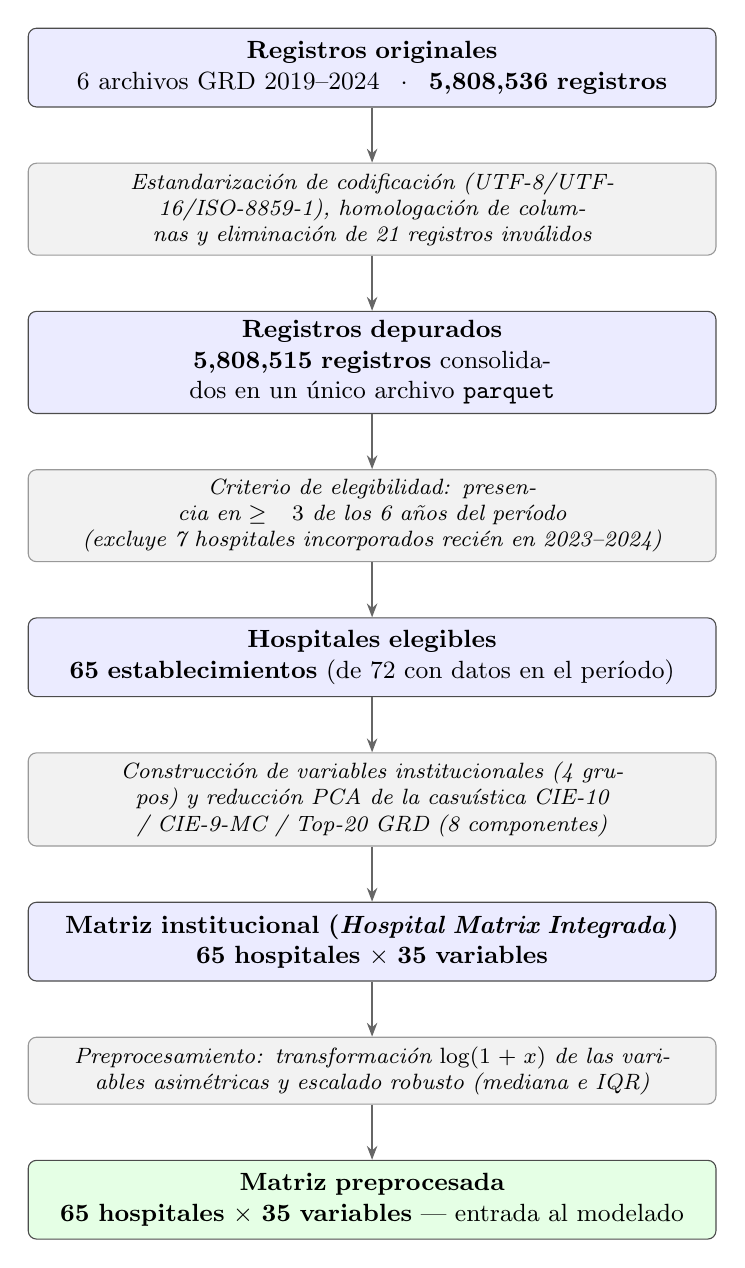
\begin{tikzpicture}[
    node distance = 7mm and 0mm,
    box/.style = {
        rectangle, rounded corners=3pt,
        draw=black!70, fill=white,
        text width=8.5cm, align=center,
        minimum height=1.0cm, font=\small
    },
    filter/.style = {
        rectangle, rounded corners=3pt,
        draw=black!40, fill=black!5,
        text width=8.5cm, align=center,
        minimum height=0.8cm, font=\footnotesize\itshape
    },
    arrow/.style = {-{Stealth[length=5pt]}, thick, black!60}
]

% Nodo 1
\node[box, fill=blue!8] (raw)
    {\textbf{Registros originales}\\
     6 archivos GRD 2019--2024 $\;\cdot\;$ \textbf{5{,}808{,}536 registros}};

% Filtro 1
\node[filter, below=of raw] (f1)
    {Estandarización de codificación (UTF-8/UTF-16/ISO-8859-1),
     homologación de columnas y eliminación de 21 registros inválidos};

% Nodo 2
\node[box, below=of f1, fill=blue!8] (clean)
    {\textbf{Registros depurados}\\
     \textbf{5{,}808{,}515 registros} consolidados en un único archivo \texttt{parquet}};

% Filtro 2
\node[filter, below=of clean] (f2)
    {Criterio de elegibilidad: presencia en $\geq 3$ de los 6 años del período\\
     (excluye 7 hospitales incorporados recién en 2023--2024)};

% Nodo 3
\node[box, below=of f2, fill=blue!8] (hosp)
    {\textbf{Hospitales elegibles}\\
     \textbf{65 establecimientos} (de 72 con datos en el período)};

% Filtro 3
\node[filter, below=of hosp] (f3)
    {Construcción de variables institucionales (4 grupos) y
     reducción PCA de la casuística CIE-10 / CIE-9-MC / Top-20 GRD
     (8 componentes)};

% Nodo 4
\node[box, below=of f3, fill=blue!8] (matrix)
    {\textbf{Matriz institucional (\textit{Hospital Matrix Integrada})}\\
     \textbf{65 hospitales $\times$ 35 variables}};

% Filtro 4
\node[filter, below=of matrix] (f4)
    {Preprocesamiento: transformación $\log(1+x)$ de las variables asimétricas
     y escalado robusto (mediana e IQR)};

% Nodo 5
\node[box, below=of f4, fill=green!10] (scaled)
    {\textbf{Matriz preprocesada}\\
     \textbf{65 hospitales $\times$ 35 variables} — entrada al modelado};

% Flechas
\draw[arrow] (raw)   -- (f1);
\draw[arrow] (f1)    -- (clean);
\draw[arrow] (clean) -- (f2);
\draw[arrow] (f2)    -- (hosp);
\draw[arrow] (hosp)  -- (f3);
\draw[arrow] (f3)    -- (matrix);
\draw[arrow] (matrix) -- (f4);
\draw[arrow] (f4)    -- (scaled);

\end{tikzpicture}
\caption{Flujo de datos desde los registros originales hasta la matriz institucional preprocesada.}
\label{fig:pipeline-datos}
\end{figure}

\subsection{Limitaciones de la fuente}
\label{sec:limitaciones-fuente}

Por tratarse de registros administrativos concebidos con fines de financiamiento
y no de investigación, la base GRD presenta tres limitaciones que deben
considerarse al interpretar los resultados del perfilamiento.

La primera tiene que ver con la exhaustividad diagnóstica. Los hospitales con
mayor dotación de codificadores o con sistemas de apoyo a la codificación tienden
a registrar más diagnósticos secundarios por egreso que aquellos con menor
capacidad técnica, lo que puede inflar artificialmente indicadores como el
promedio de comorbilidades en ciertos establecimientos. Aunque al agregar los
registros a nivel institucional este efecto se distribuye entre todos los egresos
del hospital y pierde parte de su influencia, no desaparece por completo. En
consecuencia, una diferencia entre hospitales en las variables de comorbilidad no
admite una lectura directa como diferencia en la carga clínica de los pacientes
atendidos, porque puede originarse en la práctica de registro de cada centro.

Esta limitación merece una precisión cuantitativa, porque la decisión de leer
la totalidad de los campos de codificación (Sección~\ref{sec:variables}) la
vuelve más visible en lugar de atenuarla. Los 65 hospitales elegibles utilizan
campos más allá del quinto diagnóstico, con una profundidad que va de $0{,}73$ a
$3{,}80$ diagnósticos adicionales por egreso, de modo que la variación en
exhaustividad no afecta a un subconjunto marginal sino a toda la red. Al
descomponer esa variación, el Servicio de Salud al que pertenece el
establecimiento explica un $51\,\%$ de la varianza en profundidad de
codificación, proporción que sugiere un componente institucional o
administrativo y no puramente clínico. Dos elementos acotan esa lectura. Por
una parte, la dispersión dentro de un mismo Servicio de Salud sigue siendo
amplia --en Araucanía Sur la profundidad va de $1{,}28$ a $3{,}80$--, por lo que
el fenómeno no se reduce a un patrón regional homogéneo. Por otra, el aumento
del promedio de comorbilidades al incorporar los campos completos correlaciona
positivamente con la severidad media ($r = 0{,}64$) y con la mortalidad media
($r = 0{,}58$) de cada establecimiento, es decir, se concentra donde la carga
clínica registrada es mayor, lo que es coherente con un componente clínico
genuino. Conviene subrayar que truncar los campos no controlaba este sesgo sino
que lo encubría: bajo un techo de cinco diagnósticos, un hospital que codifica
veinte y otro que codifica cinco resultaban indistinguibles. La cobertura
completa hace la heterogeneidad de registro observable y, por lo mismo,
obligatoria de declarar al interpretar cualquier comparación de comorbilidad
entre establecimientos.

La segunda limitación se relaciona con la estabilidad longitudinal del sistema
GRD y de la producción hospitalaria a lo largo del período. Esta limitación opera
en tres dimensiones.

La primera es la pandemia de COVID-19. Los años 2020 y 2021 presentan caídas
bruscas en el volumen de registros, con 781{,}912 y 816{,}909 egresos
respectivamente, frente a 1{,}151{,}475 en 2019, lo que refleja la contracción de
la actividad electiva durante la crisis sanitaria. Esta disminución no fue uniforme entre
hospitales: los centros de mayor complejidad reconvirtieron actividad hacia la
atención de pacientes críticos, alterando temporalmente sus perfiles de
casuística, índices de severidad, estancias medias y tasas de mortalidad
registrada. Al calcular promedios institucionales sobre los seis años, los
valores de 2020--2021 quedan incluidos con el mismo peso que los años de
actividad normal, lo que puede atenuar diferencias funcionales reales entre
establecimientos. Este efecto no puede eliminarse del pipeline de análisis, y
constituye una razón adicional para interpretar los perfiles como una
caracterización del período en su conjunto y no como representación de la
actividad habitual pre o post pandemia.

La segunda dimensión es la transición del manual que rige la captura y el
procesamiento de los egresos. Los años 2019 y 2020 operaron bajo la versión 4.0
del Manual de Orientación para la Captura y Procesamiento de los Egresos
Hospitalarios, mientras que los años 2022 a 2024 lo hicieron bajo la versión 5.0,
aprobada mediante Resolución Exenta N°~934 del 14 de diciembre de 2021 e
instruida a partir de 2022, correspondiendo el año 2021 a un período de
transición. El alcance real de esta discontinuidad se acotó inspeccionando los
propios archivos. Los seis años reportan el mismo agrupador (IR-GRD 29301) y,
más importante, la relación entre código GRD y peso relativo es constante en
todo el período: entre los 1.064 códigos GRD distintos presentes en la base
depurada, ninguno registra más de un valor de peso relativo ni más de un valor
de índice de severidad a lo largo de los seis años. Es decir, los archivos
públicos emplean una única tabla de pesos e índices, y la transición de versión
no introdujo un reescalamiento de estos atributos. Lo que no puede verificarse
desde los archivos es la asignación misma de los episodios a grupos: un mismo
cuadro clínico podría quedar clasificado en códigos distintos según la versión
vigente, y el conjunto de códigos GRD observados varía moderadamente entre años
(de 1.053 en 2019 a 989 en 2024). Ese margen de incertidumbre, y no una
diferencia de pesos, es el ruido que la transición introduce en los indicadores
de complejidad que cruzan el cambio.

La tercera dimensión es normativa: a partir del 30 de enero de 2023, la Ley de
Presupuestos N°~21.516 exigió registrar bajo estándares GRD el 100\,\% de la
actividad de atención abierta, incluyendo la hospitalización diurna, lo que puede
alterar la composición de los registros de 2023 y 2024 respecto a años anteriores.

Estas tres dimensiones son inherentes a las fuentes públicas disponibles. Su
efecto se mitiga parcialmente al trabajar con promedios institucionales sobre el
período completo, pero no se elimina. Por ello, los resultados del perfilamiento
deben entenderse como una caracterización del período 2019--2024 en su conjunto y
no como una serie temporal de perfiles anuales, con un margen de error en los
indicadores de complejidad mayor que el de las variables de volumen y estancia.

La tercera limitación es de alcance, dado que la base no contiene información sobre
dotación de personal, infraestructura física ni desenlaces clínicos post-alta.
En consecuencia, el perfilamiento describe lo que los hospitales registran durante
la hospitalización y no lo que producen en términos de salud de la población
atendida. Esta restricción proviene del diseño original de la base, que no fue concebida
para capturar resultados clínicos, y no puede resolverse mediante ningún proceso
de limpieza o transformación de los datos, dado que la información simplemente no
está registrada. Sin embargo, esta limitación es coherente con el objetivo del
estudio, que busca caracterizar el perfil funcional de los establecimientos a
partir de su actividad clínica registrada y no evaluar su desempeño en resultados.


\clearpage
\begin{table}[tp]
\centering
\caption{Principales variables del registro GRD y sus tipos de dato.}
\label{tab:variables-grd}
\begin{tabular}{p{4.2cm} p{7.0cm} p{1.8cm}}
\toprule
\textbf{Variable} & \textbf{Descripción} & \textbf{Tipo} \\
\midrule
\multicolumn{3}{l}{\textit{Identificación del establecimiento y paciente}} \\
\addlinespace
\texttt{COD\_HOSPITAL}        & Código del establecimiento tratante           & Código \\
\texttt{CIP\_ENCRIPTADO}      & Identificador encriptado del paciente (hasta 2023) & Código \\
\texttt{ID\_BENEFICIARIO}     & Identificador del beneficiario (desde 2024)   & Código \\
\addlinespace
\multicolumn{3}{l}{\textit{Datos del paciente}} \\
\addlinespace
\texttt{SEXO}                 & Sexo declarado del paciente                   & Texto \\
\texttt{FECHA\_NACIMIENTO}    & Fecha de nacimiento                           & Fecha \\
\texttt{PREVISION}            & Sistema previsional de salud                  & Texto \\
\addlinespace
\multicolumn{3}{l}{\textit{Información hospitalaria}} \\
\addlinespace
\texttt{SERVICIO\_SALUD}      & Servicio de Salud al que pertenece el hospital & Texto \\
\texttt{TIPO\_PROCEDENCIA}    & Origen de la derivación al establecimiento    & Texto \\
\texttt{TIPO\_INGRESO}        & Modalidad de ingreso (urgencia, programado, obstétrico, etc.) & Texto \\
\texttt{TIPO\_ACTIVIDAD}      & Tipo de episodio (hospitalización o CMA)      & Texto \\
\texttt{FECHA\_INGRESO}       & Fecha de ingreso al establecimiento           & Fecha \\
\texttt{FECHA\_ALTA}          & Fecha de egreso del establecimiento           & Fecha \\
\texttt{TIPOALTA}             & Condición de alta (domicilio, traslado, fallecido, etc.) & Texto \\
\texttt{USOSPABELLON}         & Número de usos de pabellón quirúrgico         & Numérico \\
\addlinespace
\multicolumn{3}{l}{\textit{Clasificación GRD}} \\
\addlinespace
\texttt{IR\_29301\_COD\_GRD}  & Código del Grupo Relacionado por Diagnóstico  & Código \\
\texttt{IR\_29301\_PESO}      & Peso relativo del GRD asignado                & Numérico \\
\texttt{IR\_29301\_SEVERIDAD} & Índice de severidad del episodio              & Entero \\
\texttt{IR\_29301\_MORTALIDAD}& Índice de mortalidad del episodio             & Entero \\
\addlinespace
\multicolumn{3}{l}{\textit{Codificación clínica}} \\
\addlinespace
\texttt{DIAGNOSTICO1}--\texttt{35}   & Diagnósticos CIE-10 (principal y comorbilidades) & Código \\
\texttt{PROCEDIMIENTO1}--\texttt{30} & Procedimientos CIE-9-MC                       & Código \\
\bottomrule
\end{tabular}
\end{table}

Los campos identificados como \emph{código} corresponden a etiquetas
categóricas, no a magnitudes: aunque en varios casos se expresan con dígitos,
no admiten operaciones aritméticas y el pipeline los lee como texto para evitar
la pérdida de ceros a la izquierda y de sufijos alfabéticos, presentes por
ejemplo en las secciones de la CIE-9-MC.

\section{Preparación de los datos}
\label{sec:etl}

La etapa de preparación transforma los seis archivos anuales heterogéneos en 
una única base depurada y estandarizada a nivel de registro. El proceso se articula en cinco pasos secuenciales: estandarización y limpieza,
clasificación de la actividad, aplicación de los criterios de elegibilidad,
construcción de variables e ingeniería de características, y
preprocesamiento y normalización.


\subsection{Estandarización y limpieza}
\label{sec:estandarizacion}

Cada archivo anual se lee con su codificación específica según lo indicado en la
Tabla~\ref{tab:heterogeneidad}, y se homologan los nombres de columnas, los
identificadores de establecimiento y los formatos de fecha. A partir de las
fechas de ingreso y alta se derivan dos variables fundamentales para el análisis:
la estancia hospitalaria, expresada en días, y la edad del paciente al momento
del ingreso, calculada desde la fecha de nacimiento. El identificador de paciente, en cambio, no forma parte de las columnas que el
pipeline solicita al leer los archivos: como se detalla en la
Sección~\ref{sec:comprension-negocio}, ninguna variable analítica se construye a
partir de él, de modo que el cambio de nombre de \texttt{CIP\_ENCRIPTADO} a
\texttt{ID\_BENEFICIARIO} en 2024 no exige homologación alguna ni una
equivalencia demostrada entre ambos campos.

En esta fase además se descartan los registros con \texttt{COD\_HOSPITAL} vacío y
aquellos cuya variable \texttt{TIPO\_ACTIVIDAD} no corresponde a ninguna de las
modalidades reconocidas por el estándar GRD. De los 5{,}808{,}536 registros
originales, 21 fueron eliminados por estas razones, todos ellos del año 2019 y
todos por presentar valores no estándar en \texttt{TIPO\_ACTIVIDAD}:
específicamente las categorías \texttt{DESCONOCIDO} (18 registros) y
\texttt{NO IDENTIFICADO} (3 registros), que no pueden asignarse a ninguna
modalidad de análisis. El criterio de \texttt{COD\_HOSPITAL} vacío se mantiene
como control de integridad, pero no descartó ningún registro: los seis archivos
identifican el establecimiento tratante en la totalidad de sus filas. Cabe
destacar que tampoco fue eliminado ningún registro por estancia negativa ni por
fechas inválidas, dado que ambas condiciones se trataron mediante truncamiento y
conversión a nulo respectivamente, conservando el registro en la base. El
resultado es una base depurada de 5{,}808{,}515 registros, lo que confirma que
los archivos GRD presentan alta consistencia interna. Los seis archivos anuales depurados se consolidan en
un único archivo en formato \texttt{parquet}, que permite su consulta eficiente
sin necesidad de cargar el conjunto completo en memoria.

\subsection{Clasificación de la actividad}
\label{sec:clasificacion-actividad}

El sistema GRD chileno registra episodios de hospitalización bajo cuatro tipos de
actividad. La hospitalización convencional corresponde a ingresos con estadía
nocturna en cama asignada, ya sea de origen programado o electivo, donde el
paciente permanece al menos una noche en el establecimiento. La hospitalización
en urgencia es un subconjunto que identifica específicamente los episodios
ingresados por la vía de urgencia que derivan en estadía nocturna. La
hospitalización diurna, en cambio, agrupa atenciones que requieren cama y
procedimientos durante el día pero que no implican estadía nocturna, como
quimioterapia, transfusiones o procedimientos de corta duración. La cirugía mayor
ambulatoria (CMA) agrupa procedimientos quirúrgicos o de alto costo que se
resuelven sin estadía nocturna, con alta el mismo día de la
intervención~\citep{TableauGRD}.

La distinción entre hospitalización convencional y CMA es relevante para el
perfilamiento porque ambas modalidades responden a lógicas funcionales distintas.
La CMA se asocia a procedimientos electivos de baja complejidad relativa y
estancia nula o mínima, mientras que la hospitalización convencional concentra los
episodios de mayor duración, severidad y consumo de recursos. Incorporar ambas en
los mismos indicadores de estancia y peso GRD distorsionaría los perfiles, por lo
que los indicadores se calculan por separado según modalidad. La distribución
de los registros por tipo de actividad se presenta en la
Tabla~\ref{tab:actividad}.


\begin{table}[htbp]
\centering
\caption{Distribución de registros por tipo de actividad tras la limpieza.}
\label{tab:actividad}
\begin{tabular}{lrr}
\toprule
\textbf{Tipo de actividad} & \textbf{Registros} & \textbf{\%} \\
\midrule
Hospitalización convencional     & 4{,}800{,}768 & 82{,}6 \\
Cirugía mayor ambulatoria (CMA)  &   889{,}868   & 15{,}3 \\
Hospitalización en urgencia      &    62{,}551   &  1{,}1 \\
Hospitalización diurna           &    55{,}328   &  1{,}0 \\
\midrule
\textbf{Total}                   & \textbf{5{,}808{,}515} & \textbf{100{,}0} \\
\bottomrule
\end{tabular}
\end{table}

\subsection{Criterios de elegibilidad}
\label{sec:elegibilidad}

La base depurada abarca 72 establecimientos con datos GRD en el período. Para
garantizar que los indicadores agregados sean comparables entre hospitales, se
aplica un criterio de inclusión: presencia en al menos tres de los seis años
del período. Este umbral responde a que los indicadores institucionales como
la estancia media, la proporción de CMA o la diversidad diagnóstica son
estimaciones estadísticas que requieren varios años de observación para no
depender de las particularidades de un único año. Un establecimiento con
datos en uno o dos años podría presentar valores atípicos debidos a factores
circunstanciales como cierres temporales, cambios de gestión o
incorporación reciente al sistema de información, que no reflejan su perfil
funcional habitual.

Una primera observación empírica reduce la relevancia práctica de elegir un
punto de corte exacto: la distribución real de años presentes entre los 72
establecimientos de la base depurada es marcadamente bimodal. Como muestra la
Tabla~\ref{tab:distribucion-anios}, 4 hospitales reportan datos en un único
año y 3 en dos años, todos ellos incorporados al sistema de información
recién en 2023 o 2024, mientras que los 65 hospitales restantes reportan
los seis años completos del período. Ningún establecimiento del
universo real tiene exactamente 3, 4 o 5 años de datos. En consecuencia,
cualquier umbral situado en ese rango (3, 4 o 5) produce exactamente el mismo
universo final de 65 hospitales elegibles: la elección del valor específico
``3'' no es, en los hechos, una decisión consecuente sobre qué establecimientos
se incluyen o excluyen, sino que opera sobre un vacío natural de los datos.

\begin{table}[htbp]
\centering
\caption{Distribución de años con datos GRD entre los 72 establecimientos de la base depurada.}
\label{tab:distribucion-anios}
\begin{tabular}{c c l}
\toprule
\textbf{Años presentes} & \textbf{N.º de hospitales} & \textbf{Interpretación} \\
\midrule
1 & 4  & Incorporación reciente (2023--2024) \\
2 & 3  & Incorporación reciente (2023--2024) \\
3--5 & 0  & (vacío en los datos reales) \\
6 & 65 & Cobertura completa del período \\
\bottomrule
\end{tabular}
\end{table}

Para cuantificar el segundo aspecto de la observación, se realizó
una simulación de error por submuestreo sobre los 65 hospitales con cobertura
completa. Tomando el valor de cada indicador calculado con los seis años como
referencia (``verdad''), se recalculó el mismo indicador usando todas las
combinaciones posibles de $k \in \{1, 2, 3, 4, 5\}$ años (o una muestra
aleatoria de 200 combinaciones cuando el total de combinaciones superaba ese
valor) y se midió el error relativo absoluto resultante, con un intervalo de
confianza del 95\,\% obtenido por bootstrap sobre la mediana. La
Tabla~\ref{tab:simulacion-anios} resume el error relativo mediano para las
seis variables tradicionales del pipeline.

\begin{table}[htbp]
\centering
\caption{Error relativo mediano (\%) al estimar cada indicador institucional con $k$ años en lugar de los 6 años completos, con intervalo de confianza 95\,\% (\textit{bootstrap}).}
\label{tab:simulacion-anios}
\begin{tabular}{c c c c c c c}
\toprule
\textbf{$k$ años} & \textbf{Egresos/año} & \textbf{Estancia} & \textbf{Peso GRD} & \textbf{Severidad} & \textbf{Mortalidad} & \textbf{Tasa CMA} \\
\midrule
1 & 9{,}3\,\% & 5{,}8\,\% & 4{,}2\,\% & 4{,}6\,\% & 3{,}8\,\% & 21{,}3\,\% \\
2 & 6{,}0\,\% & 4{,}5\,\% & 4{,}9\,\% & 3{,}8\,\% & 3{,}2\,\% & 10{,}9\,\% \\
\textbf{3} & \textbf{4{,}5\,\%} & \textbf{3{,}3\,\%} & \textbf{3{,}6\,\%} & \textbf{2{,}8\,\%} & \textbf{2{,}4\,\%} & \textbf{8{,}0\,\%} \\
4 & 3{,}0\,\% & 2{,}2\,\% & 2{,}4\,\% & 1{,}9\,\% & 1{,}6\,\% & 5{,}3\,\% \\
5 & 1{,}9\,\% & 1{,}1\,\% & 0{,}8\,\% & 0{,}9\,\% & 0{,}7\,\% & 4{,}2\,\% \\
\bottomrule
\end{tabular}
\end{table}

El error decrece de forma monótona con $k$ para las seis variables, pero el patrón de la reducción marginal es lo que sustenta el
umbral adoptado: el error promedio (sobre las seis variables) cae de
$8{,}2\,\%$ con un año a $4{,}1\,\%$ con tres años (una reducción de
$4{,}1$ puntos porcentuales) mientras que agregar un cuarto y un quinto año
reduce el error en $1{,}4$ y $1{,}2$ puntos porcentuales adicionales,
respectivamente. Es decir, el mayor beneficio marginal de sumar años se
obtiene entre $k=1$ y $k=3$. A partir de tres años, cada año adicional
reduce el error a una tasa aproximadamente constante y sustancialmente menor
que en el tramo inicial. Este patrón de rendimientos decrecientes, y no una
referencia externa, es lo que justifica fijar el umbral en tres años: es el
primer punto en el que la reducción del error empieza a estabilizarse. La
única excepción es la tasa de CMA, cuyo error relativo permanece
comparativamente alto incluso con tres años ($8{,}0\,\%$), lo esperable dado
que es una proporción calculada sobre un subconjunto minoritario de egresos
(los de modalidad CMA) y por tanto más sensible a la variación año a año que
los indicadores calculados sobre la totalidad de los egresos de
hospitalización.

Con esta evidencia, el umbral de tres años se sostiene como un punto de
compromiso cuantificado no arbitrario, aunque tampoco derivado de una regla
de decisión formal única entre la reducción de error que ofrece cada año
adicional de datos y el tamaño del universo de análisis disponible. El
detalle completo de la simulación (código, valores por hospital y por
combinación de años) se encuentra en
los artefactos de análisis reproducibles y la documentación de resultados del repositorio del
proyecto.

La aplicación de este criterio reduce el conjunto a 65 establecimientos, que
constituyen la población de análisis sobre la cual se construye la matriz
institucional descrita en la sección siguiente. El efecto de este criterio sobre
la partición final, y no solo sobre el error de los indicadores, se evalúa
mediante el análisis de sensibilidad definido en la
Sección~\ref{sec:sensibilidad-elegibilidad}.

La Tabla~\ref{tab:descartados} detalla los siete establecimientos excluidos, los
años en que reportaron datos y el total de egresos registrados en el período.
\begin{table}[htbp]
\centering
\caption{Establecimientos excluidos por no cumplir el criterio de presencia temporal.}
\label{tab:descartados}
\begin{tabular}{p{6.2cm} p{3.8cm} p{1.8cm} r}
\toprule
\textbf{Establecimiento} & \textbf{Servicio de Salud} & \textbf{Años con datos} & \textbf{Egresos} \\
\midrule
Instituto Traumatológico Dr. T. Gebauer & Metropolitano Suroriente & 2023, 2024 & 6{,}206 \\
Hospital de Constitución                & Del Maule               & 2024       & 2{,}796 \\
Hospital San Juan de Dios (Cauquenes)   & Del Maule               & 2024       & 4{,}461 \\
Hospital de Lota                        & Concepción              & 2023, 2024 & 7{,}706 \\
Hospital de Tomé                        & Talcahuano              & 2023, 2024 & 6{,}365 \\
Hospital Penco-Lirquén                  & Concepción              & 2024       & 2{,}751 \\
Complejo Asistencial Padre Las Casas    & Araucanía Sur           & 2024       & 6{,}389 \\
\bottomrule
\end{tabular}
\end{table}

\subsection{Construcción de variables e ingeniería de características}
\label{sec:variables}

A partir de los registros depurados se construye un conjunto de aproximadamente
35 variables agregadas a nivel institucional, organizadas en cuatro grupos
conceptuales. Una decisión metodológica central es la exclusión de recursos de infraestructura y equipamiento tales como la dotación de camas o ambulancias, dado que el objetivo es un perfilamiento funcional y no
estructural, todas las variables se derivan exclusivamente de la actividad clínica
registrada, de modo que los grupos resultantes reflejen lo que los hospitales
hacen y no la capacidad física que poseen.

Una segunda decisión de diseño es utilizar la totalidad de los campos de
codificación clínica disponibles. Aunque el registro GRD admite hasta 35
diagnósticos CIE-10 y hasta 30 procedimientos CIE-9-MC por egreso
(Tabla~\ref{tab:variables-grd}), el pipeline detecta dinámicamente y procesa
\texttt{DIAGNOSTICO1}--\texttt{DIAGNOSTICO35} y
\texttt{PROCEDIMIENTO1}--\texttt{PROCEDIMIENTO30}. Para controlar el costo de
memoria de procesar 65 campos clínicos sobre 5{,}8 millones de registros, los
conteos se acumulan columna a columna en vez de materializar una tabla extensa
de todos los códigos. Así, el promedio de comorbilidades corresponde al número
medio de diagnósticos secundarios registrados entre
\texttt{DIAGNOSTICO2} y \texttt{DIAGNOSTICO35}, con rango teórico $[0,34]$,
y los vectores ponderados de capítulos CIE-10 y de secciones CIE-9-MC reflejan
la codificación completa del episodio.

Esta cobertura evita subrepresentar los egresos con mayor profundidad de
registro, pero no elimina la heterogeneidad de codificación entre
establecimientos. Por ello, las diferencias en comorbilidades deben interpretarse
como diferencias en carga clínica \emph{registrada}, potencialmente afectadas por
la exhaustividad de codificación de cada centro, y no como una medida clínica
pura. El análisis conserva los indicadores porque incorporan información
relevante para el perfilamiento relativo, y declara esta limitación al
interpretar los resultados.

\clearpage
La Tabla~\ref{tab:variables} sintetiza las variables construidas por grupo.

{\small
\setstretch{1.0}
\setlength{\LTleft}{0pt}
\setlength{\LTright}{\fill}
\begin{longtable}{>{\raggedright\arraybackslash}p{3.2cm} >{\raggedright\arraybackslash}p{8.5cm}}
\caption{Variables construidas a nivel institucional, agrupadas por dimensión.}
\label{tab:variables} \\
\toprule
\textbf{Grupo} & \textbf{Variables} \\
\midrule
\endfirsthead
\multicolumn{2}{l}{\small\textit{Tabla~\thetable\ (continuación)}} \\
\toprule
\textbf{Grupo} & \textbf{Variables} \\
\midrule
\endhead
\bottomrule
\endfoot
\raggedright Tradicionales de gestión &
Egresos por año, estancia media, estancia mediana, peso medio GRD, índice de
severidad medio, índice de mortalidad medio. \\
\addlinespace
\raggedright Diversidad diagnóstica &
Entropía de Shannon normalizada sobre la distribución de GRD, comorbilidades
promedio por egreso (diagnósticos secundarios 2 a 35, rango teórico $[0,34]$). \\
\addlinespace
\raggedright Cirugía mayor ambulatoria &
Tasa de CMA, peso medio de los GRD de CMA. \\
\addlinespace
\raggedright Perfil funcional agregado &
Distribución demográfica (\% pediátrico, \% geriátrico, \% femenino fértil), mezcla
por tipo de ingreso (\% urgencia, \% programado, \% referencia), tipo de alta (\%
domicilio, \% traslado, \% fallecido), uso de pabellón, actividad obstétrica (tasa
de partos, \% obstétrica, tasa de prematurez), dispersión de la estancia
(coeficiente de variación). \\
\bottomrule
\end{longtable}
}

\textbf{Variables tradicionales de gestión:} Este grupo captura los indicadores de producción y complejidad habituales en la
gestión hospitalaria. El peso medio GRD es especialmente relevante porque resume
en un único valor la intensidad de recursos esperada para la casuística promedio
del establecimiento, mientras que los índices de severidad y mortalidad reflejan
la gravedad clínica de la población atendida.

\textbf{Variables de diversidad diagnóstica:} Para cuantificar la amplitud del espectro clínico de cada hospital se emplea la
entropía de Shannon normalizada sobre la distribución de GRD. Dada la
distribución de frecuencias relativas $p_i$ de los $G$ grupos GRD distintos
presentes en un hospital, el indicador se define como:

\begin{equation}
H_{\text{norm}} = \frac{-\sum_{i=1}^{G} p_i \, \log_2(p_i)}{\log_2 G}
\label{eq:shannon}
\end{equation}

La división por $\log_2 G$, que es el valor máximo que puede alcanzar la
entropía cuando la distribución es uniforme, acota el indicador al intervalo
$[0, 1]$ y lo hace comparable entre hospitales con distinto número de GRD
distintos; por convención se asigna el valor 0 cuando $G \leq 1$ y se excluyen
los términos con $p_i = 0$. Un hospital con entropía normalizada alta atiende una
gran variedad de condiciones con frecuencias relativamente uniformes (perfil
generalista), mientras que uno con entropía baja concentra su actividad en pocos
grupos (perfil especializado). Esta métrica complementa los indicadores de
complejidad al capturar la diversidad de la producción.

\textbf{Variables de cirugía mayor ambulatoria:} La tasa de CMA y el peso medio de sus GRD caracterizan la orientación ambulatoria del establecimiento, una combinación que resulta especialmente informativa, ya que una tasa alta con peso bajo señala un perfil orientado a procedimientos electivos simples, mientras que una tasa alta con peso elevado indica un programa de CMA de mayor complejidad técnica en el establecimiento. Cabe precisar que, de estas dos variables, solo la tasa de CMA integra la matriz sobre la que opera el agrupamiento: el peso medio de CMA no está definido para los establecimientos sin actividad de esta modalidad, por lo que se conserva con fines exclusivamente descriptivos y se excluye del modelado, como se detalla en la Sección~\ref{sec:matriz-final}.

\textbf{Variables de perfil funcional agregado:}
Este grupo, el más numeroso, describe la composición de la actividad clínica
mediante proporciones calculadas exclusivamente sobre los egresos de
hospitalización (excluyendo CMA). La separación no responde a ausencia de información: los campos demográficos,
de ingreso, alta, procedencia y pabellón también están disponibles en los
episodios CMA. Responde a que la CMA es una modalidad ambulatoria: en los datos, el $93{,}3\,\%$ de sus episodios registra estancia igual a cero. Mezclarla con hospitalización alteraría el significado y los denominadores de indicadores definidos para hospitalización. Por ejemplo, un
hospital con mayor proporción de CMA reduciría mecánicamente sus tasas de
estancia prolongada o de ingreso obstétrico, aun sin modificar su perfil de
hospitalización. La orientación ambulatoria no se omite:
se incorpora separadamente mediante la tasa de CMA, mientras que el peso medio
de los GRD de CMA se conserva como variable descriptiva. Cada variable de este
bloque se define operacionalmente como la fracción de egresos hospitalarios que
cumple una condición, lo que las hace comparables entre hospitales de distinto
volumen. La Tabla~\ref{tab:definiciones} detalla sus definiciones operacionales.

\begin{table}[htbp]
\centering
\caption{Definiciones operacionales de las variables de perfil funcional
agregado.}
\label{tab:definiciones}
\begin{tabular}{p{5.2cm} p{7.0cm}}
\toprule
\textbf{Variable} & \textbf{Definición operacional} \\
\midrule
\% pediátrico & Proporción de egresos con edad al ingreso menor a 15 años. \\
\% geriátrico & Proporción de egresos con edad al ingreso mayor o igual a 65
años. \\
\% femenino fértil & Proporción de egresos de mujeres entre 15 y 49 años. \\
Edad mediana & Mediana de la edad al ingreso de los egresos. \\
\% urgencia / programada / obstétrica & Proporción de egresos según tipo de
ingreso. \\
\% alta domicilio / fallecido / traslado & Proporción de egresos según tipo de
alta. \\
\% origen emergencia / referencia & Proporción según procedencia del paciente
(servicio de urgencia propio vs.\ derivación de otro establecimiento). \\
\% uso de pabellón & Proporción de egresos con al menos un uso de pabellón
quirúrgico. \\
Tasa de partos & Proporción de egresos con condición de alta neonatal registrada.
\\
Tasa de prematurez & Proporción de partos con peso del recién nacido inferior a
2.500 g. \\
\% estancia larga & Proporción de egresos con estancia superior a 30 días. \\
CV de estancia & Coeficiente de variación de la duración de estancia. \\
\bottomrule
\end{tabular}
\end{table}

Estas variables permiten distinguir perfiles funcionales específicos. Una alta
tasa de partos y proporción obstétrica caracteriza a establecimientos con
maternidad activa, mientras que una alta proporción pediátrica identifica
hospitales de niños. De forma similar, una elevada proporción de origen por
referencia señala centros que operan como referentes de su red territorial. A
estas dimensiones se suman el coeficiente de variación de la estancia y la
proporción de estancias largas, que en conjunto capturan la heterogeneidad
interna del proceso de hospitalización y complementan los perfiles anteriores
con información sobre la variabilidad de la gestión clínica dentro de cada
establecimiento.


\subsubsection{Reducción dimensional de la casuística clínica}
\label{sec:pca}

La casuística clínica de cada hospital se resume mediante tres vectores de
proporciones construidos sobre sus egresos. El primero corresponde a la
distribución por los 22 capítulos de la CIE-10. El segundo recoge la
distribución por las 18 secciones de procedimientos definidas en la tabla
maestra CIE-9-MC empleada, es decir, las 17 secciones numeradas de 00 a 16 y la
sección 03A. El tercero describe la concentración del establecimiento en los
20 GRD más frecuentes a nivel nacional. Cada vector incluye una categoría
residual. En los dos primeros casos reúne los códigos que no admiten mapeo a un
capítulo o una sección de la tabla maestra; en el tercero agrupa los GRD que
quedan fuera del Top-20 nacional. Estas categorías permiten que cada vector
forme una distribución completa cuya suma es igual a 1.

Al concatenar los tres vectores se obtiene una matriz de $65 \times 63$
columnas: 23 de capítulos CIE-10, 19 de secciones CIE-9-MC y 21 de GRD, con la
categoría residual incluida en cada caso. Usar directamente esta matriz para
solo 65 hospitales introduce un problema de alta dimensionalidad relativa. En
ese escenario, las distancias entre observaciones pierden capacidad
discriminatoria, el agrupamiento se vuelve inestable y la interpretación se
dificulta, como se argumentó en la Sección~\ref{sec:reduccion}. Por ello, antes
de integrar la casuística con el resto de las variables se aplica PCA para
reducir las 63 columnas a un conjunto compacto de componentes principales.

Estos tres vectores son, en sentido estricto, datos composicionales, pues cada
fila es una distribución de proporciones que suma 1. Aplicar PCA y, más
adelante, distancia euclidiana directamente sobre estas proporciones puede
introducir el problema de la \emph{clausura composicional} (\textit{closure
problem}). Como las partes deben sumar una constante, el incremento de una
proporción obliga necesariamente a la disminución de otras. Esto puede generar
correlaciones y distancias artificiales que no reflejan diferencias reales en la
actividad clínica. La Sección~\ref{sec:sensibilidad-composicional} define el
análisis que evalúa empíricamente la magnitud de este efecto sobre los
resultados del trabajo.

\subsubsection{Análisis de componentes principales}
\label{sec:pca-detalle}

Sobre la matriz concatenada de casuística, previa estandarización de las
proporciones, se aplica PCA. Dado que el vector de capítulos CIE-10 admite dos
construcciones, se evaluaron ambas variantes de forma independiente. La variante
\emph{principal} considera únicamente el diagnóstico principal
(\texttt{DIAGNOSTICO1}) de cada egreso, de modo que cada egreso aporta una
unidad al capítulo de su causa de hospitalización. La variante \emph{ponderada}
incorpora además los diagnósticos secundarios registrados, asignando peso
$1{,}0$ al diagnóstico principal y $0{,}5$ a cada secundario, con el propósito
de reflejar las comorbilidades del episodio sin que estas lleguen a dominar
sobre el motivo principal de ingreso. La ponderación es, por tanto, por posición
del diagnóstico dentro del episodio y no por el peso relativo del GRD asignado.
La comparación entre ambas variantes se resolvió mediante un criterio interno al
propio PCA:
para cada variante se ejecutó el PCA con el número de componentes fijado en
$K=8$ (justificado más adelante en esta sección) y se comparó la varianza
acumulada explicada, sin recurrir a ninguna métrica de clustering posterior.
La variante ponderada explica el 72{,}3\,\% de la varianza acumulada frente al
71{,}8\,\% de la variante basada solo en el diagnóstico principal, por lo que fue seleccionada
para el pipeline definitivo. Este criterio de selección --varianza explicada
por el propio PCA-- es deliberadamente independiente del clustering que se
describe en las secciones siguientes, para evitar que la elección de una
decisión de preprocesamiento quede determinada por la misma métrica con la
que luego se evalúa la solución final. Esta misma comparación se repite bajo una
representación composicional alternativa (CLR) como parte del análisis de
sensibilidad definido en la Sección~\ref{sec:sensibilidad-composicional}.

El número de componentes a retener se fija en $K=8$, decisión que se
verificó empíricamente mediante un barrido de $K \in \{8, 9, 10, 11\}$
evaluando el efecto de cada valor sobre las métricas de validación interna
del clustering final (Tabla~\ref{tab:barrido-k-pca}). Con la variante
ponderada, las 8 componentes explican el 72{,}3\,\% de la varianza acumulada
de las 63 columnas de casuística. Incorporar componentes adicionales
incrementa la varianza retenida, pero no mejora la calidad de la partición
resultante. Por el contrario, al aumentar $K$ de 8 a 11 --el número mínimo
que acumularía el 80\,\% de la varianza-- el coeficiente de Silhouette
desciende de $0{,}401$ a $0{,}380$, el índice de Calinski-Harabasz cae de
$22{,}4$ a $19{,}7$ y el índice de Davies-Bouldin empeora de $0{,}990$ a
$1{,}076$. El valor $K=9$ obtiene el mejor Silhouette del barrido
($0{,}422$), pero fragmenta los grupos especializados de forma menos
interpretable que $K=8$: reintroduce un grupo de apenas dos establecimientos
(tamaños $3$, $54$, $2$, $6$ frente a $3$, $54$, $5$, $3$), precisamente la
situación en que las pruebas de significancia basadas en aproximaciones
asintóticas pierden validez (Sección~\ref{sec:nivel2-metodo}). Se retienen,
por tanto, las 8 componentes por ser el valor que ofrece el mejor balance
entre las tres métricas de validación interna y la interpretabilidad de los
grupos resultantes, y no un porcentaje de varianza explicada fijado de
antemano: agregar componentes de casuística más allá de este punto introduce
ruido de alta dimensionalidad relativa (Sección~\ref{sec:pca}) que degrada la
cohesión y separación del clustering en mayor medida que lo que aporta en
varianza retenida.

\begin{table}[htbp]
\centering
\caption{Efecto del número de componentes PCA de casuística ($K$) sobre las métricas de validación interna del clustering Ward $K=4$.}
\label{tab:barrido-k-pca}
\begin{tabular}{c c c c c l}
\toprule
\textbf{$K$ (componentes)} & \textbf{Varianza acum.} & \textbf{Silhouette} & \textbf{CH} & \textbf{DB} & \textbf{Tamaños} \\
\midrule
\bfseries 8 & \bfseries 72{,}3\,\% & 0{,}401 & \bfseries 22{,}4 & \bfseries 0{,}990 & 3, 54, 5, 3 \\
9 & 75{,}2\,\% & \bfseries 0{,}422 & 21{,}9 & 0{,}991 & 3, 54, 2, 6 \\
10 & 77{,}7\,\% & 0{,}384 & 20{,}4 & 1{,}045 & 3, 54, 5, 3 \\
11 & 80{,}0\,\% & 0{,}380 & 19{,}7 & 1{,}076 & 3, 54, 5, 3 \\
\bottomrule
\end{tabular}
\par\smallskip
\begin{minipage}{\textwidth}
\footnotesize\raggedright
\textit{Nota.} CH corresponde al índice de Calinski--Harabasz (un valor mayor indica mejor separación entre grupos); DB corresponde al índice de Davies--Bouldin (un valor menor indica grupos más compactos y separados).
\end{minipage}
\end{table}

Cada componente admite una lectura interpretable a partir de sus cargas. La
Tabla~\ref{tab:cargas-pca} reporta, para cada una de las 8 componentes, las
tres variables originales con mayor magnitud de carga y su signo, lo que
permite sostener empíricamente su interpretación clínica en lugar de
describirla solo en términos generales.

{\footnotesize
\setstretch{1.0}
\setlength{\LTleft}{0pt}
\setlength{\LTright}{\fill}
\begin{longtable}{@{}>{\raggedright\arraybackslash}p{1.4cm}@{\hspace{0.25cm}}>{\raggedright\arraybackslash}p{3.45cm}@{\hspace{0.25cm}}>{\raggedright\arraybackslash}p{3.45cm}@{\hspace{0.25cm}}>{\raggedright\arraybackslash}p{3.45cm}@{}}
\caption{Tres cargas de mayor magnitud por componente PCA de casuística. El signo indica la dirección de la carga.}
\label{tab:cargas-pca} \\
\toprule
\textbf{Componente} & \textbf{Carga 1} & \textbf{Carga 2} & \textbf{Carga 3} \\
\midrule
\endfirsthead
\multicolumn{4}{l}{\footnotesize\textit{Tabla~\thetable\ (continuación)}} \\
\toprule
\textbf{Componente} & \textbf{Carga 1} & \textbf{Carga 2} & \textbf{Carga 3} \\
\midrule
\endhead
\bottomrule
\endfoot
\texttt{dim\_01} & $-$ Embarazo, parto y puerperio ($-0{,}24$) & $+$ Otros GRD fuera del Top-20 ($0{,}23$) & $-$ Procedimientos obstétricos ($-0{,}22$) \\
\addlinespace[3pt]
\texttt{dim\_02} & $-$ Enfermedades de la piel y tejido subcutáneo ($-0{,}27$) & $+$ Operaciones sobre el sistema nervioso ($0{,}24$) & $+$ Operaciones sobre el sistema endocrino ($0{,}23$) \\
\addlinespace[3pt]
\texttt{dim\_03} & $-$ Enfermedades del aparato circulatorio ($-0{,}32$) & $+$ Operaciones sobre el oído ($0{,}27$) & $+$ Malformaciones congénitas y anomalías cromosómicas ($0{,}25$) \\
\addlinespace[3pt]
\texttt{dim\_04} & $-$ PH procedimientos sobre extremidad superior ($-0{,}34$) & $-$ PH procedimientos sobre rodilla y extremidad inferior ($-0{,}31$) & $-$ Operaciones sobre el aparato musculoesquelético ($-0{,}31$) \\
\addlinespace[3pt]
\texttt{dim\_05} & $+$ Operaciones sobre el aparato respiratorio ($0{,}30$) & $-$ Enfermedades del ojo y sus anexos ($-0{,}27$) & $-$ Trastornos mentales y de comportamiento ($-0{,}26$) \\
\addlinespace[3pt]
\texttt{dim\_06} & $+$ Operaciones sobre el aparato digestivo ($0{,}37$) & $+$ Otros procedimientos diagnósticos y terapéuticos ($0{,}33$) & $+$ Operaciones sobre el sistema hemático y linfático ($0{,}32$) \\
\addlinespace[3pt]
\texttt{dim\_07} & $+$ PH colecistectomía laparoscópica ($0{,}36$) & $-$ MH trastornos del anteparto con complicaciones ($-0{,}33$) & $+$ PH cesárea ($0{,}26$) \\
\addlinespace[3pt]
\texttt{dim\_08} & $-$ Operaciones sobre el sistema endocrino ($-0{,}28$) & $+$ MH trastornos del anteparto con complicaciones ($0{,}26$) & $-$ Otros procedimientos diagnósticos y terapéuticos ($-0{,}22$) \\
\bottomrule
\end{longtable}
}

Estas componentes, denotadas \texttt{dim\_01} a \texttt{dim\_08}, reemplazan
las 63 columnas originales de casuística, condensando el perfil
clínico-quirúrgico de cada hospital en un espacio compacto interpretable. Las
cargas completas de las 8 componentes sobre las 63 variables originales se
reportan en el archivo \texttt{reports/tables/reduccion\_dimensional.csv} del
repositorio del proyecto.

\subsubsection{Matriz final de variables}
\label{sec:matriz-final}
La integración de los cuatro grupos de
variables institucionales directas junto con las 8 componentes principales de
casuística conforma la matriz de trabajo definitiva, denominada
\textit{Hospital Matrix Integrada}:

\begin{equation}
  \underbrace{27}_{\text{variables directas}} + \underbrace{8}_{\text{componentes PCA}} = \mathbf{35 \text{ columnas}}
\end{equation}

Las 27 variables directas se distribuyen en 6 tradicionales de gestión, 2 de
diversidad diagnóstica, 1 de cirugía mayor ambulatoria (la tasa de CMA) y 18 de
perfil funcional agregado. La segunda variable de CMA construida en la
Sección~\ref{sec:variables}, el peso medio de los GRD de esta modalidad, queda
fuera de la matriz de modelado porque no está definida para los establecimientos
que no registran actividad ambulatoria en el período: mantenerla habría exigido
imputar un valor arbitrario en esos casos o eliminar hospitales del universo de
análisis. Se conserva, por tanto, únicamente como variable descriptiva en la
caracterización de los perfiles.

Esta matriz tiene dimensiones de $65 \times 35$, donde cada fila representa un
hospital y cada columna una característica derivada exclusivamente de su actividad
clínica. Las 63 columnas originales de casuística no forman parte de la matriz
final, ya que fueron sustituidas íntegramente por las 8 componentes PCA. Sobre esta
matriz opera todo el pipeline de agrupamiento, validación e interpretación
descrito en las secciones siguientes.

\subsection{Preprocesamiento y normalización}
\label{sec:preprocesamiento}

Antes del agrupamiento, las variables se someten a transformaciones
secuenciales orientadas a reducir la influencia de distribuciones con cola
pronunciada y a hacer comparables las escalas de los indicadores en el cálculo
de distancias euclidianas.

\textbf{Transformación logarítmica:} Se aplicó la transformación $\log(1+x)$
a las variables \textit{egresos por año} y \textit{pabellones promedio}, ambas
con asimetría positiva. El volumen anual de egresos varía entre 2.663 y 39.066,
con una asimetría de $0{,}94$, lo que refleja la presencia de algunos
establecimientos de gran tamaño relativo. El promedio de usos de pabellón
presenta la mayor asimetría positiva del conjunto ($2{,}01$), concentrando a la
mayoría de los hospitales en valores bajos y a unos pocos en valores elevados.
Para ambas variables se utilizó:

\begin{equation}
x' = \log(1 + x)
\label{eq:log1p}
\end{equation}

La transformación reduce la influencia de los valores altos sobre las distancias
entre hospitales y evita la indeterminación de $\log(x)$ cuando $x = 0$. La edad
mediana no se transformó logarítmicamente: presenta asimetría negativa
($-1{,}38$), y $\log(1+x)$ está orientada a comprimir colas derechas, por lo que
su aplicación habría acentuado ese patrón. Las variables restantes no se
transformaron logarítmicamente, pues no presentaban colas derechas de magnitud
comparable; sus diferencias de escala se abordan mediante el escalado robusto.

\textbf{Escalado robusto:} Posteriormente, todas las variables de la matriz,
incluidas las transformadas, se estandarizaron mediante un escalador robusto que
las centra en la mediana y las escala por el rango intercuartílico (IQR):

\begin{equation}
z = \frac{x' - \operatorname{mediana}(x')}{\operatorname{IQR}(x')}
\label{eq:robust}
\end{equation}

En las variables que no requirieron transformación logarítmica, $x'$ corresponde
a su valor original. La elección de estos estadísticos frente a los clásicos
basados en media y desviación estándar responde a la presencia de valores
extremos legítimos en la red. El Hospital Sótero del Río, por ejemplo, registra
el mayor volumen de egresos del sistema con 39.066 egresos anuales, cifra que no
constituye un error de registro sino una realidad operativa. Un escalador clásico
sería arrastrado por este extremo, comprimiendo artificialmente la escala del
resto de los hospitales. El escalador robusto atenúa este efecto al basar la
estandarización en la mediana y el IQR, que son resistentes a valores extremos,
y permite conservar estos establecimientos en el análisis.

Como verificación de sensibilidad, se comparó la partición Ward con $K=4$
obtenida con y sin transformación logarítmica de la edad mediana. Ambas
configuraciones produjeron la misma partición de los 65 hospitales
(ARI $= 1{,}00$), por lo que la corrección mejora la coherencia del
preprocesamiento sin alterar los perfiles funcionales reportados.

\subsubsection{Diagnóstico y sensibilidad de bloques de variables}
\label{sec:bloques-variables}

Dado que la distancia euclidiana acumula la contribución de cada variable, se
cuantificó la fracción de la suma de distancias cuadradas entre todos los pares
de hospitales atribuible a cuatro macro-bloques de la matriz ya preprocesada:
gestión, diversidad y CMA (9 variables); perfil operativo no demográfico (11);
demanda demográfica-obstétrica (7); y componentes PCA de casuística (8). El
bloque demográfico-obstétrico comprende porcentaje pediátrico, geriátrico y
femenino fértil, edad mediana, porcentaje de ingreso obstétrico, proporción de
egresos neonatales y tasa de prematurez. Esta definición distingue la
composición de demanda de las variables operativas y no atribuye a priori las
componentes PCA a un bloque demográfico, pues cada componente resume una mezcla
de variables de casuística.

Como sensibilidad de ponderación, después del escalado robusto cada variable de
un macro-bloque se multiplica por $1/\sqrt{p_b}$, donde $p_b$ es el número de
variables del bloque. Esta transformación evita que un bloque tenga mayor peso
solo por contener más columnas. Además, se re-ejecuta Ward $K=4$ excluyendo las
siete variables demográfico-obstétricas. En ambos escenarios se comparan las
particiones con la solución principal mediante ARI y NMI, y se reportan
Silhouette, Calinski--Harabasz, Davies--Bouldin y tamaños de grupo. Los
resultados se presentan en la Sección~\ref{sec:res-bloques}.

% ============================================================================
% ============================================================================
\section{Modelado}
\label{sec:metodo-clustering}
% ============================================================================

Esta sección corresponde a la etapa de modelado de CRISP-DM y describe el
procedimiento de agrupamiento aplicado sobre la matriz institucional construida
en la Sección~\ref{sec:etl}. El diseño del procedimiento responde a dos
decisiones interdependientes: la elección del algoritmo y la organización en dos
niveles de análisis.


\subsection{Elección del algoritmo}
\label{sec:algoritmo}


Se aplica clustering aglomerativo jerárquico con el método de Ward sobre
la matriz preprocesada, utilizando la distancia euclidiana como métrica
de disimilitud entre observaciones.
La elección sobre alternativas particionales como
$k$-means responde a una propiedad del problema: con $n = 65$ establecimientos y
sin consenso institucional sobre cuántos perfiles funcionales deberían existir
en el sistema público chileno, fijar $k$ de antemano introduce un supuesto
arbitrario. El dendrograma del método jerárquico permite, en cambio, explorar
la estructura a distintos niveles de granularidad antes de comprometerse con una
partición particular, haciendo visible cómo se fusionan los hospitales y a qué
costo de cohesión.

El criterio de enlace de Ward minimiza, en cada fusión, el incremento de la suma
de cuadrados intra-grupo. Para dos clusters $A$ y $B$, el criterio es:

\begin{equation}
  \Delta(A, B) = \frac{|A|\,|B|}{|A| + |B|}
                 \,\lVert \mathbf{c}_A - \mathbf{c}_B \rVert^2
  \label{eq:ward}
\end{equation}

donde $|A|$ y $|B|$ son los tamaños de los clusters y $\mathbf{c}_A$,
$\mathbf{c}_B$ sus centroides. Este criterio produce grupos compactos y
relativamente equilibrados, propiedad deseable cuando el objetivo es maximizar
la homogeneidad funcional dentro de cada perfil.


\subsection{Motivación del enfoque en dos niveles}
\label{sec:motivacion-jerarquico}

La organización del procedimiento en dos niveles surge de la evidencia acumulada durante la exploración
algorítmica. Para establecer cuántos grupos existen en la red, se ejecutaron
ocho técnicas que determinan $k$ automáticamente sin que el analista lo fije:
HDBSCAN, Mean Shift, Affinity Propagation, clustering aglomerativo con criterio
\textit{largest gap}, estadístico Gap, MST-kNN~\citep{Villalobos2016},
KNN-graph con Leiden y GMM con criterio BIC. Las ocho convergen en la misma
lectura: la red presenta un núcleo numeroso de hospitales con perfiles similares
entre sí más un conjunto reducido de establecimientos que se distancian
marcadamente del resto.

Ante esta estructura, un agrupamiento global único resulta insatisfactorio en
ambos extremos del rango. Con $k$ bajo, el corte más fuerte se produce en
$k = 2$ (Silhouette $= 0{,}605$), que aísla un grupo pequeño del resto pero
deja al 95\,\% de la red como un bloque indiferenciado, sin valor para el
perfilamiento. Con $k$ alto, al explorar $k \in \{5, \ldots, 20\}$ con
K-means++, clustering aglomerativo Ward y GMM, el coeficiente de Silhouette
decrece de forma consistente en las tres técnicas a medida que $k$ crece, lo
que indica que el sistema no soporta una segmentación más granular sobre los
65 hospitales en conjunto.

Para resolver esta dualidad, el procedimiento se organiza en dos niveles
independientes:

\begin{itemize}
  \item \textbf{Nivel 1 — partición global}: opera sobre los 65 hospitales y
    separa los grupos funcionales diferenciados del núcleo general.
  \item \textbf{Nivel 2 — subdivisión del núcleo generalista}: opera exclusivamente
    sobre los hospitales asignados al grupo principal del Nivel~1 y explora
    la estructura interna de ese conjunto, que el Nivel~1 trata como un bloque
    homogéneo.
\end{itemize}

Los grupos concretos obtenidos, su tamaño y sus perfiles característicos se
presentan en el Capítulo~\ref{cap:resultados}.

\subsection{Selección del número de grupos}
\label{sec:seleccion-k}

El número de grupos se examina reportando conjuntamente tres métricas internas
para $k \in \{2, 3, \ldots, 8\}$: el coeficiente de Silhouette, el índice de
Calinski-Harabasz y el índice de Davies-Bouldin, definidos y justificados en la
Sección~\ref{sec:validacion}. Estas métricas no se emplean como una regla de
decisión que determine automáticamente un valor de $k$, porque los valores más
bajos de $k$ tienden a optimizar simultáneamente las tres métricas al concentrar
la mayor parte de la red en un único bloque y aislar solo a los establecimientos
más extremos, produciendo particiones con escasa utilidad para el perfilamiento
buscado. En sentido contrario, valores más altos de $k$ subdividen mecánicamente
grupos que en realidad son homogéneos, generando perfiles que se distinguen por
diferencias marginales en lugar de reflejar patrones funcionales genuinamente
distintos. Por este motivo, el valor de $k$ finalmente adoptado no corresponde
al óptimo matemático de ninguna métrica individual ni a un punto de convergencia
de las tres, sino a un compromiso interpretativo: se selecciona la partición de
menor $k$ que separa perfiles funcionalmente distinguibles según el conocimiento
de dominio, aun cuando particiones con $k$ menor obtengan mejores valores en las
tres métricas internas. Esta decisión se declara explícitamente como tal en el
Capítulo~\ref{cap:resultados}, evitando calificar al $k$ elegido como
``número óptimo de grupos''.

Para interpretar el coeficiente de Silhouette se toman como referencia los
umbrales propuestos por \citet{Rousseeuw1987}: valores superiores a
0{,}70 indican una estructura ``fuerte'', entre 0{,}50 y 0{,}70 una estructura
``razonable'', y por debajo de 0{,}50 una estructura ``débil''. Sin embargo,
estos umbrales fueron concebidos para datos de baja dimensionalidad con separación
nítida entre grupos. Con matrices de características reales como la empleada en
este trabajo, las distancias se distribuyen de forma más uniforme y el coeficiente
raramente alcanza los rangos considerados ``fuertes''. Para situar esta expectativa
en el contexto del problema, \citet{Giglio2021} evaluaron la
clasificación administrativa del MINSAL con el mismo coeficiente y obtuvieron
valores inferiores a 0{,}2 en todos los años analizados, con valores negativos en
algunos casos. Por este motivo, los umbrales se emplean como referencia
orientativa para comparar soluciones entre sí, no como criterio de aceptación o
rechazo. Las métricas para cada valor de $k$ y la justificación de la partición
adoptada se presentan en el Capítulo~\ref{cap:resultados}.

El mismo criterio multimétrico se aplica de forma independiente en el Nivel~2,
sobre el subconjunto de hospitales del grupo mayoritario identificado en el
Nivel~1.

\subsection{Caracterización post-hoc de los grupos}
\label{sec:distribucion}

Una vez obtenida la partición, cada grupo se caracteriza mediante un
procedimiento \textit{post-hoc} calculando las medianas de las variables
originales (en escala interpretable) por cluster y se identifican los atributos
en los que cada grupo se distingue del resto. A partir de este perfil de
medianas se asigna a cada grupo una etiqueta funcional descriptiva.

El aspecto metodológicamente relevante es que esta etiquetación se realiza
después del clustering y no se entrega ninguna etiqueta al
algoritmo. El agrupamiento opera exclusivamente sobre las variables de actividad
clínica. Este
orden garantiza que los perfiles describan patrones emergentes de los datos y no
categorías impuestas antes. Los grupos concretos obtenidos, su tamaño
y sus perfiles característicos se presentan y discuten en el
Capítulo~\ref{cap:resultados}.

\subsection{Subdivisión del núcleo generalista (Nivel 2)}
\label{sec:nivel2-metodo}

El grupo mayoritario identificado en el Nivel 1 concentra la mayor parte de los
65 hospitales del sistema y presenta heterogeneidad interna que el Nivel 1 no
discrimina al tratarlo como un bloque homogéneo. Para explorar esta estructura,
se aplica nuevamente clustering aglomerativo Ward sobre el subconjunto de
hospitales del grupo principal. El número de subgrupos se selecciona con el
mismo criterio multimétrico de la Sección~\ref{sec:seleccion-k}.

Dado que el análisis opera sobre un subconjunto de $n = 54$ hospitales, el
tamaño muestral efectivo del Nivel 2 es menor que el del Nivel 1, y los
resultados deben interpretarse como exploratorios: sirven para generar
hipótesis sobre matices funcionales dentro del grupo principal, como
gradientes de complejidad o especialización parcial, y no para establecer
fronteras funcionales con el mismo nivel de certeza que el Nivel 1. Esta
cautela es particularmente necesaria cuando alguno de los subgrupos resultantes
queda compuesto por una o dos observaciones, caso en el que las pruebas de
significancia basadas en aproximaciones asintóticas, como Kruskal-Wallis,
pierden validez y sus resultados deben leerse como puramente descriptivos y no
como evidencia inferencial. La significancia estadística de cada subgrupo se
evalúa, no obstante, con las mismas pruebas del Nivel 1
(Sección~\ref{sec:validacion-grupos}), con el fin de distinguir qué
subdivisiones cuentan con sustento estadístico razonable de cuáles son
artefactos de la granularidad, reportando siempre el tamaño de cada subgrupo
junto con el resultado de la prueba.

% ============================================================================
\section{Evaluación}
\label{sec:evaluacion}
% ============================================================================

Esta sección corresponde a la etapa de evaluación de CRISP-DM y abarca la
validación estadística de los grupos, la selección de variables relevantes,
el contraste con la clasificación administrativa del MINSAL y la detección de
hospitales atípicos.


\subsection{Caracterización estadística post-hoc de los grupos}
\label{sec:validacion-grupos}

Una vez obtenida la partición, los grupos se caracterizan mediante contrastes
estadísticos aplicados a variables expresadas en su escala original e
interpretable. Estos análisis se realizan entre los cuatro grupos del Nivel~1
y, de forma separada, entre los subgrupos obtenidos en el Nivel~2.

Para la caracterización se contrastan 28 variables numéricas: las 27 variables
directas utilizadas en la matriz de agrupamiento y \texttt{peso\_medio\_cma},
indicador que se conserva con fines descriptivos, pero que no participa en la
formación de los clústeres por su ausencia estructural en establecimientos sin
actividad CMA. Las ocho componentes principales de casuística utilizadas en el
clustering no se someten a este contraste, pues no poseen una interpretación
clínico-operativa directa. Adicionalmente, se examina la asociación entre la
pertenencia a un grupo y el Servicio de Salud de cada establecimiento.

La elección de la prueba depende de la naturaleza de la variable:

\begin{itemize}
  \item \textbf{Variables numéricas}: se utiliza la prueba de
    Kruskal--Wallis, que contrasta si las distribuciones de una variable difieren
    entre los grupos sin requerir normalidad. Cuando las formas de las
    distribuciones son comparables, sus resultados pueden interpretarse
    principalmente como diferencias de localización entre grupos.

\item \textbf{Variable categórica}: para la pertenencia a Servicio de Salud
  se utiliza la prueba de chi-cuadrado de independencia. Debido al número
  reducido de hospitales y a la dispersión de la tabla de contingencia, este
  resultado debe interpretarse de forma descriptiva.
\end{itemize}

El nivel de significancia se fija en $\alpha=0{,}05$. Dado que se realizan 28
contrastes numéricos en cada nivel de análisis, los $p$-valores de
Kruskal--Wallis se ajustan mediante el procedimiento de
Benjamini--Hochberg~\citep{Benjamini1995}, con el fin de controlar la tasa de
falsos descubrimientos dentro de cada familia de pruebas. La corrección no se
aplica al contraste de Servicio de Salud, pues corresponde a una única prueba
categórica por nivel.

La significancia estadística se complementa con tamaños de efecto. Para las
variables numéricas se emplea el épsilon cuadrado
($\varepsilon^2$), calculado a partir del estadístico de Kruskal--Wallis:

\begin{equation}
  \varepsilon^2 = \frac{H - (k - 1)}{n - k},
  \label{eq:epsilon2}
\end{equation}

donde $H$ corresponde al estadístico de Kruskal--Wallis, $k$ al número de
grupos y $n$ al número de hospitales analizados. Las variables se ordenan
principalmente según este tamaño de efecto, y no solo según su $p$-valor
ajustado, para jerarquizar los atributos de acuerdo con la magnitud de las
diferencias observadas entre grupos.

Para la variable categórica se reporta la V de Cramér corregida por sesgo. Esta
corrección se utiliza porque las tablas que relacionan los grupos con los
Servicios de Salud contienen numerosas categorías respecto del tamaño muestral,
situación en la cual la V de Cramér convencional puede sobreestimar la magnitud
de la asociación. Los resultados categóricos se presentan, por tanto, como
evidencia descriptiva complementaria y no como un criterio para validar la
partición.

Es necesario precisar el alcance de estos contrastes. De las 28 variables
numéricas examinadas, 27 participaron directamente en la construcción de la
matriz utilizada por Ward. Por ello, encontrar diferencias entre los grupos en
esas mismas variables no constituye una validación estadística independiente de
la partición: el algoritmo formó los grupos precisamente a partir de patrones de
similitud y diferencia en ese espacio de características. La corrección de
Benjamini--Hochberg controla los falsos descubrimientos asociados a las
comparaciones múltiples, pero no elimina la reutilización de los datos para
formar y describir los grupos.

En consecuencia, las pruebas por variable se reportan como una
caracterización descriptiva \textit{post-hoc}. Su finalidad es
identificar qué atributos presentan mayor contraste entre los perfiles ya
formados, ordenar su importancia relativa mediante tamaños de efecto y apoyar
la interpretación clínico-operativa de cada grupo. No se interpretan como
evidencia de que los clústeres constituyan la única estructura posible ni como
una validación externa de su existencia.

La evaluación de la estabilidad y del alcance de la partición se aborda mediante
evidencia complementaria: análisis de sensibilidad frente a algoritmos de
mecanismo distinto, estabilidad bajo submuestreo y una prueba de permutación del
flujo completo. Estas estrategias se describen en las
Secciones~\ref{sec:sensibilidad-analisis}, \ref{sec:bootstrap} y
\ref{sec:permutacion-circularidad}, respectivamente.


\subsubsection{Prueba de permutación sobre el flujo completo}
\label{sec:permutacion-circularidad}

Para cuantificar, en lugar de solo señalar, cuánta de la significancia
observada podría atribuirse al mero acto de agrupar --sin que exista ninguna
estructura real que separar-- se diseñó una prueba de permutación sobre el
pipeline completo. Se generan matrices institucionales nulas permutando de
forma independiente cada una de las 35 columnas entre los 65 hospitales
(\textit{shuffle} por columna), lo que destruye cualquier estructura de
covarianza real entre variables y entre hospitales, preservando exactamente
la distribución marginal (escala y forma) de cada variable individual. Sobre
cada matriz nula se repite el flujo íntegro: preprocesamiento (log1p y
escalado robusto), clustering aglomerativo Ward con $K=4$, y Kruskal-Wallis
con corrección BH sobre las mismas 28 variables interpretables. El
procedimiento se repite 500 veces, registrando en cada repetición cuántas de
las 28 variables resultan significativas ($p_{\text{BH}} \leq 0{,}05$).

Si el flujo completo --y no la estructura real de los datos-- fuera el
principal responsable de producir variables significativas, la distribución
nula debería concentrarse en valores cercanos al resultado real (26 de 28).
El resultado obtenido, reportado en el Capítulo~\ref{cap:resultados}, muestra
lo contrario: bajo la hipótesis nula de ausencia de estructura, el número de
variables significativas es sistemáticamente bajo. Esto acota, aunque no
elimina por completo, la preocupación de circularidad: demuestra que Ward no
\textit{fabrica} 24 variables significativas de la nada por el solo hecho de
particionar datos sin estructura real, aunque no demuestra que la partición
identificada sea la única o la mejor estructura posible en los datos reales,
ni sustituye a una validación externa genuina sobre una muestra o un período
distinto al empleado para construir los grupos, algo que este trabajo no
realizó.


\subsection{Validación de estabilidad mediante submuestreo}
\label{sec:bootstrap}

La robustez de la partición se evalúa mediante submuestreo repetido. En cada
una de las 100 iteraciones se selecciona aleatoriamente, sin reposición, el
80\,\% de los hospitales ($n_{\text{sub}} = 52$ de 65) y sobre ese subconjunto
se re-ejecuta el clustering aglomerativo Ward con $K=4$. El uso de submuestreo
sin reposición, en lugar del \textit{bootstrap} clásico con reposición, evita
que un mismo hospital aparezca múltiples veces en una réplica, lo que
distorsionaría las distancias euclidianas entre observaciones y produciría
estimaciones artificialmente optimistas de la cohesión. Con $n = 65$, mantener
el 80\,\% garantiza subconjuntos de tamaño suficiente para que el clustering sea
estable, mientras que el 20\,\% restante actúa como perturbación que revela si
la estructura depende de hospitales individuales influyentes.

Recalcular únicamente el coeficiente de Silhouette en cada submuestra, como se
planteó en una versión anterior de este diseño, no evalúa directamente la
estabilidad de la \emph{pertenencia} de cada hospital a su grupo: dos
submuestras podrían producir un Silhouette similar con asignaciones de
hospitales completamente distintas entre sí, sin que la sola cohesión interna
lo revele. Por ello, además del Silhouette de cada submuestra y su intervalo
de confianza empírico (percentiles 2{,}5 y 97{,}5), el procedimiento evalúa
explícitamente la estabilidad de la partición mediante cuatro métricas
adicionales:

\begin{itemize}
  \item \textbf{Concordancia global}: el Índice de Rand Ajustado (ARI) y la
    Información Mutua Normalizada (NMI) entre la partición de cada submuestra
    y la partición original de referencia, restringidos a los hospitales en
    común, cuantifican si la estructura de cuatro grupos se reproduce como un
    todo y no solo su cohesión interna.
  \item \textbf{Matriz de coasignación}: para cada par de hospitales que son
    muestreados juntos en una misma iteración, se registra si quedan en el
    mismo clúster. La proporción de iteraciones en que ambos coinciden,
    acumulada sobre las 100 réplicas, produce una matriz de $65 \times 65$
    que resume qué pares de hospitales tienden a agruparse de forma
    consistente.
  \item \textbf{Estabilidad individual}: a partir de la matriz de
    coasignación, se define la estabilidad de un hospital como su
    coasignación promedio con el resto de los integrantes de su propio
    clúster original, es decir, la proporción de sus ``vecinos'' de grupo que
    conserva a través de las submuestras.
  \item \textbf{Jaccard e estabilidad por grupo}: para cada uno de los cuatro
    clústeres originales, se calcula en cada submuestra el índice de Jaccard
    entre sus miembros presentes en esa submuestra y el clúster de la
    partición submuestreada con mayor solapamiento, y se promedia sobre las
    submuestras en que el clúster tiene representantes. Esto permite
    identificar si alguno de los cuatro grupos es sistemáticamente menos
    estable que los demás, en lugar de reportar una única cifra agregada para
    toda la partición.
\end{itemize}

Los resultados de este procedimiento, incluida la comparación entre grupos y
la identificación de los hospitales individualmente menos estables, se
presentan en la Sección~\ref{sec:res-estabilidad} del Capítulo~\ref{cap:resultados}.

\subsection{Selección de variables relevantes}
\label{sec:seleccion-variables}

La selección de características identifica qué atributos resultan determinantes
para distinguir los perfiles hospitalarios y cuáles aportan información redundante
o ruido. Para abordar este objetivo se emplean dos técnicas complementarias con
propósitos distintos: la prueba de Kruskal-Wallis, que opera directamente sobre
la partición empírica, y regresión logística con penalización LASSO, que opera
sobre la clasificación administrativa del MINSAL como referencia externa. Ambas
se aplican después de obtenida la partición para no sesgar el agrupamiento.

\subsubsection{Discriminación mediante Kruskal-Wallis}
\label{sec:kruskal-seleccion}

La prueba de Kruskal-Wallis evalúa si las distribuciones de cada variable difieren
significativamente entre los grupos obtenidos, sin asumir normalidad. Una variable
con $p \leq 0{,}05$ discrimina entre los perfiles y es relevante para
caracterizarlos, mientras que una con $p > 0{,}05$ es homogénea entre grupos y no aporta a la
diferenciación. Las variables discriminantes se ordenan por su $\varepsilon^2$
(Ecuación~\ref{eq:epsilon2}), que jerarquiza los atributos según la magnitud
real de la diferencia entre grupos, con corrección de Benjamini-Hochberg sobre
los $p$-valores, y permite construir la narrativa funcional de cada perfil.


\subsubsection{Regresión logística con penalización LASSO}
\label{sec:lasso}

La penalización $L_1$ se aplica sobre un modelo de regresión logística usando
como variable objetivo la clasificación administrativa del MINSAL. El propósito no es predecir esa etiqueta sino
identificar qué variables de actividad clínica permiten reconstruirla y, por
contraste, cuáles aportan información que la etiqueta administrativa no captura.
La penalización $L_1$ induce la dispersión de coeficientes, forzando a cero los coeficientes
de los predictores poco informativos, como se describió en la
Sección~\ref{sec:reduccion}.

Para evitar que la selección dependa de una partición particular de los datos,
el procedimiento se estabiliza mediante validación cruzada estratificada de 5
pliegues. En cada pliegue se ajusta un modelo LASSO y se registra qué variables
reciben coeficiente no nulo, la frecuencia de selección de cada variable
a lo largo de los pliegues mide su estabilidad

\begin{equation}
f_j = \frac{1}{P} \sum_{p=1}^{P}
      \mathbf{1}\!\left[\,\lvert \beta_j^{(p)} \rvert > 0 \,\right]
\label{eq:frecuencia-lasso}
\end{equation}

donde $P = 5$ es el número de pliegues, $\beta_j^{(p)}$ el coeficiente de la
variable $j$ en el pliegue $p$, y $\mathbf{1}[\cdot]$ la función indicadora. Una
variable con $f_j$ cercana a 1 es seleccionada de manera consistente y se
considera robusta, una con $f_j$ baja es inestable. El parámetro de
regularización se fija en $C = 0{,}5$ nivel moderado que equilibra la fuerza
de la penalización sin descartar variables informativas ni perder el efecto de
selección.

La combinación de ambas técnicas permite distinguir variables que discriminan
la partición empírica (Kruskal-Wallis significativo) de las que reproducen la
etiqueta administrativa (alta frecuencia LASSO), y de aquellas que aparecen en
ambas fuentes. Los resultados se presentan en el Capítulo~\ref{cap:resultados}.

\subsection{Contraste con la clasificación administrativa del MINSAL}
\label{sec:contraste-minsal}

Para cuantificar la relación entre la segmentación empírica y la clasificación
administrativa vigente, se construye la tabla de contingencia entre ambas
particiones y se calculan dos índices de concordancia: el Índice de Rand
Ajustado (ARI) y la Información Mutua Normalizada (NMI). Ambos
corrigen por el acuerdo esperado al azar y toman valor 0 cuando la concordancia
es equivalente al azar y 1 cuando las particiones son idénticas.

El propósito del contraste no es validar el clustering mediante la etiqueta
MINSAL ni demostrar que uno supera al otro, sino cuantificar en qué medida ambas
perspectivas coinciden o divergen. La clasificación MINSAL se basa en
infraestructura física y dotación de camas, mientras que la segmentación empírica se basa en
casuística clínica registrada. Son dimensiones distintas del mismo objeto, por lo
que una concordancia baja es esperable y no constituye evidencia en contra de
ninguna de las dos. Lo que un ARI bajo sí permite afirmar es que ambas
clasificaciones no son equivalentes: existen hospitales que la etiqueta oficial
trata como iguales pero que la casuística distingue, y viceversa. Lo que ARI y
NMI \textbf{no} permiten afirmar, sin embargo, es que la segmentación empírica
sea más homogénea, más precisa o mejor que MINSAL: ambos índices son medidas de
concordancia entre particiones, no de homogeneidad interna relativa. Para
evaluar directamente la hipótesis de trabajo, que sí formula una comparación
de homogeneidad, se requiere una comparación distinta a la sola concordancia.

\subsubsection{Comparación directa de homogeneidad interna}
\label{sec:comparacion-homogeneidad}

Para contrastar la hipótesis de que la segmentación funcional presenta
``mayor homogeneidad interna... que la clasificación administrativa vigente''
(Sección~\ref{sec:hipotesis}) se compara, sobre la misma matriz preprocesada
$X$ usada para el clustering y las mismas 27 variables directas, la dispersión
intragrupo de la partición Ward y la de la clasificación MINSAL, mediante tres
medidas complementarias:

\begin{itemize}
  \item \textbf{Dispersión intragrupo normalizada} (\textit{WSS/TSS}): la suma
    de cuadrados intragrupo dividida por la suma de cuadrados total de $X$.
    Un valor menor indica mayor homogeneidad interna respecto de la variación
    total de la red. A diferencia del coeficiente de Silhouette, que
    considera también la separación entre grupos, esta medida aísla
    exclusivamente la cohesión interna, que es la dimensión que la hipótesis
    contrasta.
  \item \textbf{MAD e IQR agregados por variable}: para cada una de las 27
    variables directas, se calcula la mediana de la desviación absoluta
    respecto a la mediana (MAD) y el rango intercuartílico (IQR) dentro de
    cada grupo, ponderados por su tamaño y normalizados por el MAD/IQR global
    de la variable en toda la red. Estas medidas, a diferencia de la
    desviación estándar, son robustas ante los grupos de tamaño reducido que
    integran ambas particiones.
  \item \textbf{Silhouette sobre etiquetas comparables}: el coeficiente de
    Silhouette de la clasificación MINSAL se calcula sobre el mismo espacio
    $X$ y la misma métrica euclidiana empleados para Ward, lo que permite una
    comparación directa entre ambas particiones y no solo entre una partición
    y su propia referencia interna.
\end{itemize}

Dado que MINSAL define únicamente dos categorías en el universo de 65
hospitales (Alta y Mediana Complejidad) mientras que la partición Ward
principal define cuatro, comparar estas métricas sin controlar el número de
grupos favorece mecánicamente a la solución más fragmentada: como se muestra
en la Sección~\ref{sec:nivel1}, la propia partición Ward con $K=2$ ya optimiza
las tres métricas de validación interna por encima de $K=4$. Por ello, la
comparación se reporta en dos versiones: una \textbf{no controlada}, entre la
partición Ward $K=4$ efectivamente utilizada en este trabajo y MINSAL ($K=2$),
que refleja la comparación de interés sustantivo pero con distinto número de
grupos, y una \textbf{controlada por $K$}, entre una partición Ward restringida
a $K=2$ --el mismo número de categorías que MINSAL-- y MINSAL, sobre las
mismas variables y métricas, que aísla el efecto de la homogeneidad de la
partición del efecto mecánico del número de grupos.

Finalmente, para determinar si la dispersión observada en cada partición es
menor de lo esperable por azar, se ejecuta una prueba de permutación: se
generan 2.000 reasignaciones aleatorias de los 65 hospitales que preservan
los tamaños de grupo de cada partición real (por ejemplo, 55 y 10 para
MINSAL), y se compara la dispersión normalizada observada contra esa
distribución nula. Esto permite reportar, para cada partición por separado,
si su nivel de homogeneidad interna es estadísticamente distinguible de una
agrupación aleatoria de igual tamaño de grupos, y no solo comparar los
valores puntuales entre ambas. Los resultados de esta comparación se
presentan en la Sección~\ref{sec:res-minsal} del Capítulo~\ref{cap:resultados}.

Lo que respalda la utilidad descriptiva de la solución empírica no es una
comparación aislada con MINSAL, sino el conjunto de evidencia presentado en
este capítulo: la cohesión interna medida por Silhouette, Calinski-Harabasz y
Davies-Bouldin (Sección~\ref{sec:nivel1}), la estabilidad frente a
submuestreo (Sección~\ref{sec:bootstrap}) y la caracterización posterior de
las diferencias entre grupos (Sección~\ref{sec:validacion-grupos}), con las
salvedades de circularidad ya señaladas. El contraste interno con MINSAL aporta
información descriptiva sobre la compactación de las particiones en el espacio
completo, pero no constituye una prueba confirmatoria porque Ward se ajustó en
ese mismo espacio.

\subsubsection{Validación cruzada por bloques de variables}
\label{sec:comparacion-homogeneidad-cruzada}

Para evitar esa reutilización, se añade una evaluación cruzada por bloques de
variables. La matriz se divide en las 27 variables clínico-operativas directas y
las 8 componentes PCA de casuística. En una primera dirección, Ward se ajusta
solo con las variables directas y su partición se evalúa, junto con la
clasificación MINSAL, exclusivamente sobre las componentes de casuística. En la
segunda dirección, Ward se ajusta con las componentes y ambas particiones se
evalúan sobre las variables directas. Cada bloque de evaluación se transforma
con el mismo preprocesamiento del pipeline, ajustado dentro del bloque, pero no
interviene en la construcción de las etiquetas Ward.

Se reporta WSS/TSS y Silhouette en el bloque retenido. Además, la diferencia
$\mathrm{WSS/TSS}_{\mathrm{MINSAL}}-\mathrm{WSS/TSS}_{\mathrm{Ward}}$ se
acompaña de un intervalo percentilar bootstrap del 95\,\% obtenido con 5.000
remuestreos de hospitales. El análisis se ejecuta con Ward $K=4$, que conserva
la granularidad de la solución principal, y con Ward $K=2$, para contrastar con
el mismo número de categorías de MINSAL. Una diferencia positiva cuyo intervalo
no incluye cero indica menor dispersión de Ward en un espacio que no utilizó
para agrupar. Como los bloques proceden de los mismos hospitales y las
componentes PCA se estimaron sobre la muestra completa, esta es una validación
interna por bloques y no una validación temporal o externa independiente.

\subsection{Detección de hospitales atípicos}
\label{sec:outliers-metodo}

De las técnicas discutidas en la Sección~\ref{sec:anomalias}, LOF y la distancia
de Mahalanobis fueron descartados por razones operativas. Con $n = 65$, LOF es
sensible a la elección del parámetro de vecindad y puede producir resultados
inestables en muestras pequeñas. La distancia de Mahalanobis requiere estimar la
matriz de covarianza, operación mal condicionada cuando el número de variables
(35) es del mismo orden que el número de observaciones. En su lugar se combina
una sensibilidad previa mediante Isolation Forest con dos criterios posteriores
que requieren una partición ya construida.

Antes de ajustar Ward, Isolation Forest se entrena una vez sobre los 65
hospitales y las 35 variables preprocesadas. Con contaminación $10\,\%$, sus
marcas se excluyen temporalmente y Ward $K=4$ se re-estima sobre los hospitales
restantes. La concordancia ARI/NMI con la solución base se calcula tanto sobre
los establecimientos retenidos como sobre los 65 hospitales, reasignando cada
marca al centroide más próximo de la solución entrenada sin ella. Esta exclusión
es una prueba de sensibilidad, no una regla de depuración permanente: si retirar
los casos degrada o transforma materialmente la estructura, estos se conservan
en la partición reportada y se interpretan como perfiles poco frecuentes o
influyentes, no como errores automáticos.

Después del clustering, se aplica una estrategia que combina tres criterios
complementarios, cada uno sensible a una faceta distinta de la atipicidad:

\begin{enumerate}
  \item \textbf{Coeficiente de Silhouette por observación}: un hospital con
    Silhouette negativo está más cerca del grupo vecino que del propio, señal de
    asignación ambigua.
  \item \textbf{Isolation Forest}~\citep{Liu2008}: detector basado en la facilidad
    de aislar una observación mediante particiones aleatorias del espacio de
    características. A diferencia de LOF, no requiere definir un radio de
    vecindad y es robusto con muestras pequeñas. El modelo se ajusta \textbf{una
    sola vez, de forma global}, sobre los 65 hospitales y las 35 variables de la
    matriz institucional, y no se ajusta por separado dentro de cada clúster. Se
    reporta con este alcance explícito para no sugerir que la técnica detecta
    atipicidad ``dentro de'' cada grupo cuando, en realidad, compara a cada
    hospital contra la totalidad de la red.
  \item \textbf{Distancia euclidiana al centroide}: se calcula la distancia de
    cada hospital al centroide de su propio clúster y se normaliza mediante la
    mediana de la desviación absoluta (MAD) de esa distancia, calculada sobre el
    conjunto completo de 65 hospitales y no dentro de cada clúster por separado.
    Se marca como atípico todo hospital cuya distancia normalizada supere un
    valor de referencia equivalente a 3 desviaciones estándar bajo normalidad
    ($\text{MAD} \times 1{,}4826$). Esta normalización global, en lugar de una
    desviación estándar estimada dentro de cada grupo, evita depender de una
    dispersión intra-clúster calculada con apenas 2 o 3 observaciones, como
    ocurre en $C2$ ($n=2$) y $C0$ ($n=3$), donde esa estimación sería
    estadísticamente inestable.
\end{enumerate}

El parámetro de contaminación de Isolation Forest ($10\,\%$) no se deriva de
una regla formal ni de un umbral estadístico: es un valor de uso frecuente en
la literatura aplicada de detección de anomalías, adoptado aquí como punto de
partida operativo, y su elección determina de forma directa cuántas
observaciones el algoritmo está obligado a señalar como atípicas,
independientemente de la estructura real de los datos. Por esta razón se
evaluó explícitamente la sensibilidad del resultado a este parámetro,
repitiendo la detección con niveles de contaminación de $5\,\%$, $10\,\%$,
$15\,\%$ y $20\,\%$, y reportando qué hospitales son detectados de forma
consistente en todos los niveles explorados, en lugar de presentar el
resultado de un único valor como si fuera una propiedad emergente de los
datos. Los resultados de esta sensibilidad se presentan en el
Capítulo~\ref{cap:resultados}.

Un hospital se clasifica como atípico si lo señala al menos uno de los
tres criterios, y como \textbf{atípico robusto} si lo señalan dos o más. Esta
distinción es metodológicamente importante, ya que los tres criterios capturan fenómenos
distintos (asignación ambigua, baja densidad global, distancia extrema al
propio centroide), por lo que su intersección identifica los casos con mayor
consistencia entre criterios, mientras que los
marcados por un solo criterio corresponden a hospitales en la frontera entre
perfiles. La condición de ``atípico'' es, en todos los casos, puramente
estadística y descriptiva: no implica por sí sola una anomalía en el sentido
de un error, una falla de gestión o una necesidad de auditoría, y su
interpretación sustantiva --especialización genuina, perfil híbrido o posible
problema de codificación-- se desarrolla caso por caso en el
Capítulo~\ref{cap:resultados}.

\subsection{Interpretabilidad y proyecciones visuales}
\label{sec:interpretabilidad-metodo}

La descripción clínica de cada grupo se apoya en una interpretación
\textit{post-hoc} basada en las medianas de las variables más discriminantes,
realizada exclusivamente después del clustering para no sesgar la formación de
los grupos. Complementariamente, se proyecta la matriz a dos dimensiones
mediante cinco técnicas independientes: PCA, UMAP, MDS, t-SNE e Isomap. El
propósito de estas proyecciones es exclusivamente ilustrativo y exploratorio:
permiten inspeccionar de forma visual si la separación entre grupos observada
bajo PCA se mantiene reconocible bajo otras técnicas de reducción con supuestos
geométricos distintos, lo que descarta que esa separación sea un artefacto
exclusivo de la proyección PCA en particular. La coincidencia visual entre
proyecciones no constituye, sin embargo, evidencia cuantitativa de la validez
del clustering ni sustituye a los índices de concordancia de partición (ARI,
NMI) que se emplean para ese propósito en la Sección~\ref{sec:sensibilidad}: una
proyección bidimensional descarta necesariamente información de las 35
variables originales, y la similitud visual entre dos nubes de puntos es una
apreciación cualitativa sujeta a la interpretación de quien observa la figura,
no una medida estadística.

% ============================================================================
\section{Análisis de sensibilidad del diseño}
\label{sec:sensibilidad-diseno}
% ============================================================================

Las secciones anteriores documentan cuatro decisiones de diseño que no se derivan
de una regla única e indiscutible: el algoritmo de agrupamiento
(Sección~\ref{sec:algoritmo}), el criterio de elegibilidad de hospitales
(Sección~\ref{sec:elegibilidad}), la agregación de los seis años en un único
conjunto de egresos (Sección~\ref{sec:variables}) y el tratamiento de los
vectores de casuística como datos euclidianos en lugar de composicionales
(Sección~\ref{sec:pca}). Esta sección define el procedimiento con que se evalúa
cuánto dependen los resultados de cada una de ellas. Los resultados de las cuatro
pruebas se reportan en el Capítulo~\ref{cap:resultados}.

Las tres últimas pruebas comparten un mismo protocolo. Se altera una sola decisión
de diseño, se recalcula el pipeline completo --construcción de variables,
reducción PCA, preprocesamiento y clustering aglomerativo Ward con $K=4$-- y se
compara la partición obtenida con la del pipeline definitivo mediante el índice de
Rand ajustado (ARI) y la información mutua normalizada (NMI), acompañados del
coeficiente de Silhouette como medida de cohesión interna de cada solución. La
elección de ARI y NMI responde a que ambos índices son invariantes a la
permutación de etiquetas: la numeración que produce el algoritmo carece de
contenido semántico y depende del orden en que se construyen las fusiones del
árbol, de modo que dos particiones equivalentes pueden designar el mismo grupo con
etiquetas distintas. Por esta razón, la comparación entre particiones se realiza
con índices invariantes y no contabilizando coincidencias de etiquetas, y la
interpretación de cada prueba distingue explícitamente entre renumeración de
clústeres y reasignación sustantiva de establecimientos.

Las cuatro pruebas constituyen un análisis de sensibilidad interna: las
particiones alternativas se construyen sobre la misma fuente de datos y el mismo
conjunto de variables que la solución definitiva, de modo que evalúan la
dependencia del resultado respecto de decisiones metodológicas y no su validez
frente a una fuente externa. La única prueba que altera el universo de
establecimientos es la del criterio de elegibilidad, y en ese caso la comparación
se restringe a los 65 hospitales presentes en ambas soluciones.

\subsection{Análisis de sensibilidad algorítmica}
\label{sec:sensibilidad}

Para evaluar si la estructura identificada es una propiedad genuina de los datos
y no un artefacto del algoritmo aglomerativo Ward, se contrasta el resultado con
cinco familias adicionales de técnicas de clustering, resumidas en la
Tabla~\ref{tab:sensibilidad}.

\begin{table}[htbp]
\centering
\caption{Técnicas de clustering empleadas en el análisis de sensibilidad.}
\label{tab:sensibilidad}
\begin{tabular}{p{4.2cm} p{3.0cm} p{4.5cm}}
\toprule
\textbf{Técnica} & \textbf{Parámetros explorados} & \textbf{Propósito} \\
\midrule
K-means++ & $k \in \{2, \ldots, 8\}$ y $\{5,\ldots,20\}$ & Contraste particional. \\
\addlinespace
Mezclas gaussianas (GMM) & $k \in \{2, \ldots, 8\}$, BIC & Contraste probabilístico. \\
\addlinespace
HDBSCAN & \texttt{min\_cluster\_size} $\in \{3,\ldots,8\}$ & Descubre $k$ por densidad. \\
\addlinespace
MST-kNN & $k$ de vecindad $=6$ & Algoritmo del depto.\ USACH,
descubre $k$ y observaciones aisladas. \\
\addlinespace
Proyecciones 2D & PCA, UMAP, MDS, t-SNE, Isomap & Inspección visual
exploratoria de la separación, no constituye validación cuantitativa. \\
\bottomrule
\end{tabular}
\end{table}

La inclusión del algoritmo \textbf{MST-kNN}~\citep{inostroza2008}, utilizado previamente en el ámbito hospitalario nacional por \citet{Villalobos2016}, es relevante por dos
razones: es el algoritmo de referencia desarrollado en el Departamento de
Ingeniería Informática de la USACH, lo que sitúa este trabajo en continuidad con
la línea de investigación local, y no requiere especificar el número de grupos,
descubriendo automáticamente tanto los clusters como los hospitales de perfil
único. Adicionalmente, se exploran
particiones con $k \in \{5, \ldots, 20\}$ para verificar el comportamiento de las
métricas en rangos de alta granularidad y una gran cantidad de grupos.

\subsection{Sensibilidad al criterio de elegibilidad}
\label{sec:sensibilidad-elegibilidad}

La segunda prueba evalúa el efecto del criterio de elegibilidad sobre la
partición final y no solo sobre el error de los indicadores individuales, que ya
se cuantificó en la Sección~\ref{sec:elegibilidad}. Como se estableció allí, no
existen hospitales con 3, 4 o 5 años de datos, por lo que elevar el umbral a 4 o
5 años no altera el universo analizado y no constituye una prueba informativa. La
perturbación que sí modifica el universo es la contraria: eliminar por completo
el filtro de presencia temporal e incorporar los 7 hospitales excluidos
(Tabla~\ref{tab:descartados}) con los datos parciales de uno o dos años que
efectivamente tienen disponibles. Se reconstruye la matriz institucional sobre
este universo ampliado de 72 hospitales, se repite el clustering aglomerativo
Ward con $K=4$ y la concordancia con la partición original se calcula
restringiendo la comparación a los 65 hospitales presentes en ambas soluciones.

\subsection{Sensibilidad a la exclusión de los años de pandemia}
\label{sec:sensibilidad-temporal}

La tercera prueba evalúa si la agregación de los seis años en un único conjunto
de egresos, sin ponderación temporal (Sección~\ref{sec:variables}), oculta
cambios estructurales asociados a la pandemia de COVID-19. Para ello se recalcula
la matriz institucional completa excluyendo los años 2020 y 2021, manteniendo
fijo el universo de 65 hospitales elegibles definido en la
Sección~\ref{sec:elegibilidad}. La elegibilidad no se re-deriva sobre el período
reducido, de modo que cualquier diferencia observada sea atribuible al cambio de
período y no a un cambio en la composición del universo de análisis. Sobre esta
matriz alternativa, construida con 4{,}158{,}029 egresos de los años 2019 y
2022--2024 --un 71{,}6\,\% del total del período--, se repiten el
preprocesamiento de la Sección~\ref{sec:preprocesamiento} y el clustering
aglomerativo Ward con $K=4$.

Esta prueba incorpora un segundo nivel de análisis, además de la comparación
entre particiones. Para cada variable de la matriz institucional se calcula el
cambio relativo mediano entre hospitales al pasar del período completo al período
reducido, junto con la correlación entre ambas versiones de la variable. El
propósito es distinguir si una eventual estabilidad de la partición se sostiene
sobre indicadores igualmente estables o si, por el contrario, coexiste con
variables individualmente sensibles al cambio de período.

\subsection{Sensibilidad a la transformación composicional}
\label{sec:sensibilidad-composicional}

La cuarta prueba evalúa si el problema de clausura composicional descrito en la
Sección~\ref{sec:pca} afecta materialmente los resultados. Para ello se recalcula
la representación de casuística aplicando una transformación CLR
(\textit{centered log-ratio}) a los tres vectores de proporciones antes del PCA,
en lugar de operar sobre las proporciones brutas. La transformación CLR proyecta
cada composición al espacio logarítmico de razones respecto a su media
geométrica, lo que remueve la restricción de suma constante y constituye la
alternativa estándar en el análisis de datos composicionales. Los ceros
estructurales de los vectores de proporciones --frecuentes en establecimientos
que no registran actividad en determinado capítulo, sección o GRD-- se tratan
mediante un pseudo-conteo multiplicativo ($\delta = 1/(2D)$, con $D$ el número de
partes de cada composición), que evita la indeterminación de $\log(0)$ sin
distorsionar de forma relevante las proporciones no nulas.

Sobre la representación CLR se aplica PCA con el mismo número de componentes
($K=8$) y se reconstruye la matriz institucional completa, sustituyendo
únicamente las componentes de casuística y dejando intactas las 27 variables
directas. Como verificación adicional, la selección de la variante de capítulos
(principal frente a ponderada) realizada en la Sección~\ref{sec:pca-detalle} con
el criterio no circular de varianza explicada se repite sobre la representación
CLR, para comprobar que esa decisión de diseño no depende de la geometría
empleada.

Cabe anticipar por qué la geometría euclidiana sobre las componentes PCA de las
proporciones brutas puede resultar razonable aun sin ser la elección teóricamente
canónica para datos composicionales. El PCA reduce las 63 proporciones originales
a 8 componentes antes de calcular cualquier distancia, y esa reducción atenúa,
aunque no elimina, la distorsión de clausura, porque las componentes resultantes
capturan patrones de covariación conjunta entre partes en lugar de operar sobre
cada proporción aislada. Esto no descarta el problema: el vector de Top-20 GRD,
en particular, incluye proporciones individuales de hasta $0{,}978$ en algunos
hospitales altamente concentrados en un único GRD --precisamente el tipo de
composición donde el efecto de clausura es más severo--, por lo que la robustez
frente a este problema no puede darse por sentada a priori y requiere la
comparación empírica que esta prueba provee. El pipeline no explora la
transformación ILR (\textit{isometric log-ratio}), que evita además la
singularidad de la matriz de covarianza introducida por CLR, y que constituye una
extensión natural de este análisis para trabajo futuro.

% ============================================================================
\section{Despliegue}
\label{sec:despliegue}
% ============================================================================

La etapa de despliegue en CRISP-DM corresponde a la forma en que los resultados
del análisis se comunican y quedan disponibles para su uso. En el contexto de
esta investigación, el despliegue no implica la integración de un sistema
automático en producción sino la presentación de los perfiles funcionales en un
formato interpretable y utilizable por gestores sanitarios.

El producto principal del despliegue son los perfiles funcionales de los
hospitales públicos chilenos de alta y mediana complejidad, presentados en el
Capítulo~\ref{cap:resultados}. Cada perfil se describe mediante las medianas de
las variables más discriminantes, una etiqueta funcional derivada del análisis
\textit{post-hoc} y el listado de los establecimientos que lo integran. Esta
descripción está diseñada para ser legible sin conocimiento previo del pipeline,
de modo que pueda ser adoptada por equipos de gestión sin formación en
machine learning.

El despliegue incluye además tres productos complementarios. El primero es el
contraste entre la segmentación empírica y la clasificación administrativa del
MINSAL, que identifica los establecimientos que cambian de categoría entre ambas
perspectivas y cuantifica la magnitud de la discrepancia mediante ARI y NMI. El
segundo es el listado de hospitales atípicos con su grado de singularidad
(atípico o atípico robusto) y el criterio o criterios que los señalan, información
potencialmente útil como insumo para revisión individual o auditoría. El
tercero es el pipeline completo documentado y reproducible, que permite actualizar
los perfiles cuando se incorporen nuevos años de datos GRD al sistema, cumpliendo
con el requisito de reproducibilidad establecido en la
Sección~\ref{sec:comprension-negocio}.

% ============================================================================
%  CAPÍTULO 4 — RESULTADOS Y ANÁLISIS
% ============================================================================
\chapter{Resultados y análisis}
\label{cap:resultados}

En este capítulo se presentan los resultados obtenidos tras aplicar el
procedimiento de clustering a los egresos hospitalarios de establecimientos
públicos chilenos de alta y mediana complejidad durante el período 2019--2024.
Se reportan la selección de las particiones global del Nivel~1 y del núcleo
generalista del Nivel~2, junto con los perfiles clínico-operativos de los grupos
identificados.

Asimismo, se presentan la caracterización estadística posterior al
agrupamiento, el contraste con la clasificación administrativa del MINSAL, la
detección de hospitales atípicos y los análisis de sensibilidad algorítmica, de
elegibilidad, temporal y composicional.

\section{Universo de análisis y variables}
\label{sec:universo}

El universo final de análisis, tras aplicar los criterios de inclusión y
exclusión descritos en la Sección~\ref{sec:elegibilidad}, quedó constituido por
$n=65$ establecimientos. La caracterización de estos hospitales se realizó a
partir de una matriz integrada de 35 variables empleadas en el clustering. Esta
matriz combina 27 variables clínico-operativas directas, descritas en la
Tabla~\ref{tab:variables}, y ocho componentes principales de casuística
(\texttt{dim\_01} a \texttt{dim\_08}), que concentran el $72{,}3\%$ de la
varianza acumulada de la representación de casuística.

El indicador \texttt{peso\_medio\_cma} se reporta en la estadística descriptiva,
pero no se incorpora en la matriz de clustering. Su exclusión responde a que no
es una medida comparable cuando un establecimiento no registra actividad CMA,
pues en ese caso no corresponde interpretar la ausencia de casos como un peso
medio de complejidad nulo.

La Tabla~\ref{tab:resumen-matriz} sintetiza la composición de la matriz
institucional utilizada como entrada al procedimiento de clustering.

\begin{table}[htbp]
\centering
\caption{Composición de la matriz institucional de análisis.}
\label{tab:resumen-matriz}
\begin{tabular}{l r}
\toprule
\textbf{Dimensión} & \textbf{Valor} \\
\midrule
Hospitales (filas) & 65 \\
Período cubierto & 2019--2024 (6 años) \\
Registros de egreso procesados & 5{,}808{,}515 \\
\addlinespace
\multicolumn{2}{l}{\textit{Variables originales antes de la reducción PCA}} \\
\addlinespace
\quad Variables de gestión y producción & 6 \\
\quad Variables de diversidad diagnóstica & 2 \\
\quad Variables de CMA & 2 \\
\quad Variables de perfil funcional agregado & 18 \\
\quad Variables de casuística CIE-10 / CIE-9-MC / GRD & 63 \\
\quad \textbf{Total de variables originales} & \textbf{91} \\
\addlinespace
\multicolumn{2}{l}{\textit{Matriz final utilizada en el clustering}} \\
\addlinespace
\quad Variables clínico-operativas directas & 27 \\
\quad \textit{(6 gestión + 2 diversidad + 1 CMA + 18 perfil funcional)} & \\
\quad Componentes PCA de casuística & 8 \\
\quad \textbf{Total de variables en clustering} & \textbf{35} \\
\quad Varianza de casuística retenida con 8 componentes & 72{,}3\% \\
\bottomrule
\end{tabular}
\end{table}

\begin{table}[htbp]
\centering
\caption{Estadística descriptiva de las variables clínico-operativas de la red
hospitalaria ($n=65$).}
\label{tab:descriptiva-variables}
\begin{tabular}{l c c c c c}
\toprule
\textbf{Variable} & \textbf{Media} & \textbf{Desv. Est.} &
\textbf{Mínimo} & \textbf{Mediana} & \textbf{Máximo} \\
\midrule
Egresos por año & 12{,}518 & 7{,}644 & 2{,}663 & 10{,}667 & 39{,}066 \\
Estancia media (días) & 6{,}8 & 1{,}4 & 4{,}2 & 7{,}0 & 11{,}8 \\
Estancia mediana (días) & 3{,}4 & 0{,}778 & 2{,}0 & 3{,}0 & 7{,}0 \\
Peso medio GRD & 1{,}0 & 0{,}243 & 0{,}670 & 0{,}959 & 2{,}1 \\
Severidad media & 1{,}7 & 0{,}123 & 1{,}4 & 1{,}7 & 2{,}0 \\
Mortalidad media & 1{,}5 & 0{,}122 & 1{,}3 & 1{,}5 & 1{,}9 \\
Entropía GRD & 0{,}814 & 0{,}030 & 0{,}704 & 0{,}817 & 0{,}866 \\
Comorbilidades promedio & 4{,}7 & 0{,}983 & 2{,}8 & 4{,}5 & 7{,}1 \\
Tasa de CMA & 15{,}1\% & 7{,}9\% & 0{,}000\% & 14{,}3\% & 41{,}6\% \\
Peso medio CMA & 0{,}545 & 0{,}076 & 0{,}406 & 0{,}545 & 0{,}844 \\
CV de estancia & 2{,}0 & 0{,}435 & 1{,}2 & 1{,}9 & 3{,}0 \\
Edad mediana (años) & 42{,}4 & 10{,}9 & 4{,}0 & 42{,}0 & 64{,}2 \\
Pabellones promedio & 0{,}533 & 0{,}209 & 0{,}186 & 0{,}494 & 1{,}4 \\
\% Alta a domicilio & 87{,}5\% & 4{,}7\% & 75{,}9\% & 88{,}6\% & 98{,}0\% \\
\% Alta fallecido & 3{,}4\% & 1{,}2\% & 0{,}312\% & 3{,}4\% & 6{,}7\% \\
\% Alta traslado & 4{,}9\% & 2{,}9\% & 1{,}4\% & 3{,}8\% & 16{,}4\% \\
\% Estancia larga & 3{,}2\% & 1{,}4\% & 0{,}584\% & 3{,}4\% & 7{,}3\% \\
\% Femenino fértil & 30{,}6\% & 9{,}6\% & 1{,}8\% & 31{,}7\% & 47{,}6\% \\
\% Geriátrico & 25{,}9\% & 8{,}6\% & 0{,}000\% & 25{,}7\% & 48{,}3\% \\
\% Ingresos obstétricos & 18{,}2\% & 8{,}7\% & 0{,}000\% & 19{,}3\% & 34{,}7\% \\
\% Origen emergencia & 58{,}7\% & 18{,}0\% & 0{,}032\% & 61{,}8\% & 86{,}2\% \\
\% Origen referencia & 11{,}5\% & 10{,}7\% & 0{,}520\% & 9{,}2\% & 61{,}1\% \\
\% Pediátrico & 16{,}1\% & 18{,}2\% & 0{,}000\% & 14{,}1\% & 96{,}6\% \\
\% Programada & 21{,}3\% & 13{,}0\% & 1{,}0\% & 17{,}9\% & 81{,}6\% \\
\% Urgencia & 60{,}5\% & 11{,}4\% & 18{,}4\% & 60{,}9\% & 99{,}0\% \\
\% Uso de pabellón & 42{,}4\% & 9{,}3\% & 18{,}6\% & 42{,}8\% & 77{,}7\% \\
Proporción de egresos neonatales & 2{,}5\% & 1{,}4\% & 0{,}000\% & 2{,}7\% & 5{,}6\% \\
Tasa de prematurez & 6{,}5\% & 3{,}6\% & 0{,}000\% & 6{,}5\% & 13{,}1\% \\
\bottomrule
\end{tabular}
\end{table}

La Tabla~\ref{tab:descriptiva-variables} muestra una heterogeneidad importante
en el volumen de actividad, el perfil de pacientes y los indicadores clínicos de
los establecimientos analizados. Los egresos anuales varían entre 2{,}663 y 39{,}066
por hospital, lo que evidencia diferencias sustantivas en la escala asistencial.
Asimismo, la proporción de ingresos de urgencia presenta una media de
$60{,}5\%$ y alcanza un máximo de $99{,}0\%$, mientras que la proporción de
egresos pediátricos varía entre $0{,}0\%$ y $96{,}6\%$.

El peso medio GRD también presenta variación entre establecimientos, con valores
entre $0{,}670$ y $2{,}131$, al igual que los indicadores de edad, actividad
obstétrica, uso de pabellón, cirugía mayor ambulatoria y comorbilidades. Esta
heterogeneidad multidimensional motiva el uso de clustering como herramienta
exploratoria para identificar perfiles funcionales de hospitales con patrones de
actividad y casuística relativamente similares.

\section{Contribución de bloques a la geometría de distancia}
\label{sec:res-bloques}

La Tabla~\ref{tab:contribucion-bloques} descompone la suma de distancias
euclidianas cuadradas de la matriz preprocesada según los cuatro macro-bloques
definidos en la Sección~\ref{sec:bloques-variables}. El bloque
demográfico-obstétrico aporta $36{,}3\%$ de la distancia total, la fracción más
alta entre los bloques. Por tanto, la composición de demanda tiene una influencia
relevante en la geometría original y debe hacerse explícita al interpretar los
perfiles. No obstante, los otros tres bloques aportan conjuntamente el
$63{,}7\%$ de la distancia, por lo que la partición no puede atribuirse solo a
la demografía.

Dentro de ese bloque, la variable técnica \texttt{tasa\_partos} se reporta en
este documento como \emph{proporción de egresos neonatales}: corresponde a los
egresos hospitalarios con \texttt{CONDICIONDEALTANEONATO1} informada y no a un
conteo ni a una tasa clínica de partos atendidos. Su correlación con la
proporción de ingresos obstétricos es alta (Pearson $r=0{,}927$; Spearman
$\rho=0{,}926$; $n=65$), por lo que ambas variables contienen información
redundante respecto de la orientación obstétrico-neonatal. La correlación con la
proporción de egresos de mujeres fértiles también es alta, pero inferior al
umbral de redundancia predefinido ($\rho=0{,}876$). El análisis de sensibilidad
al retirar \texttt{tasa\_partos} modifica la solución ($ARI=0{,}635$;
$NMI=0{,}696$), por
lo que la redundancia no equivale a irrelevancia geométrica. Se conserva la
variable por compatibilidad con el diseño obstétrico-neonatal, pero el resultado
no se atribuye a una medida independiente de partos ni se interpreta como una
frontera robusta frente a especificaciones alternativas del bloque.

\begin{table}[htbp]
\centering
\caption{Contribución de los macro-bloques a la suma de distancias euclidianas
cuadradas en la matriz preprocesada.}
\label{tab:contribucion-bloques}
\begin{tabular}{l c c}
\toprule
\textbf{Bloque} & \textbf{Variables} & \textbf{Fracción de distancia} \\
\midrule
Gestión, diversidad y CMA & 9 & 15,1\% \\
Perfil operativo no demográfico & 11 & 27,7\% \\
Demográfico-obstétrico & 7 & 36,3\% \\
Componentes PCA de casuística & 8 & 20,9\% \\
\bottomrule
\end{tabular}
\end{table}

La Tabla~\ref{tab:sensibilidad-bloques} evalúa dos sensibilidades. La
ponderación por $1/\sqrt{p_b}$ por bloque conserva exactamente la partición
principal ($ARI=NMI=1{,}000$) y mejora marginalmente sus métricas internas.
En cambio, al excluir las siete variables demográfico-obstétricas, la
concordancia disminuye de forma importante ($ARI=0{,}571$; $NMI=0{,}599$): los
clústeres pediátrico y monográfico permanecen separados, pero seis hospitales
del núcleo y tres del grupo $C2$ cambian de agrupación. La menor cohesión de
esta solución (Silhouette $=0{,}238$ frente a $0{,}398$) indica que el bloque
excluido contribuye materialmente a la separación, por tanto, los perfiles no
deben interpretarse como independientes de la composición
demográfico-obstétrica.

\begin{table}[htbp]
\centering
\caption{Sensibilidad Ward $K=4$ a la ponderación por bloques y a la exclusión
del bloque demográfico-obstétrico. La concordancia se calcula respecto de la
partición base.}
\label{tab:sensibilidad-bloques}

\begin{tabular}{l c c c c c}
\toprule
\textbf{Escenario} & \textbf{Variables} & \textbf{Silhouette} &
\textbf{DB} & \textbf{ARI} & \textbf{NMI} \\
\midrule
Base & 35 & 0,398 & 0,994 & 1,000 & 1,000 \\
Ponderación por bloque & 35 & 0,407 & 0,977 & 1,000 & 1,000 \\
Sin demográfico-obstétrico & 28 & 0,238 & 1,343 & 0,571 & 0,599 \\
\bottomrule
\end{tabular}
\par\smallskip
\begin{minipage}{\textwidth}
\normalsize\raggedright
\textit{Nota.} DB: índice de Davies--Bouldin; un valor menor indica grupos más
compactos y separados. La exclusión afecta solo las siete variables directas,
mientras que las componentes PCA de casuística se conservan porque mezclan múltiples
dimensiones clínicas, incluidas algunas cargas obstétricas.
\end{minipage}
\end{table}

\section{Clustering de nivel 1}
\label{sec:nivel1}

El clustering de Nivel 1 se aplicó sobre el universo de 65 establecimientos,
siguiendo la metodología descrita en la
Sección~\ref{sec:metodo-clustering}. Para examinar el comportamiento de las
métricas de validación en función del número de grupos ($K$), se evaluaron las
soluciones para $K \in \{2, 3, \ldots, 10\}$. Los resultados se detallan en la
Tabla~\ref{tab:metricas-nivel1}.

\begin{table}[htbp]
\centering
\caption{Métricas de validación interna para la selección de $K$ en el Nivel 1
(Ward global).}
\label{tab:metricas-nivel1}
\begin{tabular}{c c c c l}
\toprule
\textbf{$K$} & \textbf{Silhouette} & \textbf{Calinski-Harabasz} &
\textbf{Davies-Bouldin} & \textbf{Tamaños de clústeres} \\
\midrule
2 & 0,600 & 25,3 & 0,485 & 62, 3 \\
3 & 0,448 & 23,4 & 1,260 & 54, 8, 3 \\
\bfseries 4 & \bfseries 0,398 & \bfseries 22,1 & \bfseries 0,994 &
\bfseries 54, 5, 3, 3 \\
5 & 0,207 & 19,7 & 1,468 & 40, 14, 5, 3, 3 \\
6 & 0,210 & 18,7 & 1,241 & 40, 14, 5, 3, 2, 1 \\
7 & 0,219 & 17,5 & 1,127 & 40, 14, 3, 3, 2, 2, 1 \\
8 & 0,152 & 16,7 & 1,280 & 29, 14, 11, 3, 2, 2, 1 \\
9 & 0,164 & 16,3 & 1,255 & 29, 11, 8, 6, 3, 2, 2, 1 \\
10 & 0,158 & 15,8 & 1,133 & 29, 10, 8, 6, 3, 2, 2, 1, 1 \\
\bottomrule
\end{tabular}
\end{table}

Como muestra la Tabla~\ref{tab:metricas-nivel1}, la solución $K=2$ obtiene simultáneamente el mejor resultado en las tres
métricas internas, con Silhouette $=0{,}600$, Calinski-Harabasz $=25{,}3$ y
Davies-Bouldin $=0{,}485$. La
comparación entre $K=3$ y $K=4$ es mixta: $K=3$ presenta valores superiores de
Silhouette y Calinski-Harabasz, mientras que $K=4$ obtiene un Davies-Bouldin
menor. Por tanto, la selección de $K=4$ no responde a la optimización conjunta
de las métricas internas, sino al criterio interpretativo definido para el
perfilamiento funcional de la red.

Sin embargo, estas soluciones tienen una utilidad limitada para el objetivo de
perfilamiento funcional. La solución $K=2$ agrupa a 62 de los 65 hospitales en
un bloque amplio frente a tres establecimientos singulares. La solución $K=3$, aunque separa tres grupos, todavía reúne en un mismo clúster a ocho establecimientos que, al pasar a $K=4$, se distinguen en dos grupos de cinco y tres hospitales con perfiles clínico-operativos diferentes.

Siguiendo el criterio declarado en la Sección~\ref{sec:seleccion-k}, se adoptó
la partición $K=4$. Esta elección se declara explícitamente como un compromiso interpretativo,
pues identifica un núcleo de 54 hospitales generalistas, tres hospitales pediátricos,
tres establecimientos de especialización clínica heterogénea y un grupo de cinco
hospitales con una combinación particular de
carga clínica, estancia y composición de pacientes. La solución presenta un
Silhouette de $0{,}398$ y un Davies-Bouldin de $0{,}994$. En consecuencia, no se
interpreta como el número óptimo de grupos según un criterio estadístico formal,
sino como una partición útil para describir la heterogeneidad funcional de la
red.

Las soluciones $K=4$ y $K=5$ no presentan grupos de uno o dos establecimientos. A partir de $K=6$ aparecen grupos unitarios, por lo que las particiones posteriores son menos apropiadas para la caracterización comparativa de perfiles institucionales. Entre las soluciones sin grupos unitarios o binarios, se privilegia $K=4$ porque identifica los cuatro perfiles globales de la red sin subdividir el núcleo generalista. La heterogeneidad interna de ese núcleo se examina de manera separada y explícitamente exploratoria mediante el clustering de Nivel~2.

El dendrograma de la Figura~\ref{fig:dendrograma-global} ilustra el proceso de
fusión jerárquica de Ward y los cortes correspondientes a $K=2$, $K=3$ y $K=4$.
La figura es una representación descriptiva de la estructura del agrupamiento
y, por sí sola, no constituye una validación independiente de la partición.

Los tres hospitales pediátricos del clúster $C0$ se separan claramente del
núcleo generalista, pues concentran más del $95\,\%$ de sus egresos en población
pediátrica y sus coeficientes Silhouette individuales son positivos
($0{,}627$ a $0{,}736$). Los tres establecimientos del clúster $C3$ presentan
un perfil de mayor complejidad y especialización, aunque sus valores individuales
de Silhouette son más heterogéneos. Por ello, la caracterización de los grupos
pequeños se limita a describir sus perfiles clínico-operativos. En particular,
la heterogeneidad de los valores Silhouette no permite afirmar que las
asignaciones individuales de los establecimientos de $C3$ sean inequívocas.

El análisis MST-kNN presentado en la
Sección~\ref{sec:sensibilidad-analisis} entrega evidencia de sensibilidad
interna consistente con la separación de los establecimientos especializados
respecto del núcleo generalista, pero no equivale a una validación externa.

\begin{figure}[htbp]
\centering
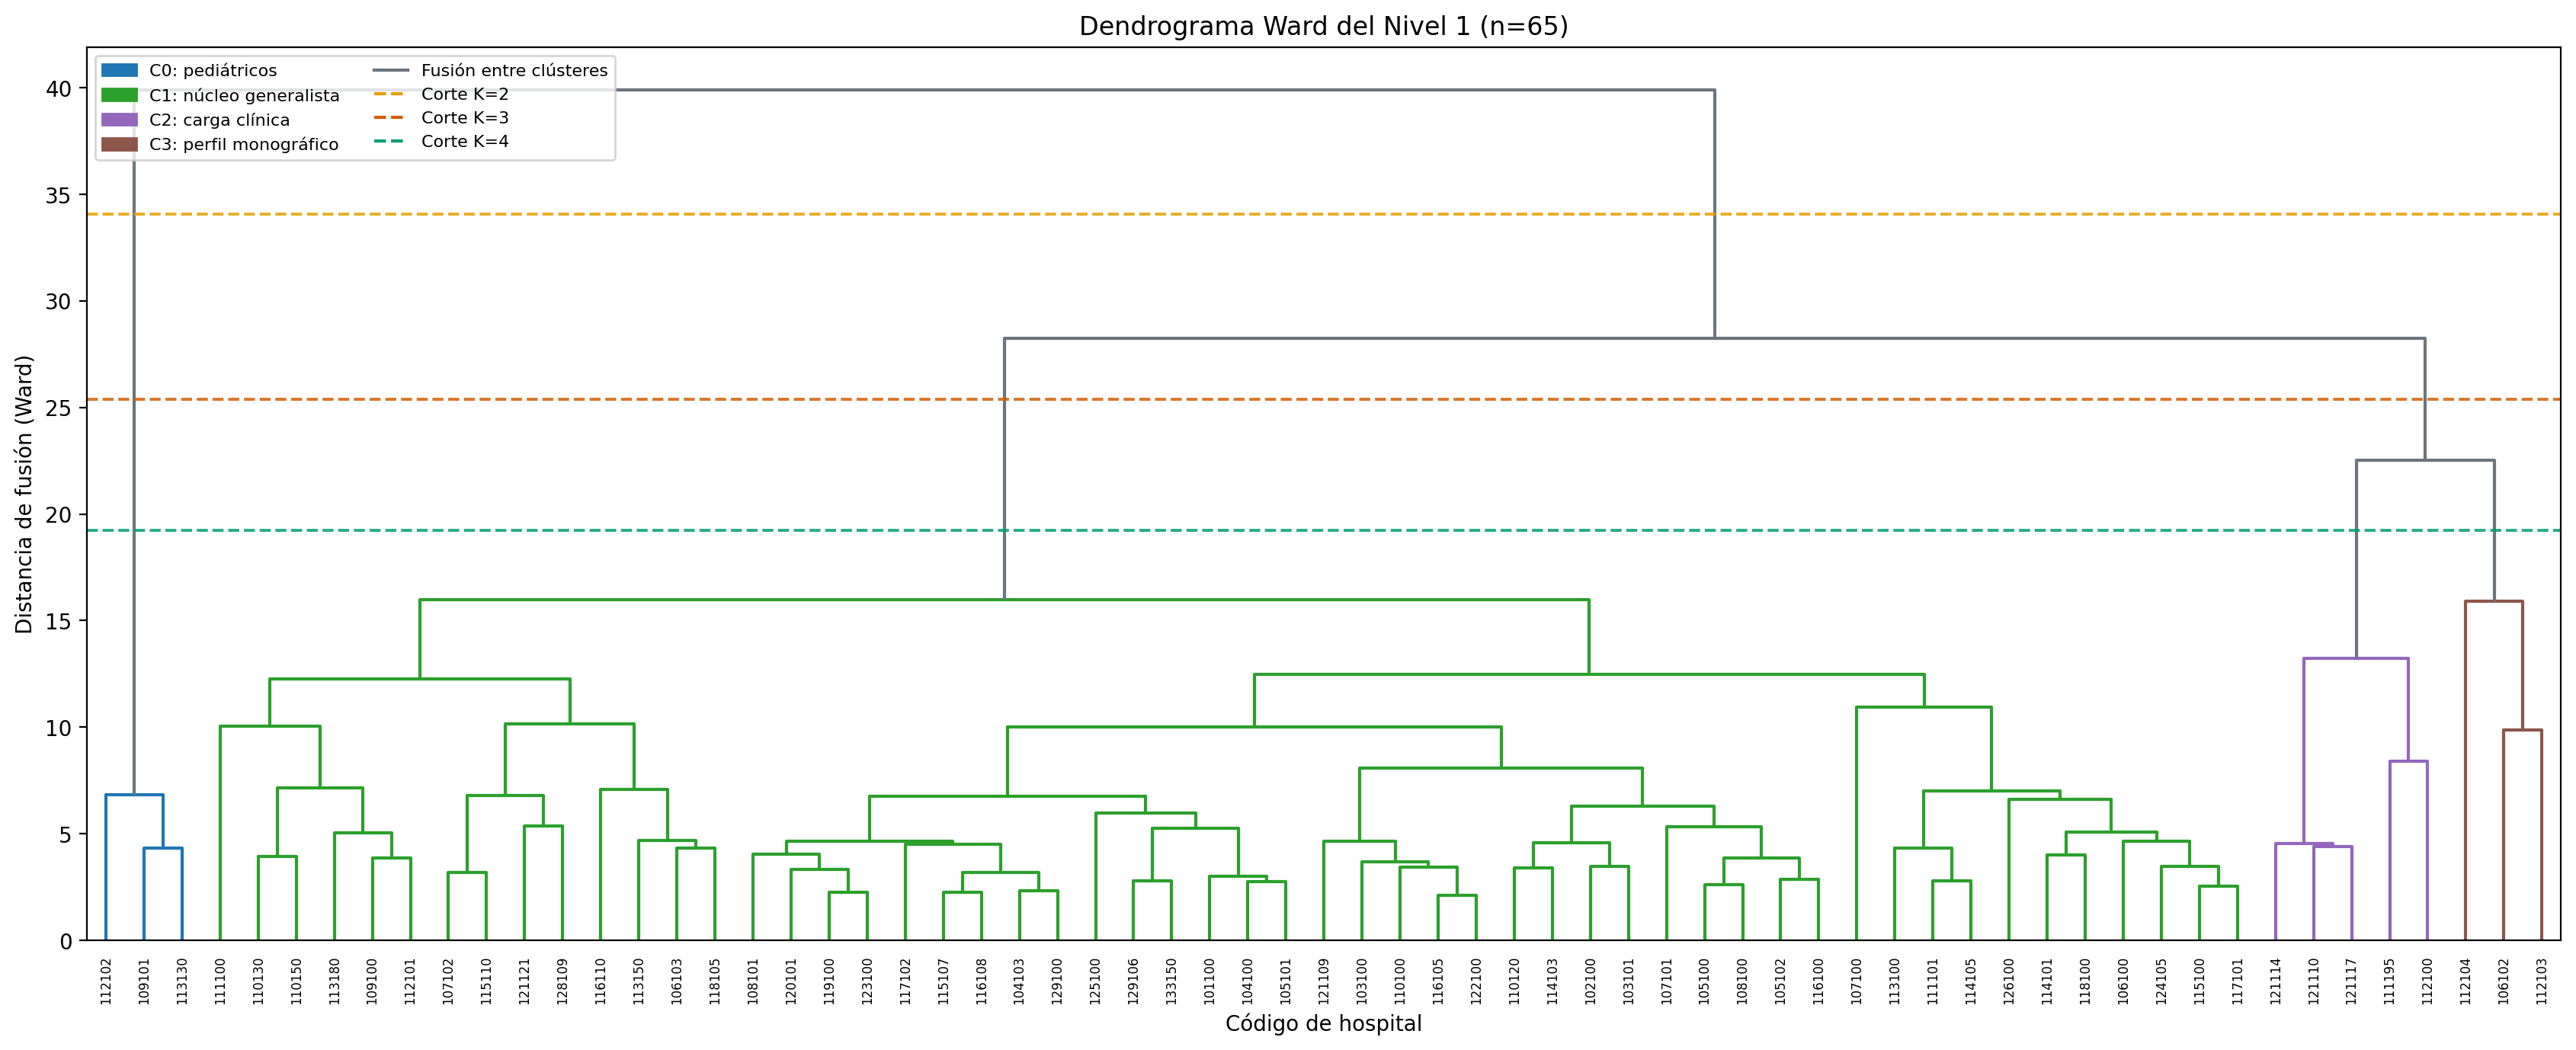
\includegraphics[width=\textwidth]{img/dendrograma_ward_nivel1.png}
\caption{Dendrograma de agrupamiento jerárquico global del Nivel 1 mediante
Ward aglomerativo. Los colores de las ramas identifican los cuatro clústeres de
la partición reportada ($K=4$). Las ramas grises corresponden a fusiones entre
clústeres. Las líneas discontinuas se ubican entre las alturas de fusión que
delimitan los cortes $K=2$, $K=3$ y $K=4$.}
\label{fig:dendrograma-global}
\end{figure}

Para caracterizar cuantitativamente los cuatro clústeres obtenidos, la
Tabla~\ref{tab:perfiles-nivel1} presenta las medianas de variables
clínico-operativas seleccionadas. Estas diferencias permiten describir los
perfiles antes de asignarles etiquetas funcionales.

\begin{table}[htbp]
\centering
\caption{Medianas de los perfiles funcionales de los clústeres del Nivel 1
($K=4$).}
\label{tab:perfiles-nivel1}
\begin{tabular}{l c c c c}
\toprule
\textbf{Variable} & \textbf{$C0$ ($n=3$)} & \textbf{$C1$ ($n=54$)} &
\textbf{$C2$ ($n=5$)} & \textbf{$C3$ ($n=3$)} \\
\midrule
Egresos por año & 7{,}115 & 13{,}124 & 4{,}627 & 4{,}038 \\
Estancia media (días) & 6{,}1 & 6{,}8 & 8{,}7 & 8{,}7 \\
Peso medio GRD & 1{,}202 & 0{,}947 & 0{,}943 & 1{,}874 \\
Entropía GRD (índice 0--1) & 0{,}789 & 0{,}821 & 0{,}832 & 0{,}775 \\
Severidad media & 1{,}949 & 1{,}666 & 1{,}908 & 1{,}892 \\
Comorbilidades promedio & 3{,}68 & 4{,}45 & 5{,}52 & 6{,}00 \\
Tasa de CMA & 13{,}5\% & 14{,}4\% & 34{,}8\% & 0{,}0\% \\
Egresos pediátricos & 95{,}4\% & 14{,}2\% & 2{,}5\% & 0{,}0\% \\
Egresos geriátricos & 0{,}0\% & 25{,}6\% & 37{,}2\% & 46{,}0\% \\
Ingresos obstétricos & 0{,}0\% & 20{,}0\% & 10{,}5\% & 0{,}0\% \\
Proporción de egresos neonatales & 0{,}0\% & 2{,}8\% & 0{,}461\% & 0{,}0\% \\
Edad mediana (años) & 5{,}0 & 41{,}8 & 56{,}8 & 63{,}6 \\
\bottomrule
\end{tabular}
\end{table}

La interpretación de los perfiles de la Tabla~\ref{tab:perfiles-nivel1} permite
caracterizar empíricamente cada grupo y, a partir de esa evidencia, derivar una
etiqueta funcional descriptiva de forma posterior al agrupamiento. El algoritmo
no recibió nombres ni categorías funcionales durante la construcción de la
partición.

\begin{itemize}
    \item \textbf{Clúster $C0$ ($n=3$): Hospitales Pediátricos.} Concentra
    prácticamente la totalidad de sus egresos en población pediátrica
    ($95{,}4\%$) y registra una edad mediana de ingreso de $5{,}0$ años, con
    actividad geriátrica y obstétrica nula. El peso medio GRD ($1{,}202$) y la
    severidad media ($1{,}949$) reflejan la complejidad de las especialidades
    infantiles. Está integrado por el Hospital Clínico de Niños Dr.\ Roberto del
    Río, el Hospital de Niños Dr.\ Luis Calvo Mackenna y el Hospital Dr.\
    Exequiel González Cortés.

    \item \textbf{Clúster $C3$ ($n=3$): grupo de especialización clínica
    heterogénea.} Registra el peso medio GRD más alto entre los cuatro perfiles
    (mediana $1{,}874$), la mayor edad mediana de la red ($63{,}6$ años), una
    estancia media de $8{,}7$ días y actividad obstétrica, pediátrica y CMA
    nula. Integra al Instituto Nacional de Enfermedades Respiratorias y Cirugía
    Torácica (INER), al Instituto de Neurocirugía Dr.\ Alfonso Asenjo y al
    Hospital Dr.\ Eduardo Pereira Ramírez de Valparaíso. Los dos primeros son
    establecimientos especializados, mientras que el tercero es un hospital
    general. Los coeficientes Silhouette individuales son $0{,}270$ para INER,
    $0{,}053$ para el Instituto de Neurocirugía y $-0{,}173$ para el Hospital
    Eduardo Pereira. Este último también cumple los tres criterios de atipicidad
    combinados (Sección~\ref{sec:res-outliers-combinados}), por lo que su
    asignación a $C3$ debe interpretarse como ambigua. En consecuencia, la
    etiqueta describe un patrón de especialización clínica del grupo, sin
    atribuir carácter monográfico al conjunto de sus tres establecimientos.

    \item \textbf{Clúster $C2$ ($n=5$): grupo de carga clínica heterogénea.}
    Comparte con $C3$ una estancia media prolongada ($8{,}7$ días) y una
    población de mayor edad (edad mediana $56{,}8$ años; $37{,}2\%$ de egresos
    geriátricos), pero su peso medio GRD ($0{,}943$) es cercano al del núcleo
    generalista. Destaca por una mediana de comorbilidades superior a la del
    núcleo ($5{,}52$ frente a $4{,}45$) y por una tasa de CMA heterogénea, cuya
    mediana es $34{,}8\%$. Está integrado por el HUAP Dr.\ Alejandro del Río,
    el Hospital Del Salvador, el Hospital Dr.\ Abraham Godoy de Lautaro, el
    Hospital Intercultural de Nueva Imperial y el Hospital de Pitrufquén.

    El grupo reúne hospitales de escala y localización distintas. Por ejemplo,
    el HUAP presenta una tasa de CMA de $0{,}1\%$, coherente con su función de
    urgencia y trauma de alta complejidad, mientras que el Hospital Dr.\ Abraham
    Godoy alcanza $41{,}6\%$. Esta heterogeneidad hace preferible mantener la
    denominación descriptiva $C2$, sin imponer una etiqueta funcional breve que
    simplifique en exceso a sus cinco integrantes.

    \item \textbf{Clúster $C1$ ($n=54$): Núcleo Generalista.} Es el grupo
    mayoritario de hospitales generales de la red pública. Presenta una mediana
    de 13.124 egresos anuales, estancia media de $6{,}8$ días, peso medio GRD de $0{,}947$ y una composición asistencial mixta, con $14{,}2\%$ de egresos pediátricos, $25{,}6\%$ de egresos geriátricos, $20{,}0\%$ de ingresos obstétricos y una proporción de egresos neonatales de $2{,}8\%$. La diversidad y el equilibrio relativo de su actividad
    permiten describirlo como el Núcleo Generalista de la red.
\end{itemize}

La proyección bidimensional mediante componentes principales de la
Figura~\ref{fig:pca-nivel1} ilustra la disposición de los hospitales en las dos
primeras componentes principales para las soluciones $K=2$, $K=3$ y $K=4$. Esta
proyección facilita examinar visualmente la separación de los establecimientos
especializados respecto del núcleo generalista, pero no constituye una prueba
adicional de validez del clustering.

\begin{figure}[htbp]
\centering
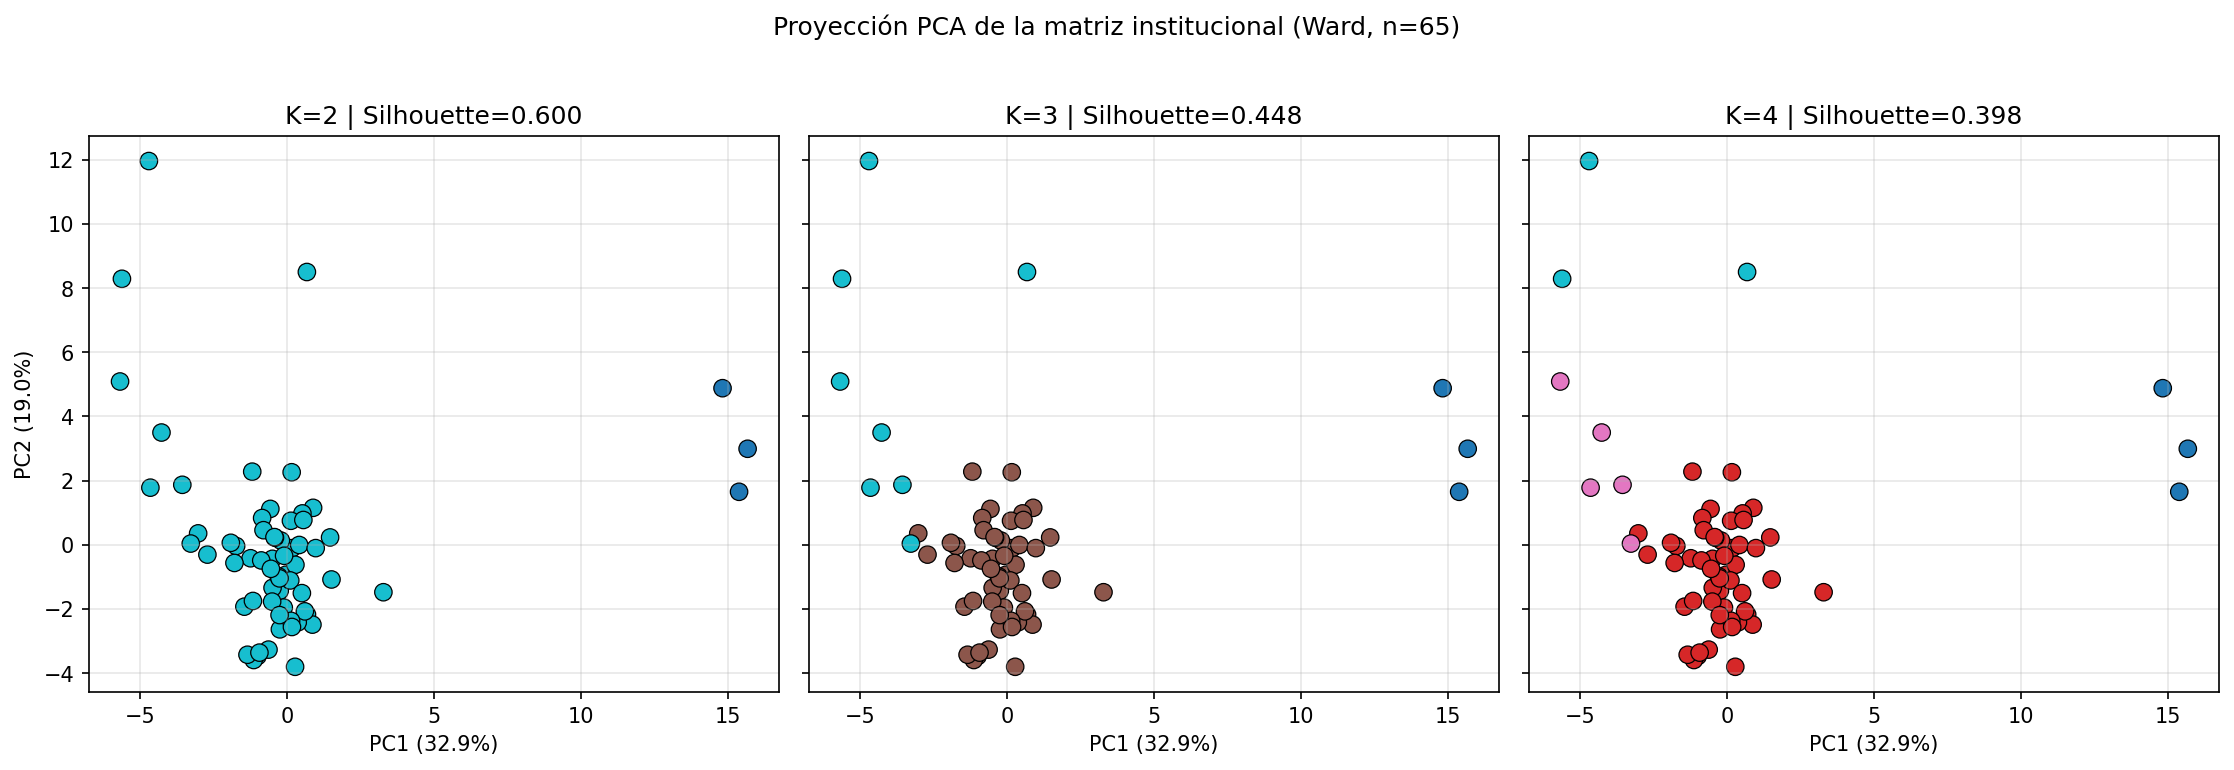
\includegraphics[width=\textwidth]{img/pca_particiones_nivel1.png}
\caption{Proyecciones bidimensionales PCA de la matriz institucional para las
soluciones Ward con $K=2$, $K=3$ y $K=4$. Los valores de Silhouette mostrados
corresponden a cada partición.}
\label{fig:pca-nivel1}
\end{figure}


\section{Subtipología exploratoria del bloque generalista (nivel 2)}
\label{sec:nivel2}

Dado que el clúster $C1$ concentra 54 de los 65 hospitales
($83{,}1\%$ del sistema), se aplicó un segundo nivel de clustering sobre este
subconjunto, de acuerdo con el diseño descrito en la
Sección~\ref{sec:nivel2-metodo}. Al operar sobre un subconjunto de hospitales,
esta subdivisión tiene un carácter exploratorio: su propósito no es establecer
fronteras funcionales equivalentes a las del Nivel~1, sino describir posibles
gradientes de volumen, complejidad y orientación clínica dentro del núcleo
generalista.

La búsqueda de configuraciones para
$K_{sub}\in\{2,3,\ldots,10\}$ se presenta en la
Tabla~\ref{tab:metricas-nivel2}. Además de las métricas internas, se reportan
los tamaños de grupo, la cantidad de grupos unitarios y el número de
subclústeres con al menos cuatro hospitales.

\begin{table}[htbp]
\centering
\caption{Búsqueda de subclústeres Ward en el núcleo generalista (Nivel~2, $n=54$).}
\label{tab:metricas-nivel2}

\begin{tabular}{c c c c c c l}
\toprule
\textbf{$K_{sub}$} & \textbf{Silhouette} & \textbf{Davies--Bouldin} & \textbf{Unitarios} & \textbf{Pares} & \textbf{$n\geq4$} & \textbf{Tamaños} \\
\midrule
2 & 0,193 & 2,303 & 0 & 0 & 2 & 40, 14 \\
3 & 0,113 & 2,282 & 0 & 0 & 3 & 29, 14, 11 \\
4 & 0,129 & 1,957 & 0 & 0 & 4 & 29, 11, 8, 6 \\
5 & 0,122 & 1,583 & 1 & 0 & 4 & 29, 10, 8, 6, 1 \\
6 & 0,132 & 1,486 & 1 & 0 & 5 & 29, 10, 6, 4, 4, 1 \\
7 & 0,136 & 1,285 & 2 & 0 & 5 & 29, 10, 5, 4, 4, 1, 1 \\
8 & 0,111 & 1,423 & 2 & 0 & 6 & 15, 14, 10, 5, 4, 4, 1, 1 \\
\textbf{9} & \textbf{0,101} & \textbf{1,368} & \textbf{2} & \textbf{0} & \textbf{7} & \textbf{15, 10, 9, 5, 5, 4, 4, 1, 1} \\
10 & 0,109 & 1,294 & 2 & 1 & 6 & 15, 10, 9, 5, 4, 4, 3, 2, 1, 1 \\
\bottomrule
\end{tabular}
\end{table}

Para evaluar si estas divisiones se reproducen al perturbar la muestra, se
aplicó al Nivel~2 el mismo protocolo de 100 submuestras sin reposición empleado
para el Nivel~1. En cada réplica se seleccionaron 43 de los 54 hospitales,
se ajustó nuevamente el preprocesamiento y se aplicó Ward. La Tabla~\ref{tab:estabilidad-nivel2}
resume la concordancia con la partición de referencia para $K_{sub}=2$, $3$ y
$9$.

\begin{table}[htbp]
\centering
\caption{Estabilidad de la partición Ward por submuestreo, Nivel~2 (100 réplicas).}
\label{tab:estabilidad-nivel2}
\begin{tabular}{c c c c}
\toprule
\textbf{$K_{sub}$} & \textbf{Silhouette original} & \textbf{ARI mediano [P2,5; P97,5]} & \textbf{NMI mediano [P2,5; P97,5]} \\
\midrule
2 & 0,193 & 0,526 [0,022; 1,000] & 0,456 [0,035; 1,000] \\
3 & 0,113 & 0,475 [0,127; 0,835] & 0,538 [0,277; 0,814] \\
9 & 0,101 & 0,559 [0,353; 0,840] & 0,774 [0,664; 0,919] \\
\bottomrule
\end{tabular}
\end{table}

La solución con dos grupos tiene el mayor Silhouette del barrido, pero su ARI
mediano de 0,526 sigue lejos de la estabilidad del Nivel~1 (ARI mediano
0,958). La solución de nueve grupos tampoco reproduce una tipología robusta:
aunque su NMI es mayor, su ARI mediano es 0,559, y contiene dos subgrupos
unitarios. En consecuencia, el Nivel~2 se limita en el cuerpo del texto a una
separación exploratoria amplia en dos bloques de 40 y 14 hospitales, por lo que no se
sostienen nueve perfiles funcionales generalizables. La asignación de nueve
subgrupos y sus perfiles descriptivos se conserva en el Anexo como material
suplementario.

Los casos $S1$ (Hospital Clínico San Borja--Arriarán) y $S8$ (Hospital Dr. Gustavo
Fricke) de la solución suplementaria son observaciones unitarias alejadas del
centroide del núcleo, no subtipos funcionales. Por tanto, no se usan para
inferencias ni para etiquetar categorías hospitalarias.

\section{Estabilidad de la partición mediante submuestreo}
\label{sec:res-estabilidad}

Siguiendo el procedimiento descrito en la Sección~\ref{sec:bootstrap}, se ejecutaron 100 iteraciones de submuestreo sin reposición. En cada réplica se seleccionó el $80\,\%$ de los 65 hospitales ($n_{\text{sub}}=52$), se recalculó el preprocesamiento y se aplicó clustering jerárquico Ward con $K=4$. La Tabla~\ref{tab:estabilidad-global} presenta los intervalos percentilares empíricos (percentiles 2{,}5 y 97{,}5) del coeficiente Silhouette de cada submuestra y de la concordancia entre su partición y la asignación original, medida mediante ARI y NMI.

\begin{table}[htbp]
\centering
\caption{Estabilidad global de la partición Ward $K=4$ por submuestreo (100 réplicas del 80\,\%).}
\label{tab:estabilidad-global}
\begin{tabular}{l c c c}
\toprule
\textbf{Métrica} & \textbf{Mediana} & \textbf{Percentil 2,5} &
\textbf{Percentil 97,5} \\
\midrule
Silhouette & 0,395 & 0,225 & 0,460 \\
ARI vs. partición original & 0,958 & 0,514 & 1,000 \\
NMI vs. partición original & 0,917 & 0,656 & 1,000 \\
\bottomrule
\end{tabular}
\end{table}

La mediana del Silhouette en las submuestras ($0{,}395$) es cercana al valor obtenido para la partición completa de 65 hospitales ($0{,}401$). Por tanto, la estructura de cohesión y separación observada en la solución principal se reproduce habitualmente al retirar una fracción de los establecimientos. No obstante, el intervalo percentilar $[0{,}225;\,0{,}460]$ muestra que la calidad interna de la partición varía entre réplicas. Algunas submuestras
producen agrupamientos menos compactos que la solución calculada sobre el conjunto completo.

La concordancia con la partición original es alta en la réplica típica, pues las medianas de ARI y NMI alcanzan $0{,}958$ y $0{,}917$, respectivamente. Sin embargo, los percentiles inferiores de ambas métricas (ARI $=0{,}514$ y NMI $=0{,}656$) indican que existen submuestras en las que la composición de los grupos se modifica en mayor medida. En consecuencia, los resultados respaldan una estructura global generalmente reproducible, pero no implican que la pertenencia de todos los hospitales a su clúster se conserve con la misma consistencia en cada submuestra.

Para localizar esta variabilidad, la Tabla~\ref{tab:estabilidad-grupo} desagrega la estabilidad por clúster mediante dos indicadores. La estabilidad individual promedio corresponde a la coasignación media de cada hospital con los demás integrantes de su clúster original, condicionada a las réplicas en que ambos hospitales fueron seleccionados. El índice de Jaccard promedio cuantifica el solapamiento entre los integrantes originales de cada clúster presentes en una submuestra y el grupo de dicha réplica con el que presentan mayor coincidencia.

\begin{table}[htbp]
\centering
\caption{Estabilidad de la partición desagregada por clúster del Nivel 1 (100 submuestras).}
\label{tab:estabilidad-grupo}
\begin{tabular}{l c c c}
\toprule
\textbf{Clúster} & \textbf{$n$} &
\textbf{Estabilidad individual (media)} &
\textbf{Jaccard promedio} \\
\midrule
$C0$ (pediátricos) & 3 & 1,000 & 1,000 \\
$C1$ (núcleo generalista) & 54 & 0,946 & 0,967 \\
$C2$ (perfil de carga clínica) & 5 & 0,967 & 0,791 \\
$C3$ (perfil monográfico) & 3 & 0,911 & 0,904 \\
\bottomrule
\end{tabular}
\end{table}

El clúster pediátrico $C0$ presenta coasignación y solapamiento perfectos en las 100 réplicas, lo que es consistente con su perfil clínico claramente diferenciado respecto del resto de la red. El núcleo generalista $C1$, que reúne 54 hospitales, también muestra una elevada estabilidad conjunta: su Jaccard promedio es $0{,}967$ y su estabilidad individual media alcanza $0{,}946$. Así, la mayor parte de los hospitales generalistas conserva su relación de proximidad con los demás integrantes del núcleo al modificar la muestra de análisis.

El clúster $C2$ registra la mayor estabilidad individual promedio entre los grupos no pediátricos ($0{,}967$), aunque su Jaccard promedio es el menor de la partición ($0{,}791$). Esto señala que sus hospitales tienden a mantener una alta coasignación con sus pares originales cuando son seleccionados, pero que la composición completa del grupo es más sensible a la omisión de algunos establecimientos en las submuestras. Esta sensibilidad es coherente con el tamaño reducido del clúster ($n=5$), pues la exclusión de uno o más de sus integrantes altera proporcionalmente su composición en mayor medida que en el núcleo generalista.

Por su parte, el clúster monográfico $C3$ presenta estabilidad individual media de $0{,}911$ y un Jaccard promedio de $0{,}904$. Ambos valores son inferiores a los observados en $C0$ y $C1$, pero no permiten caracterizar a $C3$ como un grupo inestable, pues en la mayoría de
las réplicas sus tres hospitales conservan una asociación reconocible. En conjunto, el submuestreo muestra que la partición de Nivel~1 es predominantemente reproducible, aunque la estabilidad de los grupos pequeños y la asignación de algunos establecimientos específicos dependen en mayor medida de la composición de la muestra analizada. Estos resultados constituyen evidencia de sensibilidad interna del procedimiento y deben interpretarse junto con los análisis descriptivos, de sensibilidad temporal y de detección de observaciones atípicas presentados en las secciones precedentes.


\section{Validación estadística por variable}
\label{sec:res-validacion}

Siguiendo el procedimiento descrito en la Sección~\ref{sec:validacion-grupos},
se aplicó la prueba de Kruskal-Wallis ($\alpha=0{,}05$) a las 28 variables
originales en escala no transformada. Los $p$-valores se ajustaron mediante el
procedimiento de Benjamini-Hochberg (BH), con el propósito de controlar la tasa
de falsos descubrimientos al efectuar comparaciones simultáneas. Las variables
se ordenan según su tamaño de efecto $\varepsilon^2$, calculado mediante la
Ecuación~\ref{eq:epsilon2}, el cual cuantifica la magnitud de las diferencias
entre grupos.

Entre las variables evaluadas se incluye \texttt{peso\_medio\_cma}, que se
reporta de forma descriptiva y se incorpora a esta caracterización posterior al
agrupamiento. Sin embargo, dicho indicador fue excluido de la matriz utilizada
para construir los clústeres, debido a que no es comparable en establecimientos
sin actividad CMA, como se indicó en la Sección~\ref{sec:universo}.

Estos resultados deben interpretarse como una caracterización posterior al
agrupamiento. Dado que los clústeres se construyeron a partir de estas mismas
variables, la significancia estadística no constituye una validación
independiente de la partición. En cambio, permite identificar qué variables
presentan mayores diferencias entre los perfiles resultantes y ordenar su
contribución descriptiva mediante $\varepsilon^2$.

En el Nivel~1 (Tabla~\ref{tab:kruskal-nivel1}), 26 de las 28 variables
discriminan significativamente entre los cuatro clústeres después del ajuste
BH. Los mayores tamaños de efecto corresponden a \texttt{tasa\_partos}
($\varepsilon^2=0{,}395$), \texttt{edad\_mediana}
($\varepsilon^2=0{,}377$) y \texttt{pct\_obstetrica\_ingreso}
($\varepsilon^2=0{,}345$). Estos resultados son consistentes con la separación
entre el perfil pediátrico, los establecimientos de mayor especialización y los
hospitales generalistas, particularmente respecto de la composición etaria de
los egresos y de la actividad gineco-obstétrica.

Solo \texttt{cv\_estancia} y \texttt{pabellones\_promedio} no alcanzan significancia tras el ajuste BH. Esto indica que, bajo esta comparación y nivel de corrección, no se observa evidencia suficiente de diferencias sistemáticas entre los cuatro clústeres en la variabilidad relativa de la estancia ni en el número promedio de pabellones. No implica que estas variables sean idénticas entre grupos ni que carezcan de relevancia clínica individual.

\begin{table}[htbp]
\centering
\caption{Prueba de Kruskal-Wallis con corrección Benjamini-Hochberg, Nivel~1 ($K=4$, $n=65$).}
\label{tab:kruskal-nivel1}

\begin{tabular}{l c c c c c}
\toprule
\textbf{Variable} & \textbf{$H$} & \textbf{$p$-valor} &
\textbf{$p_{\text{BH}}$} & \textbf{$\varepsilon^2$} &
\textbf{Discrimina} \\
\midrule
tasa\_partos
& 27,1 & $5{,}62 \times 10^{-6}$ & $1{,}34 \times 10^{-4}$ & 0,395 & Sí \\
edad\_mediana
& 26,0 & $9{,}58 \times 10^{-6}$ & $1{,}34 \times 10^{-4}$ & 0,377 & Sí \\
pct\_obstetrica\_ingreso
& 24,0 & $2{,}45 \times 10^{-5}$ & $2{,}29 \times 10^{-4}$ & 0,345 & Sí \\
pct\_pediatrico
& 22,9 & $4{,}16 \times 10^{-5}$ & $2{,}92 \times 10^{-4}$ & 0,327 & Sí \\
pct\_femenino\_fertil
& 22,1 & $6{,}31 \times 10^{-5}$ & $3{,}53 \times 10^{-4}$ & 0,313 & Sí \\
tasa\_prematurez
& 20,5 & $1{,}31 \times 10^{-4}$ & $6{,}13 \times 10^{-4}$ & 0,287 & Sí \\
pct\_geriatrico
& 20,2 & $1{,}56 \times 10^{-4}$ & $6{,}22 \times 10^{-4}$ & 0,282 & Sí \\
severidad\_media
& 19,4 & $2{,}31 \times 10^{-4}$ & $7{,}24 \times 10^{-4}$ & 0,268 & Sí \\
mortalidad\_media
& 19,3 & $2{,}33 \times 10^{-4}$ & $7{,}24 \times 10^{-4}$ & 0,268 & Sí \\
pct\_alta\_domicilio
& 17,1 & $6{,}64 \times 10^{-4}$ & $1{,}86 \times 10^{-3}$ & 0,232 & Sí \\
pct\_urgencia
& 16,8 & $7{,}83 \times 10^{-4}$ & $1{,}99 \times 10^{-3}$ & 0,226 & Sí \\
estancia\_mediana
& 16,3 & $9{,}79 \times 10^{-4}$ & $2{,}28 \times 10^{-3}$ & 0,218 & Sí \\
egresos\_por\_anio
& 14,1 & $0{,}003$ & $0{,}006$ & 0,182 & Sí \\
peso\_medio\_grd
& 13,6 & $0{,}004$ & $0{,}007$ & 0,173 & Sí \\
pct\_programada
& 13,4 & $0{,}004$ & $0{,}007$ & 0,170 & Sí \\
pct\_alta\_fallecido
& 13,3 & $0{,}004$ & $0{,}007$ & 0,169 & Sí \\
estancia\_media
& 13,1 & $0{,}004$ & $0{,}007$ & 0,166 & Sí \\
comorbilidades\_promedio
& 12,9 & $0{,}005$ & $0{,}007$ & 0,163 & Sí \\
pct\_uso\_pabellon
& 12,6 & $0{,}006$ & $0{,}008$ & 0,157 & Sí \\
pct\_alta\_traslado
& 12,4 & $0{,}006$ & $0{,}008$ & 0,154 & Sí \\
peso\_medio\_cma
& 12,4 & $0{,}006$ & $0{,}008$ & 0,153 & Sí \\
pct\_estancia\_larga
& 11,8 & $0{,}008$ & $0{,}010$ & 0,144 & Sí \\
pct\_origen\_referencia
& 11,3 & $0{,}010$ & $0{,}012$ & 0,137 & Sí \\
tasa\_cma
& 10,7 & $0{,}014$ & $0{,}016$ & 0,126 & Sí \\
entropia\_grd
& 9,5 & $0{,}024$ & $0{,}026$ & 0,106 & Sí \\
pct\_origen\_emergencia
& 9,4 & $0{,}024$ & $0{,}026$ & 0,105 & Sí \\
cv\_estancia
& 5,5 & $0{,}139$ & $0{,}144$ & 0,041 & No \\
pabellones\_promedio
& 4,8 & $0{,}188$ & $0{,}188$ & 0,029 & No \\
\bottomrule
\end{tabular}
\end{table}

La circularidad asociada a esta caracterización se examinó mediante dos
nulas sobre el flujo completo descritas en la
Sección~\ref{sec:permutacion-circularidad}. La primera permutó de forma
independiente cada variable entre hospitales, preservando su distribución
marginal y eliminando la estructura conjunta. En 500 repeticiones, la mediana
del número de variables significativas fue 1, el percentil 95 fue 5 y el máximo
fue 10. Ninguna réplica alcanzó las 26 variables observadas. Este resultado
muestra que Ward no genera el patrón observado cuando se eliminan por completo
las dependencias entre variables.

La segunda nula simuló 500 matrices normales multivariadas con la media y
covarianza observadas después de las transformaciones y el escalado robusto. Al
preservar la dependencia lineal, esta referencia es más exigente: la mediana
fue 23 variables significativas, el percentil 95 fue 26 y el máximo fue 28. En
59 de 500 réplicas la nula igualó o superó las 26 variables observadas
($p_{\mathrm{emp}}=0{,}1198$, con corrección de continuidad). Por tanto, el
número de diferencias detectadas por Kruskal--Wallis no supera de forma
concluyente lo esperable de una geometría correlacionada sin una estructura de
grupos explícita. La Tabla~\ref{tab:nulas-circularidad} resume los resultados de
ambas nulas. Estas pruebas mantienen utilidad descriptiva para ordenar los
atributos que difieren en la partición obtenida, pero no aportan validación
independiente de los clústeres.

\begin{table}[htbp]
\centering
\caption{Nulas del flujo Ward $K=4$ y Kruskal--Wallis/BH: número de variables significativas de 28 evaluadas.}
\label{tab:nulas-circularidad}
\begin{tabular}{l c c c c}
\toprule
\textbf{Nula} & \textbf{Mediana} & \textbf{P95} & \textbf{Máximo} & \textbf{$p_{\mathrm{emp}}$} \\
\midrule
Permutación independiente por columna & 1 & 5 & 10 & $<0{,}002$ \\
Normal multivariada con covarianza preservada & 23 & 26 & 28 & 0,1198 \\
\bottomrule
\end{tabular}
\par\smallskip
\begin{minipage}{\textwidth}
\normalsize\raggedright
\textit{Nota.} Ambas nulas usan 500 réplicas. El valor observado fue 26. En la
segunda nula, la covarianza se preserva en esperanza, con un error relativo mediano
entre la covarianza muestral simulada y la observada de 0,308.
\end{minipage}
\end{table}

En el Nivel~2 (Tabla~\ref{tab:kruskal-nivel2}), el análisis se restringe a los 54 hospitales del núcleo generalista y compara los nueve subclústeres exploratorios ($S0$ a $S8$). De las 28 variables evaluadas, 24 presentan diferencias estadísticamente detectables entre subgrupos después del ajuste BH. Las seis con mayor tamaño de efecto corresponden a \texttt{peso\_medio\_grd}, \texttt{pct\_femenino\_fertil}, \texttt{pct\_obstetrica\_ingreso}, \texttt{entropia\_grd}, \texttt{pct\_estancia\_larga} y \texttt{tasa\_prematurez}.

En consecuencia, la subtipología exploratoria diferencia principalmente gradientes de complejidad clínica, composición de la casuística, permanencia hospitalaria y orientación obstétrica. Por tratarse de un segundo nivel exploratorio construido sobre el mismo conjunto de variables, los $p_{\text{BH}}$ no constituyen evidencia independiente de categorías externas o definitivas, de modo que su utilidad es descriptiva para ordenar los atributos que distinguen los perfiles obtenidos.

\begin{table}[htbp]
\centering
\caption{Variables con mayor tamaño de efecto, Kruskal--Wallis con corrección BH, Nivel~2 ($K_{sub}=9$, $n=54$).}
\label{tab:kruskal-nivel2}

\begin{tabular}{l c c c c}
\toprule
\textbf{Variable} & \textbf{$H$} & \textbf{$p$-valor} & \textbf{$p_{\text{BH}}$} & \textbf{$\varepsilon^2$} \\
\midrule
peso\_medio\_grd & 41,897 & $1{,}4158 \times 10^{-6}$ & $3{,}9642 \times 10^{-5}$ & 0,75327 \\
pct\_femenino\_fertil & 37,218 & $1{,}0493 \times 10^{-5}$ & 0,00014691 & 0,64929 \\
pct\_obstetrica\_ingreso & 35,751 & $1{,}9505 \times 10^{-5}$ & 0,00016808 & 0,61668 \\
entropia\_grd & 35,256 & $2{,}4011 \times 10^{-5}$ & 0,00016808 & 0,60570 \\
pct\_estancia\_larga & 34,309 & $3{,}5715 \times 10^{-5}$ & 0,00019920 & 0,58464 \\
tasa\_prematurez & 33,881 & $4{,}2686 \times 10^{-5}$ & 0,00019920 & 0,57514 \\
\bottomrule
\end{tabular}
\par\smallskip
\begin{minipage}{\textwidth}
\normalsize\raggedright
\textit{Nota.} Resultados ordenados de forma descendente por $\varepsilon^2$. La prueba caracteriza descriptivamente una partición exploratoria del Nivel~2 y no valida de forma independiente los subclústeres.
\end{minipage}
\end{table}

La magnitud de los tamaños de efecto debe considerarse junto con la significancia. Las seis variables resumidas en la Tabla~\ref{tab:kruskal-nivel2} son las que muestran las diferencias relativas más intensas entre los subgrupos. Este ordenamiento, sin embargo, no implica que las fronteras entre ellos sean robustas o generalizables.

Adicionalmente, se examinó la asociación entre la asignación de clústeres y la pertenencia a Servicios de Salud mediante una prueba de chi-cuadrado de independencia. En el Nivel~1 se obtuvo $\chi^2=65{,}329$ ($\text{gl}=84$, $p=0{,}935$), mientras que en el Nivel~2 se obtuvo $\chi^2=206{,}944$ ($\text{gl}=224$, $p=0{,}787$). En ambos niveles no se detectó una asociación estadísticamente significativa entre los clústeres y el Servicio de Salud.

Estas tablas de contingencia son dispersas, pues relacionan un número reducido de hospitales con numerosas categorías territoriales y administrativas. En consecuencia, el V de Cramér sin corrección puede sobreestimar la
asociación. Sus valores alcanzan $0{,}579$ en el Nivel~1 y $0{,}692$
en el Nivel~2. Al aplicar la corrección de sesgo de \citet{Bergsma2013}, el V de Cramér es aproximadamente cero en ambos niveles. Por ello, bajo esta especificación no se observa una asociación apreciable entre los clústeres y los Servicios de Salud. Este resultado no permite descartar de forma concluyente toda influencia territorial o administrativa, pero no aporta evidencia de que la segmentación obtenida esté determinada por dicha pertenencia.

\section{Comparación con la clasificación MINSAL}
\label{sec:res-minsal}

Siguiendo el procedimiento de contraste descrito en la
Sección~\ref{sec:contraste-minsal}, se comparó la partición de Nivel~1
($K=4$) con las categorías administrativas de complejidad del MINSAL
(Alta y Mediana Complejidad). La Tabla~\ref{tab:contingencia-minsal}
presenta la distribución de los 65 hospitales entre ambas clasificaciones.

\begin{table}[htbp]
\centering
\caption{Tabla de contingencia entre los clústeres del Nivel~1 y la clasificación administrativa MINSAL.}
\label{tab:contingencia-minsal}
\begin{tabular}{l c c c}
\toprule
\textbf{Clúster} & \textbf{Alta Complejidad} &
\textbf{Mediana Complejidad} & \textbf{Total} \\
\midrule
$C0$ (pediátricos) & 3 & 0 & 3 \\
$C1$ (núcleo generalista) & 47 & 7 & 54 \\
$C2$ (perfil de carga clínica) & 2 & 3 & 5 \\
$C3$ (especialización clínica heterogénea) & 3 & 0 & 3 \\
\bottomrule
\end{tabular}
\end{table}

Los índices globales de concordancia entre ambas particiones alcanzan un
Índice de Rand Ajustado (ARI) de $0{,}112$ y una Información Mutua
Normalizada (NMI) de $0{,}107$. Estos valores indican una concordancia global
baja entre la clasificación administrativa y la segmentación funcional
obtenida a partir de los egresos hospitalarios. Esta diferencia es consistente
con que ambas clasificaciones organizan los establecimientos mediante criterios
distintos. La clasificación MINSAL constituye una referencia administrativa,
mientras que los clústeres de este estudio se construyen a partir de la
producción, la complejidad clínica y la composición de la casuística observada
en los egresos.

La contingencia permite precisar cómo se distribuyen los perfiles funcionales
respecto de las categorías administrativas. Los tres hospitales pediátricos de
$C0$ y los tres establecimientos del grupo de especialización clínica
heterogénea $C3$ están clasificados por MINSAL como de Alta Complejidad. Esta
coincidencia describe la ubicación administrativa de los perfiles más
especializados identificados en el Nivel~1, sin constituir una validación externa
de la partición.

El núcleo generalista $C1$ concentra 47 hospitales de Alta Complejidad y 7 de
Mediana Complejidad. Por tanto, este perfil funcional reúne establecimientos
pertenecientes a ambas categorías administrativas, aunque predomina la Alta
Complejidad. De manera complementaria, el perfil de carga clínica $C2$ incluye
dos hospitales clasificados como de Alta Complejidad y tres como de Mediana
Complejidad. En consecuencia, ninguno de estos dos perfiles funcionales se
corresponde de manera exclusiva con una categoría administrativa MINSAL.

En conjunto, el contraste muestra que la clasificación administrativa no se
reproduce directamente al agrupar hospitales según sus características de
actividad clínica y casuística. Este resultado no permite establecer la
superioridad de una clasificación sobre la otra ni atribuir la diferencia a una
causa única. Más bien, evidencia que ambas particiones aportan lecturas
distintas y complementarias sobre la red hospitalaria pública.

\subsection{Comparación directa de homogeneidad interna}
\label{sec:res-homogeneidad}

El ARI y el NMI indican cuánto concuerdan dos particiones, pero no informan
directamente sobre su homogeneidad interna. Para comparar la compactación de los
grupos, se siguió el procedimiento descrito en la
Sección~\ref{sec:comparacion-homogeneidad}. El coeficiente Silhouette y la
dispersión intragrupo normalizada (WSS/TSS) se calcularon sobre la misma matriz
preprocesada de 35 variables empleada en el clustering. De forma
complementaria, la dispersión robusta se resumió mediante la desviación absoluta
mediana normalizada (MAD normalizado) sobre las 27 variables
clínico-operativas directas.

La Tabla~\ref{tab:homogeneidad-no-controlada} compara la solución Ward $K=4$
utilizada en este trabajo con la clasificación MINSAL. Un menor WSS/TSS y un
menor MAD normalizado indican menor dispersión dentro de los grupos.

\begin{table}[htbp]
\centering
\caption{Comparación de homogeneidad interna no controlada por número de grupos entre Ward $K=4$ y MINSAL.}
\label{tab:homogeneidad-no-controlada}
\begin{tabular}{l c c c c c}
\toprule
\textbf{Partición} & \textbf{$K$} & \textbf{Tamaños} &
\textbf{Silhouette} & \textbf{WSS/TSS} &
\textbf{MAD norm.} \\
\midrule
Ward $K=4$ & 4 & 3, 54, 5, 3 & 0,401 & 0,475 & 0,895 \\
MINSAL & 2 & 55, 10 & 0,070 & 0,944 & 0,999 \\
\bottomrule
\end{tabular}
\end{table}

En esta comparación no controlada, Ward $K=4$ presenta menor dispersión
intragrupo que MINSAL en las tres métricas. Sin embargo, esta primera
comparación debe interpretarse considerando que Ward utiliza cuatro grupos,
mientras que MINSAL contiene dos categorías. La fragmentación en un número
mayor de grupos puede reducir mecánicamente la dispersión intragrupo.

Por ello, la Tabla~\ref{tab:homogeneidad-controlada} repite el contraste con
Ward restringido a $K=2$, el mismo número de grupos de la clasificación MINSAL.
Ambas particiones se evalúan sobre la misma matriz y con las mismas métricas.

\begin{table}[htbp]
\centering
\caption{Comparación de homogeneidad interna controlada por número de grupos: Ward $K=2$ y MINSAL ($K=2$).}
\label{tab:homogeneidad-controlada}
\begin{tabular}{l c c c c c}
\toprule
\textbf{Partición} & \textbf{$K$} & \textbf{Tamaños} &
\textbf{Silhouette} & \textbf{WSS/TSS} &
\textbf{MAD norm.} \\
\midrule
Ward $K=2$ & 2 & 3, 62 & 0,605 & 0,707 & 0,931 \\
MINSAL & 2 & 55, 10 & 0,070 & 0,944 & 0,999 \\
\bottomrule
\end{tabular}
\end{table}

Incluso al fijar el número de grupos en $K=2$, la solución Ward presenta una
dispersión intragrupo menor que MINSAL y un Silhouette más alto. En este espacio
funcional, la separación entre los tres hospitales pediátricos y los 62
establecimientos restantes produce grupos más compactos que la partición
administrativa entre Alta y Mediana Complejidad.

La prueba de permutación evaluó si la dispersión intragrupo observada era menor
que la esperable bajo asignaciones aleatorias que preservan los tamaños de cada
partición. Se generaron 2.000 permutaciones para Ward $K=4$, Ward $K=2$ y
MINSAL. La Tabla~\ref{tab:permutacion-homogeneidad} resume los resultados.

\begin{table}[htbp]
\centering
\caption{Prueba de permutación de la dispersión intragrupo normalizada (2.000 reasignaciones).}
\label{tab:permutacion-homogeneidad}
\begin{tabular}{l c c c}
\toprule
\textbf{Partición} & \textbf{WSS/TSS observado} &
\textbf{$z$-score} & \textbf{$p$-valor empírico} \\
\midrule
Ward $K=4$ & 0,475 & $-20{,}97$ & $<0{,}001$ \\
Ward $K=2$ & 0,707 & $-20{,}98$ & $<0{,}001$ \\
MINSAL & 0,944 & $-4{,}68$ & 0,003 \\
\bottomrule
\end{tabular}
\par\smallskip
\begin{minipage}{\textwidth}
\normalsize\raggedright
\textit{Nota metodológica.} La distribución nula de WSS/TSS para MINSAL es marcadamente asimétrica (sesgo positivo): la mayor parte de las 2.000 permutaciones produce dispersiones intragrupo elevadas, con una cola derecha extendida. Esta asimetría es esperable en particiones muy desbalanceadas (grupos de 55 y 10 hospitales), donde la asignación aleatoria rara vez genera subconjuntos tan compactos como los observados. El $z$-score de $-4{,}68$ se calcula respecto de la media y desviación estándar de la distribución nula y no presupone normalidad, mientras que el $p$-valor empírico de $0{,}003$ indica que aproximadamente 6 de las 2.000 reasignaciones alcanzaron una dispersión igual o menor que la observada (WSS/TSS $= 0{,}944$). Este resultado confirma que la clasificación MINSAL presenta una compactación estadísticamente superior a la esperable por azar bajo sus propios tamaños de grupo, aunque notoriamente menor que la de las soluciones Ward.
\end{minipage}
\end{table}


Ninguna de las 2.000 particiones aleatorias para Ward $K=4$ o Ward $K=2$
alcanzó una dispersión intragrupo igual o menor que la observada. La
clasificación MINSAL también presenta una dispersión menor que la esperable bajo
asignaciones aleatorias con sus mismos tamaños de grupo, aunque con una
distancia menor respecto de su distribución nula.

Estos resultados describen la compactación interna de las particiones sobre la
matriz funcional completa. Sin embargo, Ward fue ajustado en ese mismo espacio,
por lo que sus menores valores de dispersión no constituyen una prueba
confirmatoria de mayor homogeneidad frente a MINSAL. La comparación se conserva
como diagnóstico descriptivo y se complementa a continuación con una evaluación
en bloques de variables no usados para construir las etiquetas Ward.

\subsection{Validación cruzada por bloques de variables}
\label{sec:res-homogeneidad-cruzada}

La Tabla~\ref{tab:homogeneidad-cruzada} evalúa cada partición en un bloque de
variables distinto del que se utilizó para construir Ward. Al agrupar con las 27
variables directas y evaluar sobre las 8 componentes de casuística, Ward $K=4$
obtuvo WSS/TSS $=0{,}616$, frente a $0{,}956$ para MINSAL, con una diferencia
MINSAL--Ward de $0{,}340$ (IC bootstrap 95\,\% $[0{,}176;0{,}540]$). En el
sentido inverso, al agrupar con componentes de casuística y evaluar sobre las
variables directas, Ward $K=4$ obtuvo WSS/TSS $=0{,}533$, frente a $0{,}940$
para MINSAL, con una diferencia de $0{,}407$ (IC 95\,\%
$[0{,}198;0{,}616]$). En ambas direcciones, la partición de cuatro grupos
conserva menor dispersión en el bloque retenido.

\begin{table}[htbp]
\centering
\caption{Validación cruzada de homogeneidad por bloques de variables. Ward se
ajusta solo en el bloque de agrupamiento y ambas particiones se evalúan en el
bloque retenido. La diferencia es $\mathrm{WSS/TSS}_{\mathrm{MINSAL}}-
\mathrm{WSS/TSS}_{\mathrm{Ward}}$; valores positivos favorecen menor dispersión
para Ward.}
\label{tab:homogeneidad-cruzada}

\begin{tabular}{l c c c c}
\toprule
\textbf{Bloque de agrupamiento} & \textbf{$K$ Ward} &
\textbf{WSS/TSS Ward} & \textbf{WSS/TSS MINSAL} &
\textbf{Diferencia (IC 95\,\%)} \\
\midrule
Directas $\rightarrow$ casuística & 4 & 0,616 & 0,956 &
0,340 $[0,176;0,540]$ \\
Casuística $\rightarrow$ directas & 4 & 0,533 & 0,940 &
0,407 $[0,198;0,616]$ \\
\addlinespace
Directas $\rightarrow$ casuística & 2 & 0,850 & 0,956 &
0,106 $[-0,057;0,262]$ \\
Casuística $\rightarrow$ directas & 2 & 0,740 & 0,940 &
0,200 $[-0,073;0,449]$ \\
\bottomrule
\end{tabular}
\par\smallskip
\begin{minipage}{\textwidth}
\normalsize\raggedright
\textit{Nota.} Los intervalos se obtuvieron mediante 5.000 remuestreos de los
65 hospitales. La evaluación cruzada por bloques no es independiente en sentido
temporal: ambos bloques derivan de los mismos establecimientos y período.
\end{minipage}
\end{table}

Al restringir Ward a $K=2$, para igualar el número de categorías de MINSAL, las
diferencias puntuales continúan siendo favorables a Ward, pero sus intervalos
bootstrap incluyen cero en ambas direcciones. Por tanto, esta evaluación no
entrega evidencia robusta de que Ward sea más homogéneo que MINSAL cuando se
controla simultáneamente la reutilización del espacio de evaluación y el número
de grupos. El resultado más acotado es que la solución Ward $K=4$ conserva una
compactación mayor en bloques retenidos, aunque parte de esa diferencia puede
asociarse a su mayor granularidad. En consecuencia, el estudio no establece una
superioridad general de la clasificación funcional sobre la administrativa, aunque sí
documenta que ambas organizan de manera distinta la actividad hospitalaria y que
los perfiles Ward muestran cohesión interna y estabilidad bajo las sensibilidades
reportadas.

\subsection{Discusión de los resultados frente a antecedentes nacionales e internacionales}
\label{sec:discusion-literatura}

La baja cohesión de la clasificación MINSAL observada en esta muestra es
congruente con la evidencia nacional previa. \citet{Giglio2021} reportaron
valores de Silhouette inferiores a $0{,}2$ para esa clasificación en los años
2014--2018, con casos negativos en algunos períodos. En este estudio, evaluada
sobre una matriz distinta, construida con registros GRD de 2019--2024 y solo con
hospitales de alta y mediana complejidad, la partición MINSAL alcanzó un
Silhouette de $0{,}070$. Los valores no son directamente intercambiables por las
diferencias de universo, período y variables, pero su coincidencia cualitativa
refuerza la conclusión acotada de que las etiquetas administrativas no capturan
por sí solas una estructura compacta de actividad clínica y casuística.

Los resultados también actualizan y matizan el hallazgo de \citet{Carlier2020},
quienes identificaron a la categoría de mediana complejidad como la menos
consistente entre años al intentar reproducir la clasificación administrativa
mediante indicadores de producción. En la presente partición, siete de los diez
hospitales MINSAL de mediana complejidad se integran al núcleo generalista $C1$,
junto con 47 hospitales de alta complejidad, los tres restantes se ubican en el
grupo $C2$, que también contiene dos hospitales de alta complejidad. Esta
distribución indica que las categorías administrativas no se corresponden de
forma exclusiva con los perfiles funcionales identificados. Sin embargo, no
permite atribuir la discrepancia a una categoría administrativa particular ni
comparar directamente la estabilidad temporal de ambos estudios, ya que sus
datos, variables y procedimientos de agrupamiento son distintos.

La comparación con el estudio francés de \citet{Chrusciel2021} muestra, a su
vez, que los ejes de organización funcional dependen de la información incluida
y del contexto de red. Ese trabajo identificó tres grupos principalmente
asociados con tamaño, diversidad y movilidad de pacientes. En esta tesis, la
solución de cuatro grupos distingue un núcleo generalista y perfiles pediátrico,
monográfico y de carga clínica heterogénea. La composición
demográfico-obstétrica aporta el $37{,}1\,\%$ de la distancia total, aunque la
partición se conserva en gran medida al excluir ese bloque ($ARI=0{,}933$).
Por tanto, la estructura chilena estudiada no se explica solo por la composición
de la demanda, pero esta dimensión participa más explícitamente que en el diseño
francés. La diferencia no contradice el antecedente internacional, ilustra que
las tipologías obtenidas son sensibles a las variables disponibles y que no
corresponde trasladar un número de grupos ni etiquetas funcionales entre redes
sin una evaluación contextual.

En conjunto, los tres antecedentes sitúan el aporte de esta investigación como una
actualización reproducible de la caracterización funcional de hospitales
chilenos con datos GRD recientes. La evidencia respalda la utilidad descriptiva
de complementar las categorías administrativas con información de producción y
casuística, pero no valida una tipología universal ni justifica usar la
partición Ward como criterio único para decisiones de financiamiento, desempeño
o asignación de recursos.

\subsection{Regresión LASSO: variables clínicas asociadas a la etiqueta MINSAL}
\label{sec:res-lasso}

El contraste anterior cuantifica la concordancia y la homogeneidad interna de
las particiones, pero no identifica qué variables de actividad clínica se
asocian con la clasificación administrativa. Para explorar esta relación, se
ajustó una regresión logística LASSO con penalización $L_1$ ($C=0{,}5$). La
variable objetivo fue el Nivel de Complejidad MINSAL, codificado como Alta
Complejidad $=1$ y Mediana Complejidad $=0$.

El modelo utilizó 27 variables clínico-operativas directas sobre los 65
hospitales, excluyendo las ocho componentes PCA de casuística y el indicador
\texttt{peso\_medio\_cma}. Esta exclusión mantiene la consistencia con la
matriz de clustering, pues \texttt{peso\_medio\_cma} no es comparable cuando un
establecimiento no registra actividad CMA.

La selección se evaluó mediante validación cruzada estratificada de cinco
pliegues. El procedimiento retuvo un máximo de ocho variables con mayor
frecuencia de selección. La Tabla~\ref{tab:lasso-frecuencia} presenta las ocho
variables retenidas y sus coeficientes en el modelo final ajustado sobre la
muestra completa.

\begin{table}[htbp]
\centering
\caption{Variables retenidas por LASSO: frecuencia de selección y coeficiente del modelo final.}
\label{tab:lasso-frecuencia}
\begin{tabular}{l c c}
\toprule
\textbf{Variable} & \textbf{Frecuencia de selección} &
\textbf{Coeficiente final} \\
\midrule
egresos\_por\_anio & 1,00 & 1,566 \\
pct\_estancia\_larga & 1,00 & 0,267 \\
pct\_alta\_traslado & 1,00 & $-0{,}567$ \\
pct\_femenino\_fertil & 0,80 & $-0{,}382$ \\
pct\_uso\_pabellon & 0,80 & 0,281 \\
tasa\_prematurez & 0,60 & 0,040 \\
cv\_estancia & 0,60 & 0,075 \\
comorbilidades\_promedio & 0,60 & $-0{,}103$ \\
\bottomrule
\end{tabular}
\end{table}

Las tres variables seleccionadas en todos los pliegues fueron
\texttt{egresos\_por\_anio}, \texttt{pct\_estancia\_larga} y
\texttt{pct\_alta\_traslado}. En el modelo final, \texttt{egresos\_por\_anio}
presenta el coeficiente estandarizado de mayor magnitud positiva. Dentro de este
modelo y esta muestra, un mayor volumen anual de egresos se asocia con una mayor
probabilidad estimada de pertenecer a la categoría de Alta Complejidad MINSAL.

Las demás variables retenidas muestran asociaciones condicionales de menor
magnitud. El signo negativo de \texttt{pct\_alta\_traslado} indica que, al
controlar por las demás variables del modelo, una mayor proporción de traslados
se asocia con una menor probabilidad estimada de Alta Complejidad. Estos
coeficientes describen asociaciones predictivas dentro de la muestra y no deben
interpretarse como efectos causales ni como criterios utilizados directamente
por MINSAL para asignar sus categorías.

Nueve variables alcanzaron una frecuencia de selección igual o superior a
$0{,}60$. Sin embargo, el procedimiento limita la selección a ocho variables,
por lo que \texttt{peso\_medio\_grd}, también seleccionado en tres de los cinco
pliegues, no fue retenido dentro del máximo establecido. Esta restricción evita
incrementar el número de predictores en una muestra con solo 65 hospitales.

El desempeño predictivo se evaluó fuera de muestra mediante la misma validación
cruzada estratificada de cinco pliegues. La Tabla~\ref{tab:lasso-desempeno}
presenta los resultados por pliegue.

\begin{table}[htbp]
\centering
\caption{Desempeño fuera de muestra del modelo LASSO (validación cruzada estratificada, 5 pliegues).}
\label{tab:lasso-desempeno}
\begin{tabular}{c c c c}
\toprule
\textbf{Pliegue} & \textbf{$n$ de prueba} &
\textbf{Accuracy} & \textbf{AUC} \\
\midrule
0 & 13 & 0,846 & 1,000 \\
1 & 13 & 0,846 & 1,000 \\
2 & 13 & 0,923 & 1,000 \\
3 & 13 & 1,000 & 1,000 \\
4 & 13 & 0,846 & 0,909 \\
\midrule
Promedio & -- & 0,892 & 0,982 \\
Baseline de clase mayoritaria & -- & 0,846 & -- \\
\bottomrule
\end{tabular}
\end{table}

La exactitud media del modelo alcanza $0{,}892$, mientras que un clasificador
que asignara siempre la categoría mayoritaria alcanzaría $0{,}846$. El AUC
medio es $0{,}982$. Estos resultados indican que las variables incluidas en el
modelo contienen información para discriminar, dentro de esta muestra, entre
las categorías administrativas de Alta y Mediana Complejidad.

Sin embargo, la interpretación debe reconocer el tamaño reducido y el
desbalance de la clase minoritaria. Solo 10 hospitales pertenecen a la categoría
de Mediana Complejidad, de modo que cada pliegue de prueba contiene dos
establecimientos de esa categoría. Por ello, las métricas de validación cruzada
deben leerse como evidencia exploratoria de capacidad discriminante y no como
una estimación definitiva del desempeño en otras poblaciones hospitalarias.

En conjunto, la regresión LASSO complementa la baja concordancia global entre la
segmentación funcional y MINSAL. El análisis identifica un conjunto reducido de
variables de actividad asociadas a la etiqueta administrativa en esta muestra,
entre las cuales el volumen anual de egresos presenta la asociación positiva de
mayor magnitud. Esto no implica que la clasificación MINSAL dependa únicamente
del volumen ni que sea insensible a otros atributos institucionales. Más bien,
muestra que la clasificación administrativa y la segmentación funcional basada
en casuística describen dimensiones relacionadas, pero no equivalentes, de la
red hospitalaria.


\section{Hospitales atípicos}

\label{sec:res-outliers}

\subsection{Influencia de las marcas globales antes del clustering}
\label{sec:res-outliers-preclustering}

Como prueba de sensibilidad previa, Isolation Forest se ajustó globalmente
sobre los 65 hospitales antes de construir Ward. Con contaminación $=10\,\%$
marcó siete establecimientos. Al excluirlos temporalmente y re-estimar Ward
$K=4$ sobre los 58 restantes, el Silhouette disminuyó de $0{,}401$ a $0{,}181$
y la concordancia con la partición base, restringida a los hospitales retenidos,
fue baja ($ARI=0{,}265$; $NMI=0{,}506$). Al reasignar las siete marcas al
centroide más próximo de la solución entrenada sin ellas, la concordancia sobre
los 65 hospitales se mantuvo baja ($ARI=0{,}317$; $NMI=0{,}500$) y el
Silhouette fue $0{,}154$.

Las marcas incluyen dos hospitales pediátricos, los tres miembros del grupo
$C3$ y dos hospitales de $C2$. Por tanto, la exclusión no elimina ruido aislado:
retira perfiles especializados que participan en la estructura que el análisis
pretende describir. La solución sin marcas fragmenta el núcleo en grupos de 16
y 38 hospitales y produce un grupo unitario. En consecuencia, la partición
principal conserva los 65 establecimientos. Isolation Forest se interpreta como
una señal de influencia global y no como un criterio de eliminación automática, por lo que
los criterios posteriores permiten caracterizar con mayor detalle los casos
alejados o con asignación ambigua.

\subsection{Sensibilidad al parámetro de contaminación de Isolation Forest}

\label{sec:res-outliers-sensibilidad}

Como se indicó en la Sección~\ref{sec:outliers-metodo}, el parámetro de contaminación de Isolation Forest determina la proporción aproximada de observaciones que el algoritmo tratará como potencialmente atípicas. Por ello, con contaminación $=10\,\%$ y un universo de 65 hospitales, se espera que el modelo marque aproximadamente entre 6 y 7 establecimientos. Este resultado depende parcialmente de la configuración seleccionada y no debe interpretarse, por sí solo, como una estimación independiente de la cantidad de hospitales atípicos en la red.

Para examinar esta dependencia, se ajustó Isolation Forest globalmente sobre los 65 hospitales y las 35 variables de la matriz institucional, utilizando niveles de contaminación de $5\,\%$, $10\,\%$, $15\,\%$ y $20\,\%$. La Tabla~\ref{tab:sensibilidad-contaminacion} presenta el número objetivo aproximado y el número de hospitales efectivamente marcados en cada configuración.

\begin{table}[htbp]
\centering
\caption{Sensibilidad de Isolation Forest, ajustado globalmente, al parámetro de contaminación.}
\label{tab:sensibilidad-contaminacion}
\begin{tabular}{c c c}
\toprule
\textbf{Contaminación} & \textbf{$n$ objetivo aproximado} & \textbf{$n$ marcado} \\
\midrule
5\,\%  & 3  & 4 \\
10\,\% & 6  & 7 \\
15\,\% & 10 & 10 \\
20\,\% & 13 & 13 \\
\bottomrule
\end{tabular}
\end{table}

El número de hospitales marcados aumenta al incrementar el parámetro de contaminación, en concordancia con el funcionamiento esperado del algoritmo. En consecuencia, la configuración con contaminación $=10\,\%$ se utiliza como una elección operativa para integrar los criterios de detección, y no como un umbral determinado exclusivamente por la estructura de los datos.

Cuatro establecimientos fueron marcados en los cuatro niveles de contaminación explorados: el Hospital Dr.\ Eduardo Pereira Ramírez, el Instituto Nacional de Enfermedades Respiratorias y Cirugía Torácica, el Instituto de Neurocirugía Dr.\ Alfonso Asenjo y el Hospital Dr.\ Exequiel González Cortés. Esta persistencia indica que dichos hospitales fueron identificados de forma consistente por Isolation Forest dentro del rango de parámetros evaluado. Sin embargo, no permite establecer por sí sola la naturaleza ni la causa de sus diferencias respecto de la red hospitalaria analizada.

\subsection{Criterios combinados y detección concordante}

\label{sec:res-outliers-combinados}

La detección combinó los tres criterios descritos en la Sección~\ref{sec:outliers-metodo}: Isolation Forest ajustado globalmente con contaminación $=10\,\%$, distancia al centroide del clúster normalizada mediante la MAD global y Silhouette individual negativo. Se consideraron como casos de detección concordante los hospitales que cumplieron al menos dos de estos criterios.

La Tabla~\ref{tab:outliers} presenta los nueve hospitales marcados por al menos un criterio. Tres de ellos cumplen dos o más criterios: el Hospital Dr.\ Eduardo Pereira Ramírez, el Instituto de Neurocirugía Dr.\ Alfonso Asenjo y el Hospital de Urgencia Asistencia Pública Dr.\ Alejandro del Río. Los seis establecimientos restantes fueron identificados por una sola medida, por lo que su señalamiento depende de ese criterio particular.

\begin{table}[htbp]
\centering
\caption{Hospitales marcados por al menos un criterio de detección de atipicidad.}
\label{tab:outliers}
\par\smallskip
\begin{minipage}{\textwidth}
\normalsize\raggedright
\textit{Nota.} Los establecimientos en negrita cumplen dos o más criterios de detección.
\end{minipage}

\renewcommand{\arraystretch}{1.15}
\begin{tabular}{p{5.4cm} c c p{5.3cm}}
\toprule
\textbf{Establecimiento} & \textbf{Clúster} & \textbf{$n$} & \textbf{Criterio(s)} \\
\midrule

\textbf{Hospital Dr.\ Eduardo Pereira Ramírez}
& $C3$ & 3 &
\textbf{Isolation Forest; distancia al centroide ($z_{\mathrm{MAD}}=3{,}316$); Silhouette $=-0{,}173$} \\

\textbf{Instituto de Neurocirugía Dr.\ Alfonso Asenjo}
& $C3$ & 3 &
\textbf{Isolation Forest; distancia al centroide ($z_{\mathrm{MAD}}=3{,}905$)} \\

\textbf{Hospital de Urgencia Asistencia Pública Dr.\ Alejandro del Río}
& $C2$ & 5 &
\textbf{Isolation Forest; distancia al centroide ($z_{\mathrm{MAD}}=3{,}257$)} \\

Instituto Nacional de Enfermedades Respiratorias y Cirugía Torácica
& $C3$ & 3 &
Isolation Forest \\

Hospital Dr.\ Exequiel González Cortés
& $C0$ & 3 &
Isolation Forest \\

Hospital de Niños Dr.\ Luis Calvo Mackenna
& $C0$ & 3 &
Isolation Forest \\

Hospital del Salvador
& $C2$ & 5 &
Isolation Forest \\

Hospital Clínico San Borja-Arriarán
& $C1$ & 54 &
Distancia al centroide ($z_{\mathrm{MAD}}=3{,}281$) \\

Hospital Dr.\ Gustavo Fricke
& $C1$ & 54 &
Distancia al centroide ($z_{\mathrm{MAD}}=3{,}232$) \\

\bottomrule
\end{tabular}
\end{table}

Isolation Forest se ajustó una sola vez sobre la totalidad de los 65 hospitales. Por tanto, sus marcas indican que un establecimiento resulta relativamente aislable respecto de la red completa en el espacio de 35 variables utilizado, y no que sea necesariamente atípico dentro de su propio clúster. En cambio, la distancia al centroide evalúa el alejamiento respecto del centroide del grupo asignado, aunque su estandarización se realizó mediante la dispersión global de las distancias. El Silhouette individual resume la coherencia relativa entre la asignación del hospital a su grupo y su proximidad a los demás grupos.

El Hospital Dr.\ Eduardo Pereira Ramírez es el único establecimiento que reúne los tres criterios y que, además, presenta Silhouette individual negativo. Esto indica que su perfil se aleja del centroide de $C3$, es identificado por Isolation Forest respecto de la red global y presenta una asignación menos coherente que la del resto de los hospitales según esta medida. El Instituto de Neurocirugía Dr.\ Alfonso Asenjo y el HUAP Dr.\ Alejandro del Río cumplen los criterios de Isolation Forest y distancia al centroide, pero mantienen valores positivos de Silhouette individual.

Los resultados de Isolation Forest también incluyen establecimientos pediátricos e institutos especializados, como el Hospital Dr.\ Exequiel González Cortés, el Hospital de Niños Dr.\ Luis Calvo Mackenna y el Instituto Nacional de Enfermedades Respiratorias y Cirugía Torácica. Dado que este algoritmo compara cada hospital con la red completa, estas detecciones son compatibles con perfiles funcionales menos frecuentes dentro del conjunto analizado. No obstante, la detección estadística no permite atribuir por sí sola las diferencias a causas institucionales, clínicas, administrativas o de registro específicas.

Finalmente, el Hospital Clínico San Borja-Arriarán y el Hospital Dr.\ Gustavo Fricke fueron identificados únicamente por su distancia al centroide dentro del núcleo generalista $C1$. Ambos superan el umbral de distancia robusta definido mediante la MAD global, aunque no fueron señalados por Isolation Forest ni presentan Silhouette negativo. Por ello, su resultado describe un mayor alejamiento relativo respecto del centroide de su grupo, sin constituir evidencia suficiente para caracterizarlos como anomalías institucionales.

En conjunto, este análisis identifica establecimientos cuya posición difiere de la observada en la mayor parte de la red o de su grupo asignado. Estas marcas se emplean como una caracterización descriptiva posterior al agrupamiento y no como un juicio sobre desempeño, calidad de atención, consistencia de los registros o pertinencia administrativa de cada establecimiento.

La Figura~\ref{fig:outliers-pca} presenta una proyección bidimensional mediante PCA de los 65 establecimientos. Los círculos rojos identifican los nueve hospitales marcados por al menos uno de los criterios descritos previamente. Esta representación permite ubicar visualmente dichos establecimientos respecto de la partición Ward de Nivel~1, pero no constituye una validación independiente del agrupamiento, pues resume en dos componentes un espacio construido a partir de 35 variables.

\begin{figure}[htbp]
\centering
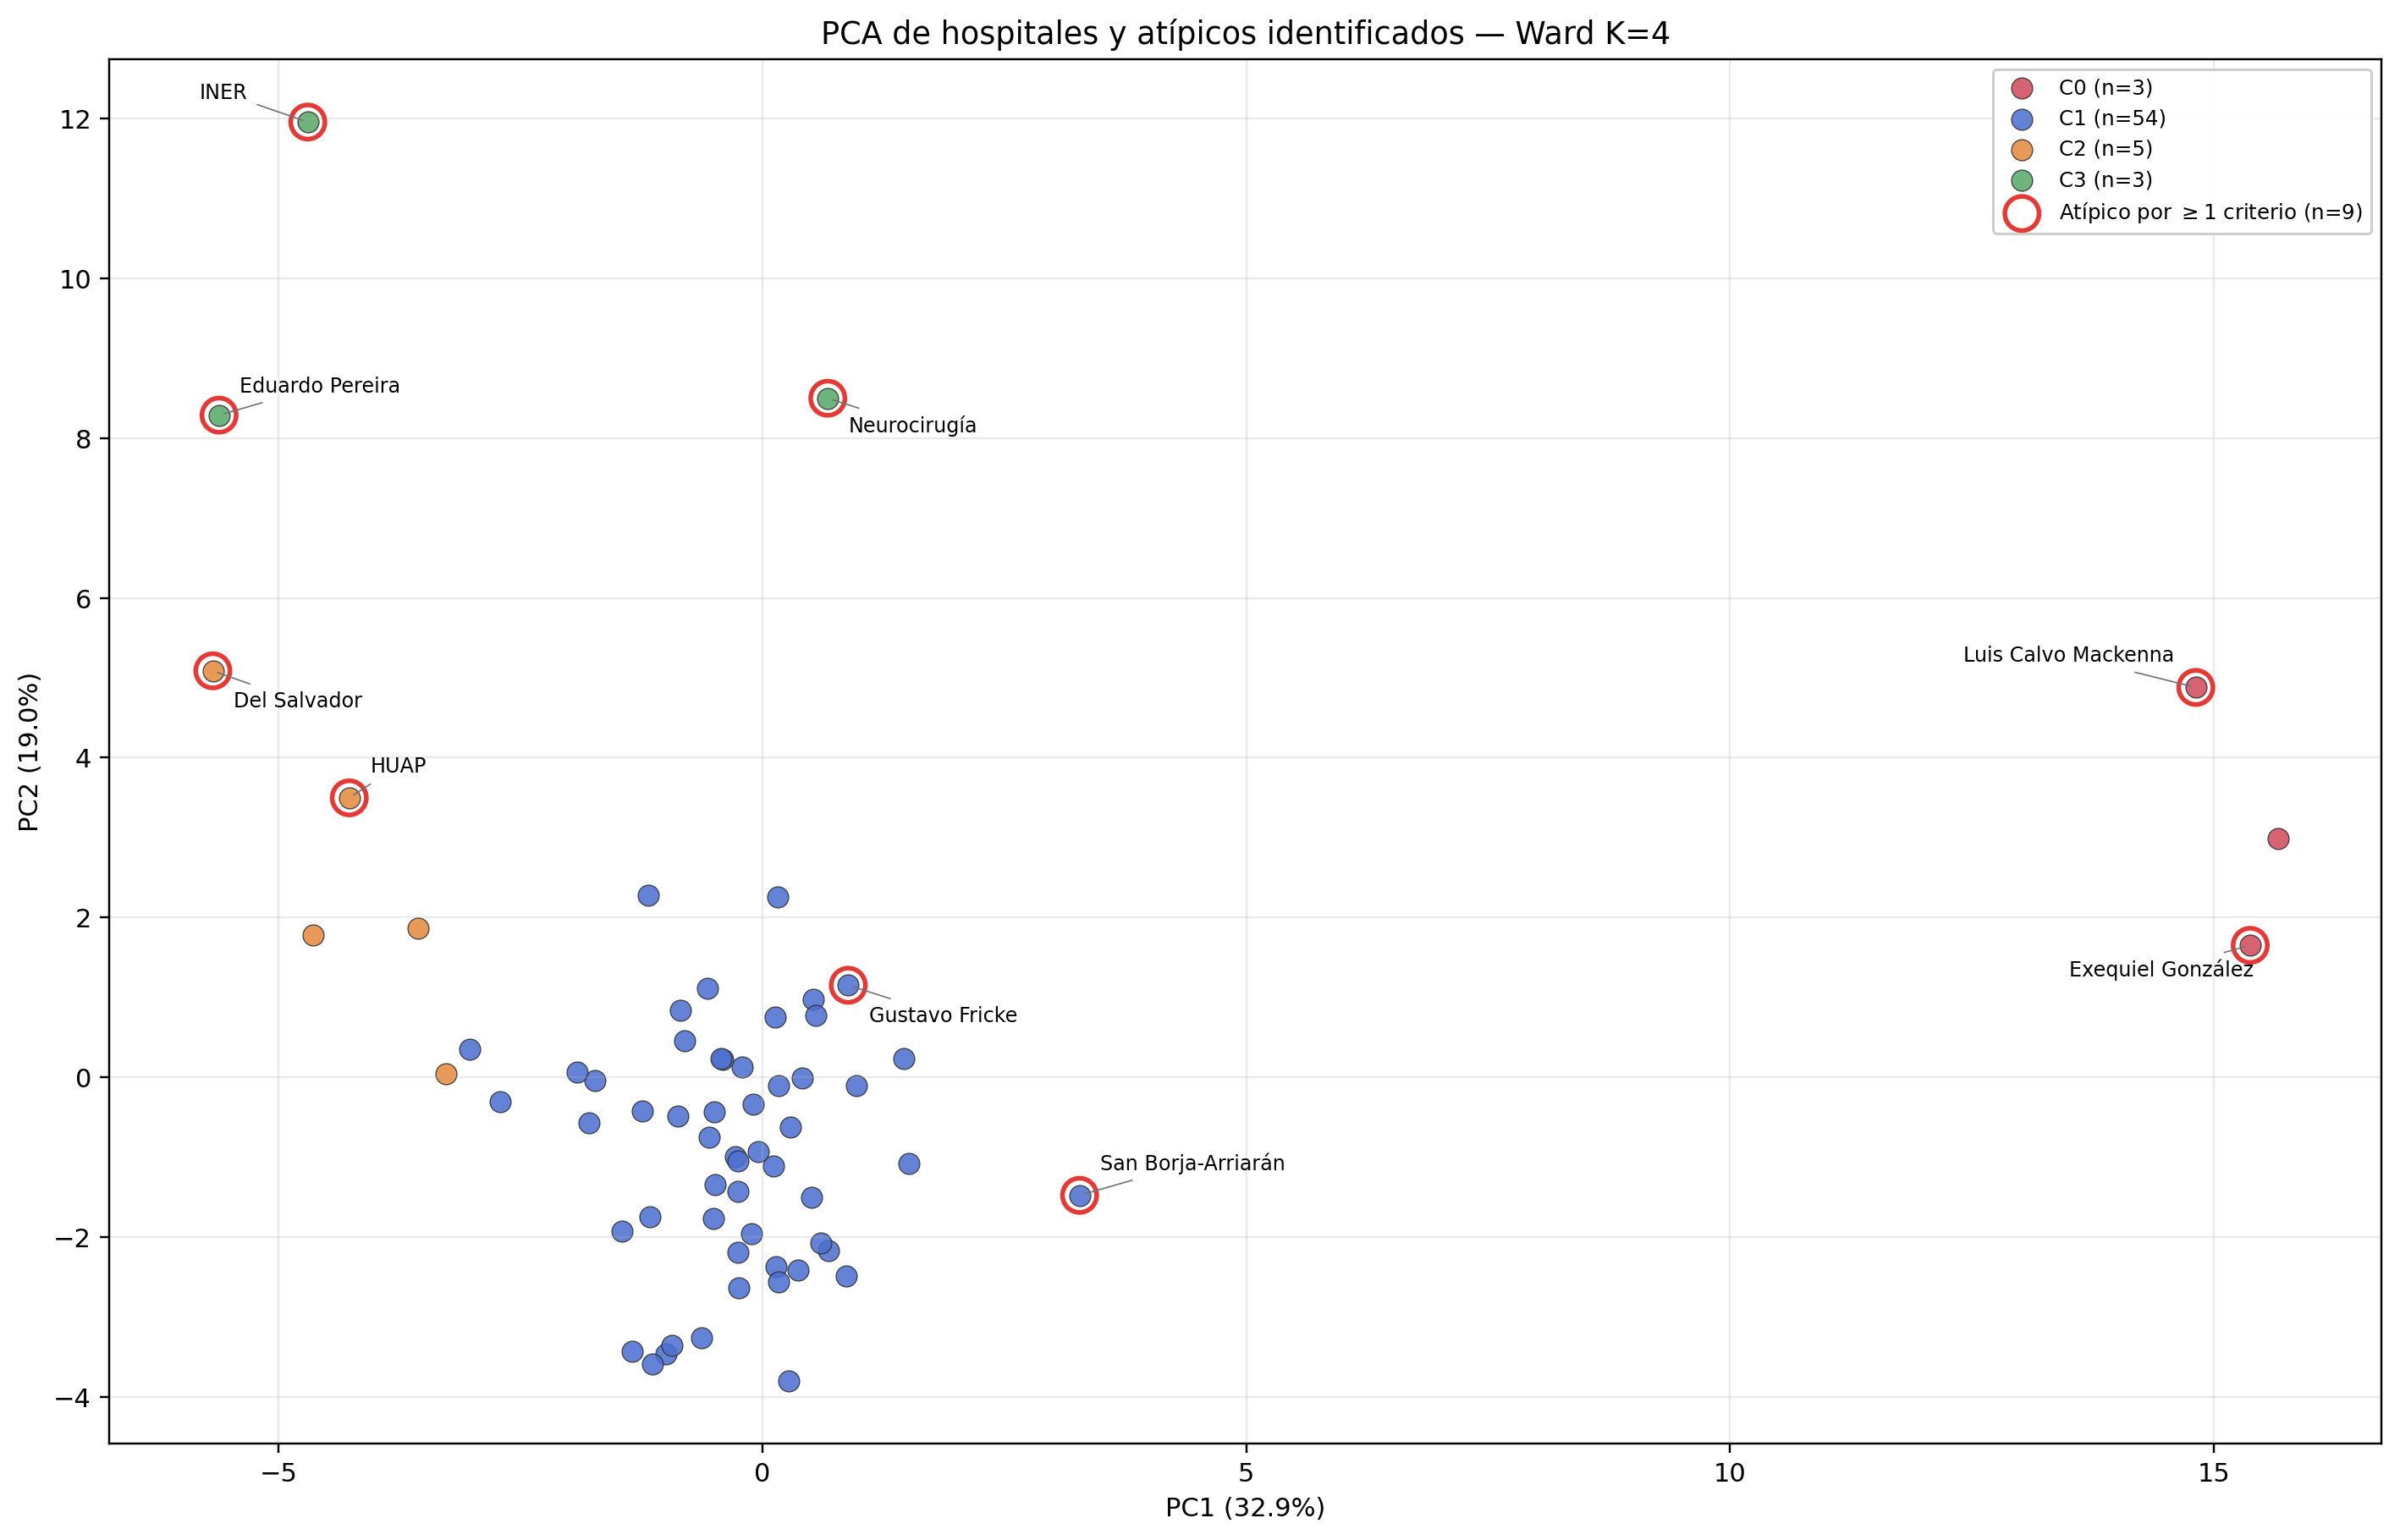
\includegraphics[width=\textwidth]{img/atipicos_pca.png}
\caption{Proyección PCA de los establecimientos, partición Ward $K=4$. Los círculos rojos indican hospitales atípicos.}
\label{fig:outliers-pca}
\end{figure}


\section{Sensibilidad algorítmica, temporal y composicional}

\label{sec:sensibilidad-analisis}

Antes de presentar los resultados, es necesario delimitar el alcance de estas comparaciones. Los algoritmos alternativos, las proyecciones bidimensionales y la solución Ward principal se construyen sobre la misma matriz de 35 variables y el mismo conjunto de 65 hospitales. Por ello, las comparaciones algorítmicas corresponden a un análisis de sensibilidad interna y no a una validación externa. Una validación externa requeriría contrastar la partición con hospitales, períodos o fuentes de información no utilizados en su construcción, lo que no se dispone en este estudio.

La proyección PCA presentada en la Sección~\ref{sec:res-outliers} tiene un propósito exploratorio y descriptivo. Permite observar una representación bidimensional de las mismas etiquetas Ward, pero no constituye un algoritmo alternativo de clustering ni evidencia independiente de la estabilidad de la partición. Por esta razón, la sensibilidad algorítmica se evalúa mediante MST-kNN, K-means y mezclas gaussianas, junto con índices cuantitativos de concordancia entre particiones.

\subsection*{Sensibilidad frente al algoritmo MST-kNN}

Se aplicó el algoritmo MST-kNN~\citep{inostroza2008} sobre la misma matriz institucional utilizada por Ward, explorando valores de $k$ entre 3 y 8 en modo mutuo. En esta configuración, dos hospitales se consideran vecinos solo cuando la relación de vecindad es recíproca. El algoritmo no impone un número fijo de grupos y puede producir grupos unitarios o pares, por lo que sus resultados no son directamente equivalentes a una partición de cuatro clústeres.

La Tabla~\ref{tab:mstknn-sensibilidad} presenta el comportamiento de la solución al variar $k$. A medida que aumenta el número de vecinos, disminuyen los grupos descubiertos y los grupos unitarios, mientras que el bloque de mayor tamaño aumenta desde 23 hospitales con $k=3$ hasta 38 con $k=8$. Esto muestra que la granularidad obtenida mediante MST-kNN depende de la definición de vecindad seleccionada.

\begin{table}[htbp]
\centering
\caption{Resultados del análisis de sensibilidad con MST-kNN en modo mutuo.}
\label{tab:mstknn-sensibilidad}

\begin{tabular}{c c c c c l}
\toprule
\textbf{$k$} & \textbf{$K$ total} & \textbf{Grupos $n\geq3$} & \textbf{Pares} & \textbf{Unitarios} & \textbf{Tamaños de grupos $n\geq3$} \\
\midrule
3 & 26 & 5 & 6 & 15 & [23, 5, 4, 3, 3] \\
4 & 25 & 5 & 6 & 14 & [23, 5, 5, 3, 3] \\
5 & 22 & 5 & 7 & 10 & [25, 5, 5, 3, 3] \\
6 & 21 & 5 & 6 & 10 & [27, 5, 5, 3, 3] \\
7 & 17 & 5 & 5 & 7 & [34, 5, 3, 3, 3] \\
8 & 14 & 5 & 4 & 5 & [38, 5, 3, 3, 3] \\
\bottomrule
\end{tabular}
\end{table}

Entre las configuraciones exploradas, $k=8$ alcanza el mayor Silhouette interno ($0{,}075$), aunque mantiene 14 grupos, incluidos cinco grupos unitarios. Por otro lado, $k=6$ genera 21 grupos, cinco de ellos con al menos tres hospitales, seis pares y diez grupos unitarios. Ninguna de estas configuraciones reproduce una partición compacta de cuatro grupos comparable directamente con Ward. En consecuencia, MST-kNN se interpreta como una sensibilidad a una definición local de vecindad y no como un método destinado a seleccionar una solución alternativa única.

El resultado principal del barrido es que el núcleo generalista no permanece como un bloque único al exigir vecindades mutuas locales. Dependiendo de $k$, este núcleo se divide en un grupo principal, grupos pequeños y hospitales unitarios. Esta diferencia es consistente con la naturaleza del método, que prioriza conexiones locales recíprocas y no minimiza la varianza intragrupo bajo el mismo criterio que Ward.

\subsection*{Concordancia cuantitativa entre particiones alternativas}

Para cuantificar la sensibilidad algorítmica, se calcularon el Índice de Rand Ajustado (ARI) y la Información Mutua Normalizada (NMI) entre la solución Ward $K=4$ y tres algoritmos alternativos construidos sobre la misma matriz: K-means con $K=4$, GMM con $K=4$ y MST-kNN con $k=6$ en modo mutuo. Además, se comparó el bloque generalista más grande mediante el índice de Jaccard y su recall respecto del núcleo generalista de Ward. Para los hospitales especializados, se calculó la proporción que permanece fuera del bloque principal de cada algoritmo alternativo. Los resultados se presentan en la Tabla~\ref{tab:concordancia-sensibilidad}.

\begin{table}[htbp]
\centering
\caption{Concordancia cuantitativa entre la partición Ward $K=4$ y particiones alternativas.}
\label{tab:concordancia-sensibilidad}
\resizebox{\textwidth}{!}{%
\begin{tabular}{l c c c c c}
\toprule
\textbf{Partición alternativa} &
\textbf{ARI} &
\textbf{NMI} &
\textbf{Jaccard núcleo} &
\textbf{Recall núcleo} &
\textbf{Recall especializados fuera del núcleo} \\
\midrule
K-means ($K=4$) &
0,927 &
0,851 &
0,982 &
0,982 &
1,000 \\

GMM ($K=4$) &
0,314 &
0,520 &
0,546 &
0,556 &
0,909 \\

MST-kNN ($k=6$, mutuo) &
0,180 &
0,429 &
0,500 &
0,500 &
1,000 \\
\bottomrule
\end{tabular}%
}
\end{table}

K-means presenta una concordancia alta con Ward, con $\text{ARI}=0{,}927$ y $\text{NMI}=0{,}851$. El bloque principal de K-means contiene 53 de los 54 hospitales del núcleo generalista Ward, y todos los hospitales especializados permanecen fuera de dicho bloque. Esta coincidencia es informativa, aunque debe interpretarse considerando que K-means y Ward comparten una preferencia por grupos compactos bajo distancia euclidiana. Por tanto, no constituyen mecanismos completamente independientes.

GMM y MST-kNN muestran una concordancia menor con la partición completa. Para GMM, el ARI es $0{,}314$ y el NMI es $0{,}520$; para MST-kNN, el ARI es $0{,}180$ y el NMI es $0{,}429$. Estos resultados indican que ambos algoritmos reorganizan una parte relevante de la partición Ward, especialmente dentro del núcleo generalista. En efecto, el recall del núcleo generalista es $0{,}556$ para GMM y $0{,}500$ para MST-kNN.

La separación entre el núcleo generalista y los hospitales especializados presenta una persistencia mayor que la composición interna del núcleo. MST-kNN mantiene a todos los hospitales especializados fuera de su bloque principal, mientras que GMM mantiene fuera a $90{,}9\%$ de ellos. Esta evidencia no implica que los grupos especializados se reproduzcan de manera idéntica entre métodos, sino que su diferenciación respecto del bloque generalista tiende a conservarse mejor que las fronteras internas del núcleo.

En conjunto, los resultados describen una sensibilidad algorítmica asimétrica. La distinción entre hospitales especializados y el núcleo generalista se mantiene en mayor medida bajo mecanismos alternativos, mientras que la asignación detallada de los hospitales que integran el núcleo generalista depende más del algoritmo utilizado.

\subsection*{Sensibilidad temporal: exclusión de los años de pandemia (2020--2021)}

Siguiendo el procedimiento descrito en la Sección~\ref{sec:sensibilidad-temporal}, se reconstruyó la matriz institucional excluyendo los años 2020 y 2021, manteniendo el mismo universo de 65 hospitales. Posteriormente, se aplicó nuevamente Ward con $K=4$ y se comparó la partición obtenida con la solución construida sobre el período completo 2019--2024.

La solución sin pandemia presenta un Silhouette de $0{,}356$ y tamaños de grupo $[3,51,2,9]$, frente al Silhouette de $0{,}400$ y los tamaños $[3,54,5,3]$ de la partición principal. La concordancia entre ambas soluciones alcanza $\text{ARI}=0{,}809$ y $\text{NMI}=0{,}750$, lo que indica una estabilidad importante, aunque no completa. La distribución de las reasignaciones se detalla en la Tabla~\ref{tab:contingencia-temporal}.

\begin{table}[htbp]
\centering
\caption{Contingencia entre la partición Ward $K=4$ (período completo) y la solución sin 2020--2021.}
\label{tab:contingencia-temporal}
\begin{tabular}{c c c c c}
\toprule
\textbf{Original $\backslash$ Sin pandemia} & \textbf{0} & \textbf{1} & \textbf{2} & \textbf{3} \\
\midrule
\textbf{0} ($C0$) & 3 & 0 & 0 & 0 \\
\textbf{1} ($C1$) & 0 & 51 & 0 & 3 \\
\textbf{2} ($C2$) & 0 & 0 & 0 & 5 \\
\textbf{3} ($C3$) & 0 & 0 & 2 & 1 \\
\bottomrule
\end{tabular}
\end{table}

Los tres hospitales de $C0$ permanecen agrupados al excluir los años de pandemia. En el núcleo generalista, 51 de los 54 hospitales permanecen en el bloque principal de la solución temporal alternativa, mientras que tres se reasignan a otro grupo. Los cambios restantes se concentran en los grupos pequeños $C2$ y $C3$. Por tanto, la estructura global se conserva en términos generales, pero los límites entre los perfiles de menor tamaño son más sensibles a la ventana temporal considerada.

La sensibilidad temporal por variable se concentra especialmente en algunas componentes de casuística. Las componentes \texttt{dim\_07} y \texttt{dim\_08} presentan cambios relativos medianos de $124{,}7\%$ y $104{,}7\%$, respectivamente, mientras que \texttt{tasa\_partos} presenta un cambio relativo mediano de $41{,}0\%$. Estos resultados indican que las interpretaciones clínicas finas asociadas a componentes específicas del PCA son más sensibles a la exclusión de 2020--2021 que los perfiles funcionales globales.

Como contraste adicional, se ponderaron las ocho componentes por la raíz de su
varianza explicada: \texttt{dim\_01} explica $22{,}8\%$ y \texttt{dim\_08}
$3{,}4\%$. La ponderación mejoró las métricas internas (Silhouette de $0{,}401$
a $0{,}446$; Davies--Bouldin de $0{,}990$ a $0{,}881$), pero reorganizó tres
hospitales entre los dos grupos pequeños ($ARI=0{,}992$; $NMI=0{,}944$). Por
ello se mantiene la ponderación uniforme de la solución canónica y el resultado
ponderado se interpreta como evidencia de sensibilidad: la estructura global
persiste, pero las fronteras finas entre perfiles especializados dependen del
peso asignado a la casuística.

Los 65 hospitales del universo final poseen cobertura completa para los seis años del período analizado. En consecuencia, no se compararon hospitales con cobertura temporal completa e incompleta dentro de esta muestra, ya que dicha heterogeneidad fue removida previamente por el criterio de elegibilidad descrito en la Sección~\ref{sec:elegibilidad}.

\subsection*{Sensibilidad composicional: transformación CLR de la casuística}

Siguiendo el procedimiento descrito en la Sección~\ref{sec:sensibilidad-composicional}, se reconstruyó la representación de casuística aplicando una transformación CLR a los vectores composicionales antes del PCA. Esta alternativa considera explícitamente que las proporciones de capítulos diagnósticos, procedimientos y GRD forman composiciones sujetas a la restricción de suma constante.

La partición obtenida mediante CLR+PCA reproduce exactamente la asignación Ward principal: $\text{ARI}=1{,}000$, $\text{NMI}=1{,}000$ y cero hospitales cambian de clúster. Los tamaños de los grupos se mantienen en $[3,54,5,3]$, como confirma la Tabla~\ref{tab:contingencia-clr}.

\begin{table}[htbp]
\centering
\caption{Contingencia entre la partición Ward con PCA convencional y con CLR+PCA.}
\label{tab:contingencia-clr}
\begin{tabular}{c c c c c}
\toprule
\textbf{PCA convencional $\backslash$ CLR+PCA} & \textbf{0} & \textbf{1} & \textbf{2} & \textbf{3} \\
\midrule
\textbf{0} ($C0$) & 3 & 0 & 0 & 0 \\
\textbf{1} ($C1$) & 0 & 54 & 0 & 0 \\
\textbf{2} ($C2$) & 0 & 0 & 5 & 0 \\
\textbf{3} ($C3$) & 0 & 0 & 0 & 3 \\
\bottomrule
\end{tabular}
\end{table}

La solución CLR+PCA presenta un Silhouette de $0{,}438$, frente a $0{,}400$ con la representación convencional. Además, las ocho componentes principales explican $76{,}9\%$ de la varianza en la representación CLR, frente a $72{,}3\%$ con PCA convencional. Estas diferencias muestran que la transformación CLR mejora la representación de la casuística bajo estos indicadores, pero no modifica la identidad de los cuatro perfiles obtenidos.

Por tanto, la posible clausura de las proporciones no altera la partición principal en este conjunto de datos. Este resultado respalda la estabilidad de los perfiles funcionales frente a una alternativa composicionalmente adecuada, aunque no convierte la solución en una validación externa.

\subsection*{Sensibilidad al criterio de elegibilidad de hospitales}

Como análisis adicional, se eliminó el requisito de cobertura temporal completa y se reconstruyó la matriz sobre 72 hospitales. Al restringir la comparación a los 65 hospitales compartidos con el análisis principal, la concordancia alcanza $\text{ARI}=0{,}936$ y $\text{NMI}=0{,}909$. La solución ampliada presenta tamaños $[3,53,12,4]$ y un Silhouette de $0{,}347$.

La disminución de cohesión respecto de la solución principal ($0{,}400$) y la concentración de seis de los siete hospitales con cobertura parcial en un mismo grupo sugieren que la inclusión de establecimientos con series temporales incompletas introduce perfiles institucionales menos comparables con el resto de la muestra. El criterio de elegibilidad se mantiene, por tanto, como una decisión para asegurar comparabilidad temporal, sin atribuirle la creación artificial de la estructura principal.

\subsection*{Síntesis de los análisis de sensibilidad}

Los resultados de sensibilidad muestran patrones diferenciados según el tipo de perturbación aplicada. La transformación CLR conserva exactamente la partición principal, mientras que la exclusión de 2020--2021 reduce la concordancia a $\text{ARI}=0{,}809$ y reorganiza principalmente los grupos de menor tamaño. La ampliación del universo a 72 hospitales mantiene una concordancia alta con la solución principal, aunque reduce la cohesión interna y concentra los establecimientos con cobertura incompleta.

Frente al cambio de algoritmo, la evidencia es asimétrica. K-means presenta una concordancia elevada con Ward, mientras que GMM y MST-kNN reorganizan de forma más importante la partición completa. Sin embargo, ambos métodos tienden a conservar, en distinta magnitud, la separación entre el bloque generalista y los establecimientos especializados. En consecuencia, los perfiles especializados muestran mayor persistencia frente a cambios metodológicos que la composición detallada del núcleo generalista.

Finalmente, la sensibilidad temporal afecta especialmente algunas componentes de casuística y la proporción de egresos neonatales. Por ello, la interpretación de los perfiles funcionales globales cuenta con mayor respaldo que una lectura exhaustiva de las componentes específicas del PCA o de diferencias clínicas finas entre los grupos.

% ============================================================================
%  CAPÍTULO 5 — CONCLUSIONES
% ============================================================================

\chapter{Conclusiones}
\label{cap:conclusiones}

Esta investigación caracterizó funcionalmente a los hospitales públicos chilenos
de alta y mediana complejidad a partir de registros administrativos GRD del
período 2019--2024. El pipeline reproducible construido transforma los egresos
registrados con fines administrativos en una representación institucional basada
en producción, complejidad, diversidad, casuística, modalidad de ingreso y alta,
composición demográfica y actividad quirúrgico-obstétrica.

La respuesta a la pregunta de investigación es afirmativa: los datos GRD permiten
identificar perfiles funcionales distinguibles que no coinciden de forma estrecha
con la clasificación administrativa vigente. La solución Ward con $K=4$, aplicada
sobre una matriz de $65 \times 35$ variables, distingue tres hospitales
pediátricos, un núcleo generalista de 54 establecimientos, un grupo de cinco
hospitales con carga clínica y estancia prolongada, y tres institutos
monográficos. La elección de cuatro grupos se sostiene como un compromiso
interpretativo: la solución $K=2$ maximiza las métricas internas, pero reduce la
red a un bloque de 62 hospitales y tres casos singulares, lo que no permite el
perfilamiento funcional propuesto.

La matriz final integra 27 variables clínico-operativas directas y ocho
componentes principales de casuística. Estas componentes condensan
aproximadamente el $72{,}3\,\%$ de la varianza de las proporciones construidas a
partir de capítulos CIE-10, secciones CIE-9-MC y GRD frecuentes. La cobertura
ampliada de los campos diagnósticos y de procedimientos permite incorporar una
parte sustantiva de la información clínica registrada. Sin embargo, indicadores
como las comorbilidades promedio deben interpretarse como carga clínica
registrada, pues pueden reflejar simultáneamente diferencias de casuística y
diferencias en la exhaustividad de la codificación entre establecimientos.

La comparación con MINSAL confirma que las dos clasificaciones describen
dimensiones diferentes de la red. La concordancia entre Ward $K=4$ y las
categorías de Alta y Mediana Complejidad fue baja
(ARI $=0{,}112$; NMI $=0{,}107$). En particular, el núcleo generalista contiene
47 hospitales de Alta y 7 de Mediana Complejidad, mientras que el grupo de carga
clínica reúne 2 y 3 establecimientos, respectivamente. Esta divergencia no
implica que una clasificación sea intrínsecamente correcta y la otra incorrecta;
indica que la clasificación administrativa y el patrón de producción clínica no
son intercambiables.

La hipótesis de mayor homogeneidad funcional se evaluó directamente sobre la
misma matriz preprocesada. Ward $K=4$ obtuvo una dispersión intragrupo
normalizada WSS/TSS $=0{,}475$ y Silhouette $=0{,}401$, frente a WSS/TSS
$=0{,}944$ y Silhouette $=0{,}070$ para MINSAL. Al controlar el número de
grupos, Ward $K=2$ mantuvo menor dispersión que MINSAL
(WSS/TSS $=0{,}707$ frente a $0{,}944$). Las pruebas de permutación con 2.000
reasignaciones preservando los tamaños de grupo confirman que ambas particiones
son más homogéneas que asignaciones aleatorias comparables, aunque la distancia
respecto de la distribución nula es considerablemente mayor para las soluciones
Ward. Por tanto, la evidencia respalda que la segmentación funcional produce
grupos más homogéneos en el espacio de variables utilizado, sin que ello
constituya una validación externa de su utilidad operativa.

Los análisis de estabilidad y sensibilidad matizan el alcance de esta conclusión.
En 100 submuestras sin reposición del $80\,\%$ de los hospitales, la mediana del
ARI respecto de la solución completa fue $0{,}958$ y la del NMI fue $0{,}917$.
La transformación composicional CLR conservó exactamente la partición principal
(ARI $=1{,}000$), con un Silhouette de $0{,}438$. En cambio, la exclusión de los
años 2020--2021 produjo una concordancia menor
(ARI $=0{,}809$; NMI $=0{,}750$). En consecuencia, la separación global de los
perfiles se sostiene bajo estas perturbaciones, pero las fronteras entre grupos
pequeños y la interpretación de componentes finas de casuística son sensibles al
período y a la representación utilizada.

El análisis descriptivo posterior al agrupamiento, realizado variable por variable,
identificó diferencias significativas, tras la corrección de
Benjamini--Hochberg, en 26 de las 28 variables directas entre los cuatro grupos
de Nivel 1. Este resultado permite caracterizar los perfiles obtenidos, pero no
constituye una prueba independiente de la partición, porque las mismas variables
participaron en su construcción. La prueba de permutación del flujo completo
acota esta circularidad: ninguna de las 500 matrices sin estructura real alcanzó
las 26 variables significativas observadas. Aun así, esta evidencia no reemplaza
una validación externa con nuevos años, hospitales o variables no utilizadas para
descubrir la partición.

La interpretación de los grupos debe mantener una distinción fundamental: los
perfiles identificados describen actividad clínica registrada, pero no miden
calidad, desempeño ni eficiencia. El estudio no incorporó costos, camas,
equipamiento, dotación de personal, tiempos de espera ni desenlaces posteriores
al alta. Por ello, los resultados pueden apoyar una caracterización
complementaria de la red, pero no justifican por sí solos decisiones de
financiamiento, asignación de recursos o evaluación de desempeño institucional.

Las principales limitaciones se relacionan con la naturaleza administrativa de
los datos, la heterogeneidad en las prácticas de codificación, la inclusión de
los años afectados por la pandemia de COVID-19, la geometría composicional de
los vectores de casuística y la ausencia de validación externa independiente.
La prueba CLR indica que la clausura composicional no alteró la identidad de los
cuatro grupos en este análisis, pero no excluye que otras transformaciones, como
ILR, aporten matices adicionales. Del mismo modo, la estabilidad temporal permite
sostener la existencia de perfiles generales, pero no interpretar de manera
rígida las asignaciones que se encuentran próximas a los límites entre grupos.

Como trabajo futuro, resulta prioritario validar longitudinalmente el pipeline
con nuevos años de egresos y evaluar su generalización al incorporar hospitales
recientemente integrados al sistema GRD. También sería relevante combinar el
perfil funcional con demanda territorial, recursos humanos, camas, costos y
resultados clínicos. Esa integración permitiría pasar desde una tipología
descriptiva de la producción hacia análisis más completos de organización,
capacidad y eficiencia de la red asistencial.


{\setstretch{1.0}                           % Interlineado páginas finales
% ### Glosario (optativo; no utilizado) ###
%\clearpage
%\addcontentsline{toc}{chapter}{Glosario}
%\input{finales/Glosario}

% ### Bibliografía de la tesis ###
\clearpage
\phantomsection
\addcontentsline{toc}{chapter}{Referencias bibliogr\'aficas}
\bibliographystyle{apa-good}
\bibliography{bibliografia}

% ### Anexos de la tesis ###
\clearpage
\phantomsection
\anexo
\addcontentsline{toc}{chapter}{Anexos}
% ============================================================================
%  ANEXO A — MATERIAL COMPLEMENTARIO
% ============================================================================

\chapter{Material complementario}
\label{anexo:complementario}

Este anexo reúne antecedentes de respaldo para la caracterización funcional
presentada en los Capítulos~\ref{cap:metodologia} y~\ref{cap:resultados}. Se
incluyen el diccionario de variables institucionales, el listado de
establecimientos incluidos y excluidos, la asignación final de clústeres y los
principales parámetros del pipeline computacional.

\section{Diccionario de variables institucionales}
\label{anexo:diccionario}

La Tabla~\ref{tab:anexo-diccionario} detalla las 28 variables
clínico-operativas directas construidas a nivel institucional. La variable
\texttt{peso\_medio\_cma} se conserva para fines descriptivos, pero fue excluida
de la matriz empleada en el clustering debido a que no es estructuralmente
comparable entre todos los establecimientos. Las 27 variables directas restantes,
junto con las 8 componentes principales de casuística
(\texttt{dim\_01} a \texttt{dim\_08}), conforman la matriz final de
$65 \times 35$ variables descrita en la Sección~\ref{sec:matriz-final}.

\begin{longtable}{p{4.0cm} p{5.8cm} p{2.0cm} p{2.2cm}}
\caption{Diccionario de las 28 variables clínico-operativas directas construidas a nivel institucional.}
\label{tab:anexo-diccionario} \\
\toprule
\textbf{Variable} & \textbf{Definición operacional} & \textbf{Unidad} & \textbf{Grupo} \\
\midrule
\endfirsthead

\multicolumn{4}{c}{\tablename\ \thetable{} -- continuación} \\
\toprule
\textbf{Variable} & \textbf{Definición operacional} & \textbf{Unidad} & \textbf{Grupo} \\
\midrule
\endhead

\texttt{egresos\_por\_anio} &
Promedio anual de egresos de hospitalización convencional durante el período analizado. &
Conteo & Actividad \\

\texttt{estancia\_media} &
Media aritmética de los días de estancia entre ingreso y alta. &
Días & Estadía \\

\texttt{estancia\_mediana} &
Mediana de los días de estancia entre ingreso y alta. &
Días & Estadía \\

\texttt{peso\_medio\_grd} &
Promedio del peso relativo GRD de los egresos del establecimiento. &
Adimensional & Complejidad \\

\texttt{severidad\_media} &
Promedio del índice de severidad clínica asignado por el agrupador GRD. &
Adimensional (1--4) & Complejidad \\

\texttt{mortalidad\_media} &
Promedio del índice de riesgo de mortalidad asignado por el agrupador GRD. &
Adimensional (1--4) & Complejidad \\

\texttt{entropia\_grd} &
Entropía de Shannon de la distribución de GRD del establecimiento. &
Bits & Diversidad \\

\texttt{comorbilidades\_promedio} &
Promedio de diagnósticos secundarios registrados por egreso. &
Conteo & Diversidad \\

\texttt{tasa\_cma} &
Proporción de egresos registrados como Cirugía Mayor Ambulatoria sobre el total institucional. &
Proporción & CMA \\

\texttt{peso\_medio\_cma} &
Promedio del peso relativo GRD entre los egresos de CMA. Se emplea de forma descriptiva y se excluye del clustering final. &
Adimensional & CMA \\

\texttt{pct\_pediatrico} &
Proporción de egresos de pacientes menores de 15 años. &
Proporción & Perfil demográfico \\

\texttt{pct\_geriatrico} &
Proporción de egresos de pacientes de 65 años o más. &
Proporción & Perfil demográfico \\

\texttt{pct\_femenino\_fertil} &
Proporción de egresos de mujeres entre 15 y 49 años. &
Proporción & Perfil demográfico \\

\texttt{edad\_mediana} &
Mediana de edad al ingreso de los egresos institucionales. &
Años & Perfil demográfico \\

\texttt{pct\_urgencia} &
Proporción de egresos cuyo tipo de ingreso fue urgencia. &
Proporción & Modalidad de ingreso \\

\texttt{pct\_programada} &
Proporción de egresos cuyo tipo de ingreso fue programado. &
Proporción & Modalidad de ingreso \\

\texttt{pct\_obstetrica\_ingreso} &
Proporción de egresos cuyo tipo de ingreso fue obstétrico. &
Proporción & Modalidad de ingreso \\

\texttt{pct\_alta\_domicilio} &
Proporción de egresos con alta a domicilio. &
Proporción & Tipo de alta \\

\texttt{pct\_alta\_fallecido} &
Proporción de egresos con alta por defunción. &
Proporción & Tipo de alta \\

\texttt{pct\_alta\_traslado} &
Proporción de egresos con alta por traslado o derivación a otro establecimiento. &
Proporción & Tipo de alta \\

\texttt{pct\_origen\_emergencia} &
Proporción de egresos procedentes del servicio de urgencia propio. &
Proporción & Procedencia \\

\texttt{pct\_origen\_referencia} &
Proporción de egresos derivados desde otro establecimiento de la red. &
Proporción & Procedencia \\

\texttt{pct\_uso\_pabellon} &
Proporción de egresos con al menos un uso de pabellón quirúrgico registrado. &
Proporción & Actividad quirúrgica \\

\texttt{pabellones\_promedio} &
Promedio de usos de pabellón por egreso hospitalizado. &
Conteo & Actividad quirúrgica \\

\texttt{tasa\_partos} (nombre técnico legado) &
Proporción de egresos hospitalarios con condición de alta neonatal registrada; no equivale a una tasa ni a un conteo de partos atendidos. &
Proporción & Actividad neonatal \\

\texttt{tasa\_prematurez} &
Proporción de egresos neonatales registrados con peso de nacimiento inferior a 2.500 gramos. &
Proporción & Actividad neonatal \\

\texttt{pct\_estancia\_larga} &
Proporción de egresos con estancia superior a 30 días. &
Proporción & Estadía \\

\texttt{cv\_estancia} &
Coeficiente de variación de la duración de estancia. &
Adimensional & Estadía \\

\bottomrule
\end{longtable}

Las ocho componentes de casuística
(\texttt{dim\_01}--\texttt{dim\_08}) se obtuvieron mediante PCA de la matriz
de proporciones diagnósticas, de procedimientos y de GRD descrita en la
Sección~\ref{sec:pca-detalle}. Cada componente es una combinación lineal de las
variables originales, por lo que no posee una definición operacional única. Su
interpretación se realiza mediante las cargas de mayor magnitud y debe
considerarse complementaria a las variables institucionales directas.

\section{Establecimientos incluidos, excluidos y asignación final}
\label{anexo:hospitales}

De los 72 establecimientos con datos GRD disponibles durante 2019--2024, 65
cumplieron el criterio de presencia temporal mínima de tres de los seis años del
período y conformaron el universo final de análisis. Los siete establecimientos
excluidos se presentan en la Tabla~\ref{tab:anexo-excluidos}.

\begin{table}[htbp]
\centering
\caption{Establecimientos excluidos por no cumplir el criterio de presencia temporal mínima.}
\label{tab:anexo-excluidos}
\begin{tabular}{c c}
\toprule
\textbf{Código} & \textbf{Años con presencia válida} \\
\midrule
110110 & 2 \\
116107 & 1 \\
116111 & 1 \\
118106 & 2 \\
119101 & 2 \\
119102 & 1 \\
200717 & 1 \\
\bottomrule
\end{tabular}
\end{table}

La partición final de Nivel~1 contiene tres hospitales pediátricos ($C0$), un
núcleo generalista de 54 establecimientos ($C1$), un grupo de cinco hospitales
con carga clínica y estancia prolongada ($C2$), y tres institutos monográficos
($C3$). El núcleo generalista se subdividió de forma exploratoria mediante
Ward con $K_{sub}=10$, cuyas etiquetas se presentan como $S0$ a $S9$.

La Tabla~\ref{tab:anexo-hospitales} presenta la asignación final de los 65
establecimientos. Las etiquetas de Nivel~2 solo se aplican a los miembros de
$C1$; no constituyen categorías funcionales validadas equivalentes a los grupos
del Nivel~1.

\begin{longtable}{p{1.5cm} p{9.0cm} p{1.0cm} p{1.0cm}}
\caption{Asignación final de los establecimientos en los Niveles 1 y 2 del clustering Ward.}
\label{tab:anexo-hospitales} \\
\toprule
\textbf{Código} & \textbf{Establecimiento} & \textbf{N1} & \textbf{N2} \\
\midrule
\endfirsthead

\multicolumn{4}{c}{\tablename\ \thetable{} -- continuación} \\
\toprule
\textbf{Código} & \textbf{Establecimiento} & \textbf{N1} & \textbf{N2} \\
\midrule
\endhead

101100 & Hospital Dr.\ Juan Noé Crevanni (Arica) & $C1$ & $S6$ \\
102100 & Hospital Dr.\ Ernesto Torres Galdames (Iquique) & $C1$ & $S6$ \\
103100 & Hospital Dr.\ Leonardo Guzmán (Antofagasta) & $C1$ & $S8$ \\
103101 & Hospital Dr.\ Carlos Cisternas (Calama) & $C1$ & $S6$ \\
104100 & Hospital San José del Carmen (Copiapó) & $C1$ & $S6$ \\
104103 & Hospital Provincial del Huasco Monseñor Fernando Ariztía Ruiz (Vallenar) & $C1$ & $S6$ \\
105100 & Hospital San Juan de Dios (La Serena) & $C1$ & $S5$ \\
105101 & Hospital San Pablo (Coquimbo) & $C1$ & $S6$ \\
105102 & Hospital Dr.\ Antonio Tirado Lanas (Ovalle) & $C1$ & $S5$ \\
106100 & Hospital Carlos Van Buren (Valparaíso) & $C1$ & $S8$ \\
106102 & Hospital Dr.\ Eduardo Pereira Ramírez (Valparaíso) & $C3$ & --- \\
106103 & Hospital Claudio Vicuña (San Antonio) & $C1$ & $S0$ \\
107100 & Hospital Dr.\ Gustavo Fricke (Viña del Mar) & $C1$ & $S9$ \\
107101 & Hospital San Martín (Quillota) & $C1$ & $S5$ \\
107102 & Hospital de Quilpué & $C1$ & $S1$ \\
108100 & Hospital de San Camilo (San Felipe) & $C1$ & $S5$ \\
108101 & Hospital San Juan de Dios (Los Andes) & $C1$ & $S6$ \\
109100 & Complejo Hospitalario San José (Santiago, Independencia) & $C1$ & $S3$ \\
109101 & Hospital Clínico de Niños Dr.\ Roberto del Río & $C0$ & --- \\
110100 & Hospital San Juan de Dios (Santiago) & $C1$ & $S8$ \\
110120 & Hospital Dr.\ Félix Bulnes Cerda & $C1$ & $S3$ \\
110130 & Hospital Adalberto Steeger (Talagante) & $C1$ & $S2$ \\
110150 & Hospital San José (Melipilla) & $C1$ & $S2$ \\
111100 & Hospital Clínico San Borja-Arriarán & $C1$ & $S4$ \\
111101 & Hospital Clínico Metropolitano El Carmen Dr.\ Luis Valentín Ferrada & $C1$ & $S7$ \\
111195 & Hospital de Urgencia Asistencia Pública Dr.\ Alejandro del Río & $C2$ & --- \\
112100 & Hospital Del Salvador (Santiago, Providencia) & $C2$ & --- \\
112101 & Hospital Dr.\ Luis Tisné B. & $C1$ & $S3$ \\
112102 & Hospital de Niños Dr.\ Luis Calvo Mackenna & $C0$ & --- \\
112103 & Instituto Nacional de Enfermedades Respiratorias y Cirugía Torácica & $C3$ & --- \\
112104 & Instituto de Neurocirugía Dr.\ Alfonso Asenjo & $C3$ & --- \\
113100 & Hospital Barros Luco Trudeau & $C1$ & $S7$ \\
113130 & Hospital Dr.\ Exequiel González Cortés & $C0$ & --- \\
113150 & Hospital San Luis (Buin) & $C1$ & $S2$ \\
113180 & Hospital El Pino & $C1$ & $S3$ \\
114101 & Complejo Hospitalario Dr.\ Sótero del Río & $C1$ & $S8$ \\
114103 & Hospital Padre Alberto Hurtado & $C1$ & $S3$ \\
114105 & Hospital Clínico Metropolitano La Florida Dra.\ Eloísa Díaz Inzunza & $C1$ & $S7$ \\
115100 & Hospital Regional de Rancagua & $C1$ & $S7$ \\
115107 & Hospital San Juan de Dios (San Fernando) & $C1$ & $S6$ \\
115110 & Hospital de Santa Cruz & $C1$ & $S1$ \\
116100 & Hospital San Juan de Dios (Curicó) & $C1$ & $S5$ \\
116105 & Hospital Dr.\ César Garavagno Burotto (Talca) & $C1$ & $S8$ \\
116108 & Hospital Presidente Carlos Ibáñez del Campo (Linares) & $C1$ & $S6$ \\
116110 & Hospital San José (Parral) & $C1$ & $S0$ \\
117101 & Hospital Clínico Herminda Martín (Chillán) & $C1$ & $S7$ \\
117102 & Hospital de San Carlos & $C1$ & $S6$ \\
118100 & Hospital Clínico Regional Dr.\ Guillermo Grant Benavente (Concepción) & $C1$ & $S8$ \\
118105 & Hospital San José (Coronel) & $C1$ & $S0$ \\
119100 & Hospital Las Higueras (Talcahuano) & $C1$ & $S6$ \\
120101 & Complejo Asistencial Dr.\ Víctor Ríos Ruiz (Los Ángeles) & $C1$ & $S6$ \\
121109 & Hospital Dr.\ Hernán Henríquez Aravena (Temuco) & $C1$ & $S8$ \\
121110 & Hospital Dr.\ Abraham Godoy (Lautaro) & $C2$ & --- \\
121114 & Hospital Intercultural de Nueva Imperial & $C2$ & --- \\
121117 & Hospital de Pitrufquén & $C2$ & --- \\
121121 & Hospital de Villarrica & $C1$ & $S1$ \\
122100 & Hospital Clínico Regional (Valdivia) & $C1$ & $S8$ \\
123100 & Hospital Base San José de Osorno & $C1$ & $S6$ \\
124105 & Hospital de Puerto Montt & $C1$ & $S7$ \\
125100 & Hospital Regional (Coihaique) & $C1$ & $S6$ \\
126100 & Hospital Clínico de Magallanes Dr.\ Lautaro Navarro Avaria & $C1$ & $S8$ \\
128109 & Hospital Provincial Dr.\ Rafael Avaría (Curanilahue) & $C1$ & $S1$ \\
129100 & Hospital Dr.\ Mauricio Heyermann (Angol) & $C1$ & $S6$ \\
129106 & Hospital San José (Victoria) & $C1$ & $S6$ \\
133150 & Hospital de Castro & $C1$ & $S6$ \\

\bottomrule
\end{longtable}

La asignación completa se encuentra en el archivo
\texttt{reports/tables/asignacion\_jerarquica\_final.csv}. Las
comparaciones con la clasificación administrativa MINSAL se presentan en la
Sección~\ref{sec:res-minsal}; no se reproducen en esta tabla para concentrar el
anexo en las asignaciones finales del procedimiento de clustering.

\section{Parámetros del pipeline}
\label{anexo:parametros}

La Tabla~\ref{tab:anexo-parametros} consolida las decisiones metodológicas y
los parámetros principales de la ejecución final. Las decisiones se justifican
en detalle en el Capítulo~\ref{cap:metodologia}; aquí se presentan como
referencia de implementación y reproducibilidad.

\begin{longtable}{p{3.6cm} p{4.3cm} p{5.8cm}}
\caption{Parámetros y decisiones de diseño del pipeline computacional.}
\label{tab:anexo-parametros} \\
\toprule
\textbf{Etapa} & \textbf{Parámetro} & \textbf{Valor o decisión} \\
\midrule
\endfirsthead

\multicolumn{3}{c}{\tablename\ \thetable{} -- continuación} \\
\toprule
\textbf{Etapa} & \textbf{Parámetro} & \textbf{Valor o decisión} \\
\midrule
\endhead

Elegibilidad &
Presencia temporal mínima &
Al menos 3 de los 6 años del período 2019--2024. \\

Universo final &
Establecimientos incluidos &
65 hospitales públicos de alta y mediana complejidad. \\

Variables directas &
Variables construidas &
28 variables institucionales; \texttt{peso\_medio\_cma} se excluye de la matriz de clustering. \\

Matriz final &
Dimensión &
65 establecimientos $\times$ 35 variables: 27 variables directas y 8 componentes PCA. \\

Preprocesamiento &
Transformación de asimetría &
Transformación $\log(1+x)$ aplicada a variables con asimetría marcada, según la configuración de la ejecución final. \\

Preprocesamiento &
Escalado &
\textit{RobustScaler}, basado en mediana y rango intercuartílico. \\

Casuística &
Reducción dimensional &
PCA sobre la representación de casuística diagnóstica, de procedimientos y GRD. \\

Casuística &
Componentes retenidas &
8 componentes principales, con $72{,}5\,\%$ de varianza acumulada. \\

Clustering Nivel 1 &
Algoritmo &
Clustering jerárquico aglomerativo Ward con distancia euclidiana. \\

Clustering Nivel 1 &
Valores evaluados &
$K \in \{2,\ldots,10\}$. \\

Clustering Nivel 1 &
Solución reportada &
$K=4$, seleccionada como compromiso interpretativo; tamaños
$[3,54,5,3]$. \\

Clustering Nivel 2 &
Subconjunto analizado &
Núcleo generalista $C1$ ($n=54$). \\

Clustering Nivel 2 &
Algoritmo &
Clustering jerárquico aglomerativo Ward. \\

Clustering Nivel 2 &
Solución reportada &
$K_{sub}=10$, de carácter exploratorio. \\

Caracterización por variable &
Prueba &
Kruskal--Wallis con corrección de Benjamini--Hochberg. \\

Caracterización por variable &
Tamaño de efecto &
$\varepsilon^2$ para variables continuas. \\

Atipicidad &
Criterios &
Isolation Forest global, distancia al centroide normalizada por MAD global y Silhouette individual negativo. \\

Atipicidad &
Sensibilidad &
Isolation Forest evaluado con contaminación de 5\,\%, 10\,\%, 15\,\% y 20\,\%. \\

Sensibilidad algorítmica &
Métodos &
K-means ($K=4$), GMM ($K=4$) y MST-kNN para sensibilidad interna. \\

Sensibilidad algorítmica &
MST-kNN &
Evaluación con $k \in \{3,\ldots,8\}$; los resultados se interpretan como sensibilidad interna y no como validación externa. \\

Sensibilidad temporal &
Comparación &
Período completo 2019--2024 frente a 2019 y 2022--2024, excluyendo 2020--2021. \\

Sensibilidad composicional &
Representación alternativa &
Transformación CLR de la casuística antes de PCA. \\

Reproducibilidad &
Semilla aleatoria &
\texttt{RANDOM\_STATE = 42} en los algoritmos estocásticos que admiten semilla. \\

Reproducibilidad &
Implementación &
Python 3.11 y dependencias declaradas en \texttt{requirements.txt} y \texttt{pyproject.toml}. \\

\bottomrule
\end{longtable}

\section{Estructura del repositorio y reproducibilidad}
\label{anexo:repositorio}

El código del proyecto está disponible en
\url{https://github.com/reii23/chile-hospital-grd-profiling} y se organiza en
los siguientes directorios principales:

\begin{itemize}
  \item \texttt{data/raw/}: archivos fuente GRD organizados por año.

  \item \texttt{data/processed/}: matrices intermedias y finales generadas por
  el pipeline, almacenadas principalmente en formato Parquet.

  \item \texttt{src/etl/}: módulos de extracción, limpieza, homologación y
  construcción de variables.

  \item \texttt{src/modeling/}: módulos para construcción de matrices,
  reducción dimensional, clustering y comparación de métodos.

  \item \texttt{src/utils/}: funciones auxiliares de entrada, salida y
  validación de datos, con un registro único de rutas de artefactos.

  \item \texttt{scripts/}: ejecución no interactiva del pipeline. Comprende la
  construcción del insumo GRD y de la matriz institucional
  (\texttt{build\_*.py}), los contrastes estadísticos y los análisis de
  sensibilidad (\texttt{analyze\_*.py}, \texttt{compare\_*.py}) y la
  regeneración de las figuras incluidas en este documento
  (\texttt{regenerar\_figuras\_*.py}).

  \item \texttt{notebooks/}: registro exploratorio del proceso analítico.

  \item \texttt{tests/}: pruebas unitarias y basadas en propiedades sobre los
  módulos de \texttt{src/}, ejecutadas con \texttt{pytest} y
  \texttt{hypothesis}.

  \item \texttt{reports/tables/}: resultados tabulares en formato CSV. Todas
  las cifras reportadas en el Capítulo~\ref{cap:resultados} provienen de estos
  archivos.

  \item \texttt{reports/figures/}: figuras exploratorias auxiliares. Las
  figuras incluidas en este documento se generan en
  \texttt{formato-tesis/}, junto con las fuentes \LaTeX{} del informe.

  \item \texttt{requirements.txt}, \texttt{requirements-dev.txt} y
  \texttt{pyproject.toml}: declaración de dependencias del entorno de ejecución.
\end{itemize}

Los insumos necesarios para ejecutar el pipeline se distribuyen junto con el
código: las tablas maestras de clasificación clínica (CIE-10, CIE-9-MC y la
maestra de establecimientos de las bases GRD), la Base de Establecimientos del
DEIS empleada para recuperar el Nivel de Complejidad asignado por el MINSAL, y
los artefactos intermedios en formato Parquet, entre ellos la matriz
institucional de 65 hospitales y 38 columnas sobre la que operan los análisis.

Se exceptúan dos artefactos que exceden el límite de tamaño por archivo de la
plataforma de alojamiento: los seis archivos anuales de egresos GRD
($3{,}8$\,GB en total), que se descargan del Tablero GRD del
MINSAL~\citep{TableauGRD}, y el archivo consolidado
\texttt{grd\_filtrado.parquet} ($198$\,MB), que se regenera desde
los anteriores mediante \texttt{build\_extended\_grd.py}. Con esa excepción, 15
de los 21 scripts se ejecutan directamente sobre una copia del repositorio; los
seis restantes recorren los egresos individuales y requieren la descarga previa.

El código se publica bajo licencia MIT, de modo que puede reutilizarse,
modificarse e integrarse en trabajos posteriores conservando la atribución de
autoría. Esta licencia cubre únicamente el código: los egresos GRD, las
clasificaciones CIE y la Base de Establecimientos del DEIS se rigen por las
condiciones de sus titulares originales. El documento de esta tesis se publica
por separado bajo Licencia Creative Commons Atribución-Chile 3.0.

El orden de ejecución es relevante, pues los análisis de sensibilidad y los
contrastes estadísticos consumen la partición reportada. Esta se fija en
\texttt{build\_hierarchical\_clustering.py} y se persiste en
\texttt{reports/tables/asignacion\_jerarquica\_final.csv}. El archivo
\texttt{README.md} del repositorio detalla la secuencia completa. Junto con los
parámetros consolidados en la Tabla~\ref{tab:anexo-parametros} y las semillas
aleatorias fijadas en el código, esta organización permite reconstruir el flujo
de procesamiento y los análisis descritos en el
Capítulo~\ref{cap:metodologia}.

\section{Detalle suplementario del Nivel 2}
\label{anexo:nivel2-exploratorio}

La solución Ward de $K_{sub}=10$ sobre los 54 hospitales del núcleo generalista
se conserva únicamente como exploración suplementaria. La validación por
submuestreo mostró una concordancia mediana de ARI $=0{,}476$ y NMI $=0{,}748$,
insuficiente para sostener una tipología funcional estable. Por ello, las
etiquetas $S0$--$S9$ de la Tabla~\ref{tab:anexo-hospitales} no son categorías
validadas ni deben utilizarse para inferencia. En particular, $S4$ (Hospital
Clínico San Borja--Arriarán) y $S9$ (Hospital Dr. Gustavo Fricke) son
observaciones unitarias y se interpretan como establecimientos alejados del
centroide del núcleo, no como subtipos colectivos.

Los resultados reproducibles de las 100 réplicas, matrices de coasignación y
estabilidad individual se entregan en los archivos
\texttt{reports/tables/estabilidad\_nivel2\_*.csv} del repositorio.

} % end \setstretch{1.0}

\end{document}
